\documentclass[12pt,a4paper]{article}
\usepackage[utf8]{inputenc}
\usepackage[T1]{fontenc}
\usepackage[english]{babel}
\usepackage{amsmath,amssymb}
\usepackage{geometry}
\geometry{left=1.0cm,right=1.0cm,top=1.5cm,bottom=2.5cm}
\usepackage{xcolor}
\usepackage{titlesec}
\usepackage{fancyhdr}
\usepackage{microtype}
\usepackage{fontspec}
\usepackage{parskip}
\usepackage{tikz}
\usetikzlibrary{decorations.pathreplacing}
\usepackage{booktabs}
\usepackage{array}
\usepackage{enumitem}
\usepackage{hyperref}
\usepackage{url}

\usetikzlibrary{positioning, arrows.meta, decorations.pathmorphing, shapes.geometric, calc, patterns}

\newtheorem{axiom}{Axiom}[section]

% Fonts
\setmainfont{Calibri}
\setsansfont{Segoe UI}[BoldFont = Segoe UI Bold, Ligatures = TeX]

% Colors
\definecolor{darkblue}{RGB}{0,0,139}
\definecolor{gold}{RGB}{255,215,0}
\definecolor{skyblue}{RGB}{0,102,204}

\titleformat{\section}{\LARGE\bfseries\color{darkblue}}{\thesection}{1em}{}
\titleformat{\subsection}{\Large\bfseries\color{darkblue}}{\thesubsection}{1em}{}
\titleformat{\subsubsection}{\large\bfseries\color{darkblue}}{\thesubsubsection}{1em}{}

% ---- Определение шапки (логотип YUCT) ----
\newcommand{\makeheader}{%
	\noindent
	\begin{minipage}{0.17\textwidth}
		\raggedright
		{\fontspec{Segoe UI}[BoldFont=Segoe UI Bold]\bfseries\color{skyblue}\fontsize{46}{46}\selectfont YUCT}%
	\end{minipage}%
	\hspace{30pt}
	\begin{minipage}{0.32\textwidth}
		\raggedright
		{\sffamily\fontsize{11}{13}\selectfont YAKUSHEV\\ UNIFIED\\ COORDINATION THEORY}%
	\end{minipage}%
	\hfill
	\begin{minipage}{0.38\textwidth}
		\raggedleft
		{\sffamily\bfseries Preprint}\\ 
		{\sffamily Version 2.2 / May 2026}\\ 
		{\sffamily\footnotesize \url{https://doi.org/10.5281/zenodo.18444598}}%
	\end{minipage}
	\par\vspace{5pt}
	\noindent\textcolor{gold}{\rule{\textwidth}{1.6pt}}
	\par\vspace{0pt}
}

% ---- Стиль первой страницы (с полным подвалом) ----
\fancypagestyle{firstpage}{%
	\fancyhf{}%
	\renewcommand{\headrulewidth}{0pt}%
	\renewcommand{\footrulewidth}{0pt}%
	\fancyfoot[C]{%
		\begin{minipage}[t]{\textwidth}
			\centering
			\textcolor{gold}{\rule{\textwidth}{1.6pt}}\\[5pt]
			{\small \textsuperscript{1}Yakushev Research, \url{https://yuct.org/}} \hfill
			{\small YPSDC Protocol: \url{https://ypsdc.com/}}\\[-2pt]
			\textcolor{gold}{\rule{\textwidth}{1.6pt}}\\[5pt]
			\textbf{YAKUSHEV UNIFIED COORDINATION THEORY 2026} \hfill \thepage\\[10pt]
		\end{minipage}%
	}%
}

% ---- Стиль для всех остальных страниц ----
\fancypagestyle{plain}{%
	\fancyhf{}%
	\renewcommand{\headrulewidth}{0pt}%
	\renewcommand{\footrulewidth}{0pt}%
	\fancyfoot[C]{%
		\begin{minipage}[t]{\textwidth}
			\centering
			\textcolor{gold}{\rule{\textwidth}{1.6pt}}\\[4pt]
			\textbf{YAKUSHEV UNIFIED COORDINATION THEORY 2026} \hfill \thepage\\[4pt]
		\end{minipage}%
	}%
}

\pagestyle{plain}
\def\goldline{\noindent\textcolor{gold}{\rule{\textwidth}{1.6pt}}}

% YUCT macros
\newcommand{\Keff}{K_{\mathrm{eff}}}
\newcommand{\kappac}{\kappa_c}
\newcommand{\eps}{\varepsilon}
\newcommand{\betaf}{\beta}




\begin{document}
	
\makeheader
\thispagestyle{firstpage}
	\vspace*{1cm}
	
	\begin{center}
		{\fontsize{28}{32}\selectfont\bfseries\color{darkblue} Appendix H2: Historical and Philosophical Precursors\\
			of the Yakushev Unified Coordination Theory}
		
		\vspace{1cm}
		\large
		From Leibniz's Monads and Tesla's Radiant Ether\\
		to Twain's Mental Telegraphy and the EPR Paradox:\\
		Humanity's Millennial Intuition of Coordination as the Primitive of Reality\\
		and the 70-Year Detour of Mainstream Physics
	\end{center}
	
	
		\vspace{8cm}
	{\large Alexey V. Yakushev\par}
	\vspace{0.3cm}
	{\normalsize Yakushev Research\par}
	
	
	\vspace{2cm}
	\large 
	\textbf YUCT DOI (RU): \url{https://doi.org/10.24108/preprints-3115331} \\
	\textbf YUCT DOI (EN): \url{https://doi.org/10.24108/preprints-3115333}
	

	
	\vspace{1cm}
	\small
	Central DOI: \url{https://doi.org/10.5281/zenodo.18444598} \\
	

\newpage	
	\section{Introduction}
	
	The Yakushev Unified Coordination Theory proposes that coordination --- encoded in the YPSDC protocol and measured by \(K_{\mathrm{eff}}\) --- is ontologically prior to matter, spacetime, and fields. Its mathematical formulation is new, but its core intuition has resurfaced throughout history in the writings of visionaries who sensed that the universe operates not by isolated particles but by synchronized states activated through pre-shared patterns. More importantly, mainstream physics abandoned this intuition at a critical fork in the road and spent seven decades in a self-imposed detour. This appendix traces both the historical precursors and the fateful divergence, demonstrating that YUCT is not another speculative novelty but the long-overdue return to a path that was glimpsed centuries ago.
	
	\subsection{Methodological Note: On the Status of Historical Analogies}
	\label{subsec:methodological-note}
	
	The author does not claim that Leibniz, Tesla, or any other past thinker consciously formulated the D+I·R triad or the YPSDC protocol. Such a claim would be anti-historical and speculative. What is asserted is a \textbf{structural isomorphism}: the intuitions expressed by these figures reveal a formal correspondence with the apparatus of YUCT, and this correspondence is both consistent and, in several cases, quantitative.
	
	Moreover, the historical analogy itself is \textbf{falsifiable}. If Leibniz’s manuscripts were found to contain an explicit denial of the possibility of ``closed'' substances coordinating without an intermediary, our interpretation would be refuted. If Tesla’s laboratory journals showed that he regarded the ether merely as a poetic metaphor rather than a physical mediating medium, the analogy with \(\Psi_{MN}\) would lose its foundation. No such refutations have been found. On the contrary, the texts point to a persistent, albeit pre‑mathematical, pattern of thought.
	
	Thus, the historical excursus is not a search for ``precursors'' in order to self‑legitimise. It is a demonstration that identical structural relations manifest themselves in the thinking of geniuses when they attempt to describe reality in the most parsimonious way. YUCT supplies these relations with a rigorous language.
	
	% ===== ВСТАВКА 1: МЕТОДОЛОГИЧЕСКИЙ КРИТЕРИЙ =====
	\section{Methodological Criterion: Coordination Maturity and the Diagnosis of Philosophical Dead Ends}
	\label{sec:methodological-criterion}
	
	The philosophical systems discussed in this appendix are not merely historical footnotes. They can be rigorously evaluated by their proximity to the axiomatic core of YUCT. We introduce a diagnostic tool: a system is \textbf{coordinationally mature} to the degree that it implicitly or explicitly recognises the three primitive components of the Yakushev Protocol---Dictionary \(D\), Index \(I\), and Resonance \(R\)---and provides a mechanism for their interaction.
	
	A philosophy that lacks even one of these components inevitably falls into a logical or explanatory cul-de-sac. This is not a matter of taste but of structural completeness. Table~\ref{tab:dead-ends} summarises the fatal gaps in major alternative paradigms.
	
	\begin{table}[htbp]
		\centering
		\caption{Diagnosis of philosophical dead ends through the lens of coordination maturity.}
		\label{tab:dead-ends}
		\small
		\begin{tabular}{p{3cm} p{5.5cm} p{5.5cm}}
			\toprule
			\textbf{Paradigm} & \textbf{Missing component} & \textbf{Why it becomes a dead end} \\
			\midrule
			Naive materialism (Democritus, Hobbes) & \(D\) and \(I\) & Only atoms and collisions; signal and state are indistinguishable, so complexity is an illusion and evolution is impossible. \\
			Idealism (Berkeley, Fichte) & Shared \(D\) & Only subjective perception (\(I\)); no common dictionary \(\Rightarrow\) no intersubjectivity, no science as a collective project. \\
			Classical positivism (Comte, Mach) & \(R\) & Only data (\(I\)) and empirical correlations; cannot explain why a short law activates an infinity of predictions---magic without a magician. \\
			Post‑structuralism (Derrida) & Stable \(D\) & The dictionary is infinitely deferred; \(\Keff\) is permanently low, so no sustained coordination (including life itself) is possible. \\
			Analytic philosophy of mind & \(I\) & Attempts to transmit the entire dictionary to explain qualia, rather than finding the correct short index; thus the ``hard problem'' remains insoluble. \\
			\bottomrule
		\end{tabular}
	\end{table}
	
	YUCT closes every one of these gaps by design. The triadic ontology \(D + I \cdot R\) is the minimal structure that permits a self‑consistent description of reality as a coordination process. Any philosophical system that survives today and has produced genuine insight will, upon examination, be found to have groped toward one or two of these components while missing the third. YUCT provides the mathematical language that makes the implicit explicit.
	% ===== КОНЕЦ ВСТАВКИ 1 =====
	
	\section{Gottfried Wilhelm Leibniz: Monadology as YPSDC Without Mathematics}
	
	In 1714 Leibniz published the \emph{Monadology}, a metaphysical treatise describing a universe composed of immaterial, point-like entities called monads. Each monad reflects the entire universe from its own perspective, yet monads ``have no windows through which anything can enter or leave'' \cite{Leibniz1714}. They do not exchange signals; they are completely closed. And yet, the states of all monads are perfectly synchronized --- a condition Leibniz called \emph{pre-established harmony}.
	
	This is the YPSDC protocol in philosophical form. The monad is the coordination node with its internal dictionary \(D\), its current state \(I\), and its resonance \(R\) with the global order. The pre-established harmony is the offline phase: God (or nature) distributes the complete dictionary to all monads at the moment of creation. The subsequent unfolding of states is the online phase: each monad activates its dictionary entry exactly when required, not because it receives a signal, but because the index was already inscribed in its nature.
	
	The ``best of all possible worlds'' thesis finds its YUCT counterpart in the maximization of \(K_{\mathrm{eff}}\). The universe is not arbitrary; it is the configuration with the highest possible coordination efficiency compatible with the constraints of existence. Leibniz's optimism is a statement about the attractor of coordinative dynamics.
	
	Yet Leibniz's ideas were abandoned. The physics that emerged from Newton and Descartes treated the world as a mechanism of colliding particles and forces. The pre-established harmony was dismissed as metaphysical fantasy. For three centuries, the mechanistic paradigm rolled forward, burying the coordination intuition under layers of differential equations.
	
	\subsection{Leibniz's Own Words: The Monad as a Closed, Self‑Activating Dictionary}
	
	To appreciate how profoundly Leibniz anticipated the YPSDC protocol, we must turn to the \emph{Monadology} itself, not to secondary summaries. Leibniz writes:
	
	\begin{quote}
		\textbf{§1.} The Monad, of which we shall speak here, is nothing but a simple substance which enters into compounds; \textbf{simple}, that is, without parts.
	\end{quote}
	
	A monad has no parts, hence no “windows” through which anything could enter or leave. This is the core of the offline dictionary: the monad does not receive signals; it already contains all the information it will ever need.
	
	\begin{quote}
		\textbf{§7.} Monads have no windows through which anything can enter or leave. Accidents cannot detach themselves from substances and wander outside, as the Scholastics' sensible species used to do. Thus neither substance nor accident can enter a monad from without.
	\end{quote}
	
	This is the strict separation of offline and online phases. The dictionary \(D\) is distributed at creation; no external signal can modify it. Yet the monads are perfectly synchronized — a condition Leibniz calls pre‑established harmony.
	
	\begin{quote}
		\textbf{§15.} The action of the internal principle which brings about the change or passage from one perception to another may be called \textbf{appetition}. It is true that the appetite cannot always completely attain the whole perception at which it aims, but it always obtains something of it and reaches new perceptions.
	\end{quote}
	
	Here we see the triad \(D+I\cdot R\) in embryonic form. The \emph{perception} (the current state of the monad) corresponds to the activated dictionary entry. The \emph{appetition} is the tendency to move from one perception to another — that is, the resonance \(R\) that amplifies the transition. Leibniz insists that appetition arises from within the monad, not from an external trigger.
	
	\begin{quote}
		\textbf{§21.} In the simple substance there is only a plurality of qualities and relations, which express the variety of the universe, but as this expression is realised only through the changes which the simple substance undergoes, it must be that the simple substance has a variety of states, which are its perceptions, and that these perceptions succeed each other by reason of its own nature.
	\end{quote}
	
	Thus the monad autonomously generates its sequence of states. The “variety of states” is the dictionary \(D\), and the succession is governed by an internal rule — exactly the YPSDC offline phase, where the entire timeline is pre‑scripted. Yet YUCT transcends Leibniz by allowing dictionaries to be updated online, a point we return to below.
	
	\begin{quote}
		\textbf{§22.} And just as every present state of a simple substance is a natural consequence of its preceding state, in such a way that the present is pregnant with the future.
	\end{quote}
	
	Here Leibniz formulates a deterministic internal law. In YUCT, this is the limit of infinite coordination efficiency (\(K_{\mathrm{eff}} \to \infty\)), where the error \(\varepsilon\) vanishes. In real systems, the universal error law \(\varepsilon = \kappa_c \alpha K_{\mathrm{eff}}^{-\beta}\) (\(\beta=0.67\)) guarantees that even the most perfectly coordinated monad is never entirely predictable.
	
	\begin{quote}
		\textbf{§29.} It is, however, in the knowledge of necessary and eternal truths that reason distinguishes itself from instinct; this is what raises us to the knowledge of ourselves and of God.
	\end{quote}
	
	Leibniz here points to the meta‑dictionary — the ability to reflect on one’s own coordination. In YUCT terminology, this is the recursive coordination of dictionaries, which emerges when \(K_{\mathrm{eff}}\) exceeds the critical threshold for consciousness (\(K_{\mathrm{crit}} \approx 8.5\)).
	
	\subsection{Living Mirrors: The Monad as a Fractal Reflection of the Universe}
	
	Leibniz famously describes monads as “living mirrors” of the universe. In §56 of the \emph{Monadology}, he writes:
	
	\begin{quote}
		\textbf{§56.} Now this connection or adaptation of all created things to each other, and of each to all the others, brings it about that every simple substance has relations which express all the others, and that consequently it is a perpetual living mirror of the universe.
	\end{quote}
	
	This phrase — “perpetual living mirror” — is not mere poetry. It captures the essence of \textbf{fractal self-similarity}: each monad, though simple and without parts, reflects the entire infinite complexity of the cosmos. The whole is contained in each part, but from a unique perspective.
	
	In YUCT, this is the principle of \textbf{hierarchical coordination}: the coordination efficiency \(K_{\mathrm{eff}}\) and the universal error law \(\varepsilon = \kappa_c \alpha K_{\mathrm{eff}}^{-\beta}\) with \(\beta=0.67\) apply identically across more than 50 orders of magnitude — from the Planck scale (\(10^{-35}\) m) to the Hubble radius (\(10^{26}\) m). A molecule “mirrors” the same scaling laws as a galaxy; a cell’s error rate scales like a stellar cluster’s fluctuation. The universe is a nested hierarchy of coordinations, each level reflecting the structure of every other level.
	
	Leibniz’s mirror, then, is not a static image but a \textbf{dynamic resonance}: the monad’s internal dictionary \(D\) reflects the global dictionary \(\mathcal{D}_{\text{global}}\) through the index \(I\) that it receives from the coordination field \(\Psi_{MN}\). The fidelity of this reflection is limited by the coordination error \(\varepsilon\). As the system’s \(K_{\mathrm{eff}}\) increases, the mirror becomes sharper, approaching perfect reflection only in the limit \(K_{\mathrm{eff}} \to \infty\). This is the YUCT analogue of Leibniz’s “harmony” — not a static pre‑determination but an asymptotic approach to perfect coordination.
	
	Thus, the Leibnizian mirror is not a metaphor for passive representation but an active, recursive process of coordination that generates the fractal self‑similarity observed throughout physics, biology, and cosmology. The 50 orders of magnitude over which YUCT has been verified are the empirical confirmation of Leibniz’s intuition that the world is a hierarchy of living mirrors.
	
	\subsection{Preformation vs. Epigenesis: Where Leibniz Stopped Short}
	
	In the biological debates of the 17th–18th centuries, Leibniz firmly adhered to \textbf{preformationism}: the doctrine that the adult organism is already fully formed in miniature within the germ cell, requiring only growth, not the de novo creation of structures. This is the philosophical analog of an offline dictionary that is never updated. In his \emph{New Essays on Human Understanding} (1704), Leibniz explicitly rejects epigenesis — the view that structures arise sequentially through interaction with the environment — as he saw it as a form of “spontaneous generation” that would introduce metaphysical chaos.
	
	In YUCT, dictionaries are not immutable. The offline phase establishes an initial dictionary, but the system can \textbf{update its dictionary} through learning, evolution, or adaptation. This is the \emph{epigenetic} dimension that YUCT adds to Leibniz’s vision. The universal error law \(\varepsilon = \kappa_c \alpha K_{\mathrm{eff}}^{-\beta}\) implies that dictionaries can be refined over time because the error \(\varepsilon\) never reaches zero; there is always room for improvement. Thus, YUCT reconciles preformation (the initial dictionary) with epigenesis (its subsequent modification). Leibniz’s absolute preformation is a special case of YUCT where the update rate is zero, but real natural systems operate far from that extreme.
	
	\subsection{The Ancestral Vector: From Oral Tradition to Biological Data Preservation}
	\label{subsec:ancestral-vector}
	
	The dispute between preformation and epigenesis, which Leibniz never resolved, finds its empirical resolution in the architecture of heredity. Nature herself implements the YPSDC protocol at the most fundamental level of life.
	
	\subsubsection{The Genetic Protocol: Father $\rightarrow$ Son as DIR}
	
	\begin{quote}
		\textbf{Dictionary ($D$):} The haploid chromosomal set (23 chromosomes) packed into a spermatozoon. A colossal database containing instructions accumulated over billions of years — from the shape of the eye to the predisposition for talents. Pure static code, transmitted offline from father to offspring [Appendix H... p. 1, 9.12].
		
		\textbf{Index ($I$):} Fertilisation and subsequent epigenetic markers. When the paternal dictionary meets the maternal dictionary, a unique code emerges. Signal molecules (RNA) act as short search indices: they read a specific address (e.g., the eye‑colour gene) and pass the command onward [Appendix H... p. 1, 9.12].
		
		\textbf{Result / Action ($R$):} Cells synchronously construct tissues. The son grows, and over the years the father’s traits appear — not by magic, but by local execution of the dictionary transmitted in a microscopic capsule at conception [Appendix H... p. 1, 9.12].
	\end{quote}
	
	This is the ultimate compression: the entire complexity of a future adult is packed into an invisible cell. The coordination efficiency \(K_{\mathrm{eff}}\) reaches extremes that no human‑made archive can match. Error correction (polymerases) ensures that the “dictionary of the lineage” is passed with minimal \(\varepsilon = \kappa_c \alpha K_{\mathrm{eff}}^{-\beta}\).
	
	\subsubsection{The Evolution of Dictionary Carriers: A Chronology}
	
	Every stage of civilisation follows the same DIR triad:
	
	\begin{itemize}[leftmargin=*]
		\item \textbf{Biological microcosm:} DNA $\rightarrow$ mRNA $\rightarrow$ Protein [Appendix H... p. 1, 9.12].
		\item \textbf{Oral tradition:} Myths and rituals ($D$) $\rightarrow$ taboo codes ($I$) $\rightarrow$ tribal survival ($R$).
		\item \textbf{First graphics:} Cave art / cuneiform ($D$) $\rightarrow$ pictograms ($I$) $\rightarrow$ trans‑generational synchronisation ($R$).
		\item \textbf{Book institutions:} Codices, Bible, GMT ($D$) $\rightarrow$ citations / time signals ($I$) $\rightarrow$ global logistics ($R$).
		\item \textbf{Digital environment:} LLM weights, Zenodo, GitHub ($D$) $\rightarrow$ prompts, DOI ($I$) $\rightarrow$ AI‑generated meaning ($R$) [Appendix H... p. 1, 3.4, 7.1].
	\end{itemize}
	
	Thus, the father–son transmission is not merely a biological curiosity. It is the oldest, most efficient, and still unsurpassed DIR protocol in the universe — a living proof that Leibniz’s intuition of pre‑established harmony was not a fantasy but a glimpse of the coordination architecture of reality.
	
	\subsection{Spontanéité as Internal Resonance: A Crucial Divergence and Its Resolution via d‑YPSDC}
	
	Leibniz repeatedly emphasises that the monad’s changes arise from an \emph{internal} principle — \textbf{spontanéité}. In the \emph{Discourse on Metaphysics} (1686), he writes that “the soul follows its own laws, and the body its own; and they agree by virtue of the pre‑established harmony between all substances.” No external index is required; the monad’s own appetition suffices to generate its next perception.
	
	This appears to contradict the YPSDC protocol, which requires an external index (a signal) to activate a dictionary entry. However, YUCT provides a reconciliation through the \textbf{decentralised YPSDC (d‑YPSDC)} regime (Section~\ref{subsec:d-ypsdc}). In d‑YPSDC, all agents simultaneously read the same index from a shared environment. The environment itself is not an active sender; it is a field (the coordination field \(\Psi_{MN}\)) that is always present. From the perspective of a single agent, the index appears to arise “spontaneously” from within its own interaction with the field. Thus, Leibniz’s spontaneity is exactly the d‑YPSDC regime, where the index is not transmitted by another agent but is extracted from the ambient coordination field. The monad’s internal appetition is the resonance \(R\) that amplifies the activation of a dictionary entry when the environmental index matches its internal state.
	
	In YUCT, the classical YPSDC (centralised) and d‑YPSDC (decentralised) are two limits of the same protocol, distinguished by the dimensionless parameter \(\Theta = |J_{\mathrm{agent}}|/|J_{\mathrm{env}}|\). Leibniz’s spontaneity corresponds to \(\Theta \to 0\): the environmental current dominates, and the agent appears to act from within. Modern neuroscience and quantum field theory confirm that such a regime is physically realised (e.g., in spontaneous symmetry breaking, in quantum decoherence via the environment, and in the intrinsic dynamics of neural ensembles). Thus, YUCT does not refute Leibniz but provides the mathematical infrastructure that transforms his metaphysical spontaneity into a physical mechanism.
	
	\subsection{The Deleuzian Reading: Perspective as d‑YPSDC}
	
	In \emph{The Fold: Leibniz and the Baroque} (1988), Gilles Deleuze interprets Leibniz’s monadology as a philosophy of \textbf{perspective}. Each monad expresses the entire universe from a unique point of view, and the harmony among them is not a pre‑established code but a continuous folding and unfolding of the world. Deleuze’s “fold” (pli) is a dynamic process that couples interiority and exteriority, much like the dictionary–index interaction in d‑YPSDC.
	
	Deleuze writes: “The monad is not a simple point but a point of view that includes an infinity of points.” This is precisely the YUCT concept of the dictionary manifold \(\mathcal{M}_{\mathcal{D}}\): each point on the manifold is a possible dictionary configuration, and each monad occupies a distinct point, giving it a unique perspective on the global coordination field. The “fold” is the resonance \(R\) that connects different dictionaries, allowing them to coordinate without exchanging signals. Deleuze’s baroque universe, with its infinite folds, is a poetic description of the universal scaling law \(\varepsilon = \kappa_c \alpha K_{\mathrm{eff}}^{-\beta}\): the error of coordination decreases as the folding (the effective dimension) increases, following the fractal dimension \(d_f = 11/5\).
	
	Thus, YUCT finds a kindred spirit in Deleuze’s interpretation of Leibniz. Where Leibniz insisted on pre‑established harmony, Deleuze saw a dynamic folding that YUCT now quantifies. The connection validates both: Leibniz provided the blueprint, Deleuze the philosophical metaphor, and YUCT the mathematical substance.
	
	\subsection{Conclusion: Leibniz as the First Coordination Theorist}
	
	Leibniz’s monadology contains all the essential ingredients of YUCT: a closed dictionary, an intrinsic principle of change (appetition), a harmonious synchronisation without signals, and a meta‑level of self‑knowledge. His rigid preformationism and his insistence on pure spontaneity are, in YUCT, relaxed into the more general framework of centralised and decentralised YPSDC, with dictionaries that can evolve and with environmental indices that appear as internal appetitions. The fact that YUCT can accommodate Leibniz’s insights while removing his metaphysical absolutes is a sign of theoretical progress, not a contradiction.
	
	The tragedy of the Leibniz Institute, detailed below, is that it has honoured the name but ignored the vision. YUCT restores that vision, transforming Leibniz’s intuition into a testable, quantitative science.
	
	\textbf{The Tragedy of the Leibniz Institute.} The Leibniz University Hannover and its Institute for Theoretical Physics bear the name of the great philosopher, yet they have consistently pursued mainstream quantum field theory and particle physics rather than the relational, coordination-based worldview of their patron. This is not a minor historical irony; it is a symptom of a systemic failure. Instead of cultivating Leibniz's vision of a harmonious, pre-coordinated universe, the institute followed the fashionable currents of the twentieth century: quantum electrodynamics, the Standard Model, string theory. Had the institute -- and others like it -- taken seriously the foundational ideas of their namesake, they might have developed a mathematics of coordination centuries earlier. The resources consumed by the pursuit of supersymmetry and the string landscape could have been redirected toward a coordinated understanding of nature. The lost time is not merely academic; it is measured in the careers of thousands of brilliant physicists who spent their lives elaborating a paradigm that YUCT now reveals as a static fragment of a deeper dynamic. The lesson is profound: scientific institutions that bear the names of great thinkers have a fiduciary duty to explore the full consequences of those thinkers' ideas, not merely to borrow their prestige while ignoring their philosophy.
	
	\subsection{Leibniz's Two Labyrinths and the YUCT Resolution}
	
	Leibniz famously distinguished two ``labyrinths'' that have perplexed philosophers: the labyrinth of freedom and necessity (the problem of free will) and the labyrinth of the continuum (the composition of the continuous from the discrete). In YUCT, both labyrinths receive a unified resolution. The continuum is not composed of points but emerges from the limit \(K_{\mathrm{eff}} \to \infty\) of a coordination network with finite dictionaries. Free will is not an illusion but the residual unpredictability encoded in the universal error law \(\varepsilon = \kappa_c \alpha K_{\mathrm{eff}}^{-\beta}\). Even in a completely deterministic dictionary, the coordination error guarantees that no observer can predict the next index with certainty. Leibniz's intuition that both labyrinths are grounded in the same metaphysical principle -- the pre-established harmony -- is vindicated by YUCT's demonstration that coordination efficiency bridges the discrete and the continuous, the determined and the free.
	
	% ===== ВСТАВКА 2: РЕЛЯЦИОННАЯ СЛОЖНОСТЬ =====
	\section{The Relational Nature of Complexity: Why a Grain of Sand Is a Multiverse for an Ant}
	\label{sec:relational-complexity}
	
	Leibniz’s monads are mirrors of the universe, but he did not provide a quantitative measure of their ``resolution''. YUCT supplies it through the concept of \textbf{coordination depth} of a dictionary.
	
	In classical science, complexity is treated as an intrinsic property of an object---the number of its parts, the length of its description. YUCT rejects this. \textbf{Complexity is not an attribute of an object but a measure of the deficit of a shared dictionary between two or more agents.}
	
	Let \(\mathcal{A}_1\) be an ant and \(\mathcal{A}_2\) a grain of sand. The ant’s genetic dictionary \(D_{\text{ant}}\) operates at a very low level of aggregation: it must treat every micro‑irregularity on the grain as a separate index. The coordination efficiency \(\Keff(\mathcal{A}_1, \mathcal{A}_2)\) is extremely small. For the ant, the grain of sand is a chaotic, \emph{highly complex} system that requires enormous energy to navigate.
	
	Now let \(\mathcal{A}_3\) be a physicist who shares with the grain the dictionary of continuum mechanics \(D_{\text{CM}}\). The grain is reduced to a handful of indices: radius, mass, moment of inertia. \(\Keff(\mathcal{A}_3, \mathcal{A}_2)\) is enormous. For the physicist, the grain of sand is a \emph{simple} system.
	
	Thus, \textbf{objective complexity does not exist in YUCT.} Complexity is always \textbf{relational}: it quantifies the distance between the dictionaries of the interacting entities. ``For the Universe'', the grain of sand is neither complex nor simple; it is not even information. It is a local entropy minimum that will be erased by Hubble expansion.
	
	\subsection{The Cascade of Errors as the Path to Unity}
	\label{subsec:cascade}
	
	How can the ant ``ascend'' to the level of the physicist? Only through a \textbf{cascade of errors that drives the merger of dictionaries}.
	
	Every agent begins with a finite dictionary and therefore experiences a coordination error \(\varepsilon = \kappa_c \alpha \Keff^{-\beta}\). This error has two vital functions:
	
	\begin{enumerate}[leftmargin=*]
		\item \textbf{Detection of dictionary boundaries.} A large \(\varepsilon\) signals that the current dictionary is insufficient to coordinate with the environment or with other agents.
		\item \textbf{Coercion toward communication.} To reduce the error, the agent is forced to seek other agents that hold complementary fragments of the global dictionary \(\mathcal{D}_{\text{global}}\) and to \textbf{fuse} its dictionary with theirs. This is the origin of language, science, and culture.
	\end{enumerate}
	
	This process is \textbf{self‑organisation through resonance} \(R\). A merged dictionary possesses greater depth and can compress increasingly complex patterns into ever shorter indices. An ant colony does not become a physicist, but the population of ants, through evolution, ``learns'' the laws of thermodynamics and builds nests that obey them.
	
	The process is neither automatic nor guaranteed. The universal error law ensures that \(\varepsilon\) is largest precisely when \(\Keff\) is smallest. Every system is therefore engaged in a \textbf{race against entropy}: if it cannot raise \(\Keff\) faster than errors destroy its structure, it disintegrates. Life is the set of systems that have won this race by assembling a sufficiently general shared dictionary. Those that failed to merge dictionaries---that did not develop efficient language, science, or institutions---are extinct.
	
	The asymptotic limit \(\Keff \to \infty\) corresponds to the complete merger of all dictionaries into a single global dictionary \(\mathcal{D}_{\text{global}}\). At that point, any part of the Universe coordinates with any other through the same field \(\Psi_{MN}\) with zero error. Complexity, as a phenomenon, vanishes. This is the Omega Point of Teilhard de Chardin, mathematically expressed in the language of YUCT.
	% ===== КОНЕЦ ВСТАВКИ 2 =====
	
	\section{Alfred North Whitehead and Charles Hartshorne: Process Philosophy as Coordination Dynamics}
	
	British mathematician and philosopher Alfred North Whitehead (1861–1947), co-author with Bertrand Russell of \emph{Principia Mathematica}, later abandoned logicism to develop a comprehensive philosophy of process. In his magnum opus \emph{Process and Reality} (1929), Whitehead argued that reality consists not of static ``substances'' but of ``actual entities'' -- momentary events that are fundamentally relational. Each actual entity ``prehends'' (grasps) the entire universe from its unique perspective, integrating past events into a novel synthesis. This process of prehension is strikingly similar to the YPSDC protocol: an actual entity receives indices (prehensions) from the past and activates a pattern from its internal dictionary (its ``subjective form'').
	
	Whitehead's famous dictum that ``the many become one, and are increased by one'' directly parallels the YUCT coordination cycle: multiple indices (I) are integrated through a resonant dictionary (R) to produce a new coordinated state, which then becomes part of the dictionary for subsequent events. Whitehead insisted that ``there is no such thing as an isolated event; every event is a reflection of the whole universe.'' This is precisely the YUCT theorem that for any two degrees of freedom, \(\langle n_i n_j \rangle > 0\) -- there is always a residual coordination.
	
	Charles Hartshorne (1897–2000), Whitehead's most prominent disciple, extended process philosophy into theology and metaphysics. Hartshorne coined the term ``panentheism'' -- the doctrine that the universe is contained within God but God is more than the universe. In YUCT, this translates to the statement that the global dictionary \(\mathcal{D}_{\text{global}}\) contains all possible states of all subsystems, but the coordination field \(\Psi_{MN}\) that activates this dictionary transcends any particular subsystem. Hartshorne's insistence that ``process includes all the fixed being anyone needs or can imagine'' is the philosophical analog of the YUCT assertion that the offline dictionary is prior to all dynamics.
	
	The process philosophy tradition was marginalized by mainstream physics because it lacked quantitative predictions. YUCT provides exactly the missing quantitative framework, transforming Whitehead's poetic vision into an empirically testable theory.
	
	\section{Henri Bergson: Duration and the Flow of Coordination}
	
	French philosopher Henri Bergson (1859–1941) introduced the concept of \emph{durée} (duration) -- a qualitative, continuous flow of time that cannot be decomposed into discrete instants. Bergson argued that the mathematical time of physics -- a sequence of isolated ``now'' points -- is a spatialized abstraction that misses the essential nature of temporal experience. In Bergson's view, ``the present moment is not a mathematical point but a continuous flow in which the past gnaws into the future.''
	
	YUCT provides a formal framework for understanding Bergson's intuition. In the YPSDC protocol, time has two distinct aspects: the coordinate time \(t_{\text{coord}}\), which is the time of index transmission (bounded by the speed of light), and the coordination time \(\tau_{\text{coord}}\), which measures the activation of dictionary entries. When coordination efficiency \(K_{\mathrm{eff}}\) is low, these two times are distinct, and events appear as discrete. But as \(K_{\mathrm{eff}} \to \infty\), the time required for dictionary activation vanishes, and the system enters a regime of ``continuous coordination'' where the past seamlessly activates the present. Bergson's duration is precisely the phenomenological experience of a system with \(K_{\mathrm{eff}} \gg 1\).
	
	Bergson's criticism of the mechanistic worldview -- that it ``spatializes time'' and thereby loses the creative, unpredictable aspect of evolution -- finds its YUCT counterpart in the universal error law \(\varepsilon = \kappa_c \alpha K_{\mathrm{eff}}^{-\beta}\). Even at extremely high coordination efficiency, the error \(\varepsilon\) is never zero. This residual unpredictability is the source of genuine novelty, which Bergson called \emph{élan vital}. YUCT does not posit a mysterious life force but shows that novelty arises inevitably from the finite size of dictionaries and the fractal structure of the coordination network.
	
	\section{Charles Sanders Peirce: Synechism and the Universe as a Network of Signs}
	
	American logician and philosopher Charles Sanders Peirce (1839–1914), the founder of pragmatism, developed a comprehensive philosophical system called \emph{synechism} -- the doctrine that continuity is a fundamental feature of reality. Peirce argued that the universe is composed not of isolated objects but of signs in continuous semiotic processes. Every sign consists of three components: the \emph{representamen} (the sign itself), the \emph{object} (what the sign refers to), and the \emph{interpretant} (the effect the sign produces in a mind or system).
	
	This triadic structure maps directly onto the D+I·R triad of YUCT. The dictionary \(D\) is the set of all possible representamens and their associated objects. The index \(I\) is the representamen that is actually transmitted in a given act of communication. The resonance \(R\) is the interpretant -- the activation of the associated meaning in the receiver's dictionary. Peirce's semiosis -- the process by which signs generate further signs in an infinite chain -- is the YPSDC protocol iterated indefinitely.
	
	Peirce's synechism asserts that ``the essential feature of philosophical speculation is continuity.'' YUCT formalizes this as the requirement that coordination cannot be severed: even between maximally separated points in the universe, there remains a minimal correlation \(\langle n_i n_j \rangle > 0\) (the Fundamental Coordination Theorem). Peirce's conviction that logic and metaphysics are inseparable from empirical science aligns perfectly with the YUCT program of deriving physical laws from coordination principles.
	
	\section{Gustav Fechner: Psychophysics and the Measurability of Coordination}
	
	German physicist and philosopher Gustav Theodor Fechner (1801–1887) founded psychophysics -- the quantitative science of the relationship between physical stimuli and subjective sensations. Fechner's famous law, \(S = k \log I\), expresses how perceived intensity (\(S\)) scales logarithmically with stimulus intensity (\(I\)). This logarithmic relationship reflects the fact that biological systems compress vast ranges of physical inputs into manageable internal representations.
	
	Fechner's law is a special case of the universal error-scaling law of YUCT. If we identify the physical stimulus with the index \(I\) and the perceived sensation with the activated action \(A\), then the coordination efficiency \(K_{\mathrm{eff}} = H(A)/H(I)\) measures how much information is compressed in the perceptual process. The logarithmic form arises because the system must allocate its finite dictionary capacity to represent an unbounded range of stimuli with minimal error \(\varepsilon = \kappa_c \alpha K_{\mathrm{eff}}^{-\beta}\).
	
	Fechner also developed a ``psychophysical monism'' -- the idea that matter and consciousness are two aspects of a single underlying reality. In YUCT, this monism is made precise: matter is the offline dictionary (the structural patterns that persist), while consciousness is the online activation (the continuous process of index interpretation). Fechner's vision of a universe in which every level of organization possesses some degree of ``soul'' finds its quantitative expression in the YUCT concept of critical thresholds of \(K_{\mathrm{eff}}\) for the emergence of higher coordination.
	
	\section{William James and John Dewey: Radical Empiricism and Transaction}
	
	William James (1842–1910), in his \emph{Essays in Radical Empiricism}, proposed a metaphysics in which ``pure experience'' is the primary stuff of reality. For James, the distinction between subject and object, knower and known, arises not from any ontological divide but from the functional organization of experience. His famous question -- ``How can two minds know the same thing?'' -- is exactly the YUCT question: how do two observers coordinate their states through a shared dictionary?
	
	James's concept of the ``stream of consciousness'' -- a continuous flow in which every thought is a function of the entire preceding stream -- is the phenomenological version of the YPSDC coordination dynamics. Each passing thought is an index that activates the next thought from the personal dictionary. The unity of consciousness, which James insisted could not be decomposed into atomic sensations, is the macroscopic signature of high \(K_{\mathrm{eff}}\) in neural processing.
	
	John Dewey (1859–1952), James's intellectual successor, developed the concept of \emph{transaction} -- a mode of inquiry in which observer and observed, organism and environment, are seen as mutually constituting each other. Dewey argued that all dualisms (mind/body, self/world, fact/value) are artifacts of an outdated spectator theory of knowledge. In YUCT, Dewey's transaction is the d-YPSDC protocol: organism and environment coordinate through a shared ecological index, and the boundary between them is not ontological but informational.
	
	\section{Nikola Tesla: Radiant Energy, Global Resonance, and the Rejection of Relativity}
	
	Nikola Tesla (1856–1943) was the last great physicist to stand firmly in the tradition of Leibniz. He did not accept Einstein's special relativity, which he considered mathematically elegant but physically incomplete. Tesla proposed that space is filled with a \emph{universal ether} --- a dynamical medium that could transmit energy and information faster than light without contradiction with causality \cite{Tesla1932}. His reasoning was that the ether, being stiffer than steel yet perfectly transparent to matter, could support longitudinal impulses whose speed was not limited by the constant \(c\) of transverse electromagnetic waves.
	
	From the YUCT perspective, Tesla's ether is a qualitative description of the coordination field \(\Psi_{MN}\). The superluminal impulses he envisioned correspond to the online phase of the d-YPSDC protocol: a global index propagating through the pre-distributed dictionary of the ether. Tesla famously declared that ``the velocity of electric impulses through ether is millions of times greater than that of sound'' \cite{Tesla1907}. In YUCT language, the effective speed of coordination can vastly exceed \(c\) because the dictionary was distributed offline.
	
	Tesla's Wardenclyffe tower aimed at a \emph{World System} of wireless power and communication: a global network where every receiver would draw energy and information from the same standing-wave pattern in the ether. This is the d-YPSDC architecture in engineering form. The failure of Wardenclyffe was not a failure of the coordination principle but a mismatch between the technological means and the physical scale required to establish a coherent global dictionary.
	
	\textbf{The Lost Technologies and Their YUCT Reading.} Many of Tesla's most ambitious devices -- the magnifying transmitter, the wireless power system, the supposed ``death ray'' -- were never fully understood by his contemporaries. After his death, his papers were confiscated, and much of his work was either classified or dismissed as the ravings of a brilliant but eccentric mind. Yet YUCT provides a coherent interpretative framework that transforms Tesla's seemingly disparate inventions into chapters of a single book. His insistence on resonance, on standing waves, on the primacy of the medium over the signal, all align with the core principles of coordination theory. Technologies that appeared magical -- such as the remote control of boats, the wireless lighting of bulbs, the transmission of energy through the ground -- become comprehensible when viewed as applications of a pre-shared dictionary (the resonant frequency of the Earth) and a short index (the initial pulse). YUCT does not claim that Tesla consciously formulated the D+I·R triad, but it shows that his engineering intuition was precisely aligned with the deepest structure of reality. The rediscovery of Tesla's work through the lens of coordination theory promises not only a belated vindication of his genius but also a roadmap for future technologies that harness the universal coordination field.
	
	\subsection{The Logistics of Space: Postal Services and Carrier Pigeons as Autonomous Bio‑Routers}
	\label{subsec:postal-pigeons}
	
	Before Tesla’s Wardenclyffe, before the internet, humanity already built a global coordination network — the postal service. It is a pure instance of decentralised YPSDC (d‑YPSDC) operating in physical space.
	
	\subsubsection{The Postal Protocol: Physical Packet Switching}
	
	\begin{quote}
		\textbf{Dictionary ($D$):} The world map — countries, cities, streets, house numbers. A pre‑shared, fixed geography known to every sender and every sorting centre.
		
		\textbf{Index ($I$):} The envelope with a ZIP code. The postal service never reads the letter’s content; it needs only the short index on the cover to trigger routing [Appendix H... p. 1, 5.2, 5.3].
		
		\textbf{Result ($R$):} The letter moves through coordination hubs (sorting centres) and is delivered. The recipient opens the envelope, matches the text with their internal dictionary, and performs an action.
	\end{quote}
	
	The ZIP code is a brilliant example of index compression: \( \ell = \log_2 M \) reduces the addressing length and minimises routing error. Postal carriages, ships, and trains moved slowly, yet economies and sciences coordinated without failure — because the system was asynchronous. The packet arrived late, but the receiver’s dictionary was already ready.
	
	\subsubsection{Carrier Pigeons: The First Autonomous Bio‑Router}
	
	Centuries before the telegraph, the carrier pigeon solved the same problem that Tesla later attacked with standing waves.
	
	\begin{quote}
		\textbf{Dictionary ($D$):} The pigeon’s innate navigation “offline dictionary” — magnetic field maps, solar orientation, and the rigidly fixed home point (homing effect) [Appendix H... p. 1, 5.2, 5.3].
		
		\textbf{Index ($I$):} A tiny capsule (tissue) with a message tied to the leg. The pigeon does not need to know the content; it is a pure, light index.
		
		\textbf{Result ($R$):} The bird flies home along invisible force lines, delivering the index to a point where another agent reads it and acts.
	\end{quote}
	
	This is nature’s autonomous packet routing — a biological implementation of d‑YPSDC. Two points (base and front) are “entangled” through the bird. No signal controls the flight, yet the result appears with near‑certainty because both points are pre‑coordinated through the pigeon’s homing dictionary.
	
	\subsubsection{The Unified Chronology of Dictionary Carriers}
	
	\begin{center}
		\begin{tabular}{p{3cm}p{3.5cm}p{3.5cm}p{3cm}}
			\toprule
			\textbf{Domain} & \textbf{Dictionary ($D$)} & \textbf{Index ($I$)} & \textbf{Result ($R$)} \\
			\midrule
			Bio‑micro & DNA & mRNA & Protein \\
			Bio‑macro (pigeon) & Magnetic map & Leg capsule & Homing point \\
			Oral & Myths & Ritual taboo & Survival \\
			Writing & Cuneiform & Glyph & State accounting \\
			Physical logistics & ZIP codes & Envelope address & Delivery \\
			Digital AI & LLM weights & Prompt tokens & Meaning generation \\
			\bottomrule
		\end{tabular}
	\end{center}
	
	The postal service and the carrier pigeon demonstrate that coordination does not require instant signals — only a well‑distributed offline dictionary and a short, routable index.
	
	\section{The Einstein–Podolsky–Rosen Paradox and the Fork in the Road}
	
	In 1935, Einstein, Podolsky, and Rosen (EPR) published a paper that posed the deepest challenge to quantum mechanics: if two particles have interacted in the past, a measurement on one instantaneously determines the state of the other, regardless of the distance separating them \cite{EPR1935}. This ``spooky action at a distance'', as Einstein called it, seemed to contradict the locality principle at the heart of relativity. The EPR argument suggested that quantum mechanics must be incomplete, and that there must exist ``hidden variables'' that restore locality and determinism.
	
	Niels Bohr replied that quantum mechanics was not incomplete, but that the classical concept of ``reality'' itself had to be revised. In Bohr's Copenhagen interpretation, physical properties do not exist before measurement, and entanglement is a fundamental feature of nature, not a bug.
	
	The scientific community was forced to choose between two unpalatable options:
	\begin{enumerate}
		\item Accept that the world is fundamentally non-local, abandoning the classical picture of independent objects interacting through forces.
		\item Insist on local realism and search for a deeper, classical-like theory that would explain quantum correlations without ``spookiness''.
	\end{enumerate}
	
	History records that the Copenhagen interpretation won. After John Bell's theorem in 1964 and the subsequent experimental violations of Bell inequalities by Aspect and others, local hidden variable theories were ruled out. The physics community concluded that non-locality was an irreducible feature of reality, to be accepted as a brute fact without further explanation.
	
	But there was a third option, which no one at the time considered because the conceptual framework was not yet available: the correlations could be the result of a \emph{pre-established dictionary}, distributed offline between the particles at the moment of their entanglement. In this picture, no signal travels between the particles at the time of measurement; the outcome was already encoded in the shared dictionary. The apparent non-locality is an illusion generated by the observer's ignorance of the offline phase.
	
	This is precisely the YPSDC resolution of the EPR paradox. The entangled pair is a D+I·R system: D is the quantum state, I is the measurement outcome, and R is the perfect correlation (\(K_{\mathrm{eff}} \to \infty\)). Einstein's ``spooky action'' is a coordination event, not a signal. The index (the measurement setting chosen by Alice) travels at the speed of light, but the activated meaning (the correlation with Bob's outcome) is immediate because the dictionary was established in the past.
	
	\textbf{Non-locality Explained at the Level of Secondary School Physics.} Quantum mechanics shrouded non-locality in layers of abstract formalism: Hilbert spaces, tensor products, and the collapse of the wave function. Generations of students have been taught that entanglement is a mysterious quantum phenomenon that has no classical analogue and can only be described mathematically. YUCT dissolves this mystification. In terms accessible to a secondary school physics course, the EPR correlation is no more mysterious than the following: Two students, Alice and Bob, agree before an exam that if the first question is about mechanics, Alice will raise her left hand and Bob his right; if it is about optics, Alice raises her right and Bob his left. During the exam, they are seated far apart and cannot communicate. When Alice sees the first question, she raises the appropriate hand. Bob, seeing the same question, raises his corresponding hand. An observer who does not know about their prior agreement will perceive an instantaneous, non-local correlation. The only difference in the quantum case is that the dictionary is determined by the entangled state rather than by explicit verbal agreement. There is no spookiness; there is only an offline dictionary and an online index. This explanation is not an approximation; it is the exact conceptual content of the YPSDC protocol, and it requires no mathematical training beyond basic logic.
	
	\section{The 70-Year Detour: How Physics Lost Its Way}
	
	The triumph of the Copenhagen interpretation and of the Standard Model gradually turned into a cage. By the late twentieth century, fundamental physics had achieved:
	\begin{itemize}
		\item A quantum theory of three of the four fundamental forces (electromagnetism, weak, strong), unified in a remarkably accurate mathematical framework.
		\item General relativity as a classical theory of gravity, utterly incompatible with the quantum framework.
		\item A growing catalogue of observational anomalies: galaxy rotation curves that implied unseen ``dark matter'', an accelerating cosmic expansion requiring ``dark energy'', and a cosmological constant that was 120 orders of magnitude smaller than quantum field theory predicted.
	\end{itemize}
	
	The response of the physics community was not to question the foundational assumptions but to build ever more elaborate structures upon them. The period from the 1970s to the 2020s saw:
	\begin{itemize}
		\item The invention of \emph{supersymmetry}, predicting a partner particle for every known particle --- none of which were ever found.
		\item The development of \emph{string theory}, which replaced point particles with vibrating strings in extra dimensions, requiring a landscape of \(10^{500}\) possible vacua, none of which could be uniquely identified with our universe.
		\item The postulation of \emph{dark matter particles} (WIMPs, axions) that stubbornly refused to appear in any detector.
		\item The introduction of \emph{inflation} driven by an unknown scalar field, and \emph{dark energy} as a cosmological constant of unexplained origin.
	\end{itemize}
	
	In semantic terms, the physics community spent seventy years building increasingly complex \emph{dictionaries} that were not coordinated with each other. The dictionary of quantum field theory could not be reconciled with the dictionary of general relativity. The dictionary of cosmology required invisible substances that had no counterpart in particle physics. The problem was misdiagnosed: it was not that the equations needed more terms or more dimensions; it was that the entire paradigm of ``particles interacting through forces'' was ontologically insufficient.
	
	This epoch can be described, in YUCT language, as a period of \emph{extremely low inter-sectoral coordination efficiency}. Specialists in quantum gravity, particle physics, and cosmology operated with mutually incompatible dictionaries, and the institutional structure of science rewarded specialization over synthesis. The result was a 70-year detour that produced enormous technical sophistication but no progress on the fundamental questions.
	
	\textbf{The Error of Idealization: Why Physics Mistook Mathematics for Reality.} A deeper reason for the detour lies in a philosophical error that became institutionalized after Newton: the belief that physical reality can be approximated with arbitrary precision by idealized mathematical objects. Classical physics assumes that a pencil can balance indefinitely on its tip if placed exactly at the center of mass, that planetary orbits can be calculated with infinite precision, that particles follow deterministic trajectories. These idealizations are not merely convenient; they became ontological commitments. Physicists forgot that the real world consists not of perfect symmetries but of coordination errors, and that these errors are not imperfections to be eliminated but the very engine of physical law. YUCT restores the proper perspective: the universal error law \(\varepsilon = \kappa_c \alpha K_{\mathrm{eff}}^{-\beta}\) is not a correction to an otherwise perfect theory; it is the fundamental law from which the idealized symmetries emerge as limits. A pencil does not balance on its tip because the coordination required to maintain that state exceeds any real system's \(K_{\mathrm{eff}}\). The universe is not a mathematical fiction; it is a coordination reality governed by the statistics of errors.
	
	\section{The Nobel Trajectory: From Substance to Coordination}
	
	The Nobel Prizes in physics, chemistry, and economics over the past sixty years provide an independent chronicle of a profound transformation in scientific thinking. The trajectory is unmistakable: from the discovery of \emph{objects} to the modeling of \emph{relations}; from the cataloguing of particles to the engineering of complexity; from the study of matter to the study of information. Table~\ref{tab:nobel} summarises this evolution.
	
	\begin{table}[htbp]
		\centering
		\caption{Evolution of scientific paradigms reflected in Nobel Prizes (1965--2025). Each decade is characterised by a dominant mode of inquiry.}
		\label{tab:nobel}
		\small
		\begin{tabular}{p{2.5cm}p{3.5cm}p{3.5cm}p{2.5cm}p{2.8cm}}
			\toprule
			\textbf{Decade} & \textbf{Physics (examples)} & \textbf{Chemistry (examples)} & \textbf{Economics (examples)} & \textbf{Dominant mode of inquiry} \\
			\midrule
			1965--1975 & Feynman, Schwinger, Tomonaga (QED); Gell‑Mann (quarks) & Woodward (organic synthesis); Barton, Hassel (conformations) & Frisch, Tinbergen (econometrics); Samuelson, Kuznets & Qualitative discovery (objects and interactions) \\
			1976--1985 & Anderson, Mott, van Vleck (magnetism); Prigogine (dissipative structures) & Mitchell (chemiosmosis); Klug (crystallography); Hauptman (direct methods) & Klein, Friedman (models); Debreu (general equilibrium) & Emergence of quantitative modeling \\
			1986--1995 & Binnig, Rohrer (STM); Bednorz, Müller (high-T$_c$) & Herschbach, Lee, Polanyi (reaction dynamics); Mulliken (molecular orbitals) & Buchanan (public choice); Coase (institutions) & Mathematisation and computerisation \\
			1996--2005 & Leggett (superfluidity); Cornell, Wieman (BEC) & Pople, Kohn (DFT); White, Yonath (ribosomes) & Akerlof, Spence, Stiglitz (asymmetric information) & Triumph of theory over experiment \\
			2006--2015 & Novoselov, Geim (graphene); Higgs, Englert (Higgs boson) & Karplus, Levitt, Warshel (multiscale models) & Ostrom, Williamson (institutions); Shiller (behavioural) & Blurring of disciplinary boundaries \\
			2016--2025 & Hopfield, Hinton (neural networks); Clark, Devoret, Martinis (quantum tunnelling) & Baker, Jumper, Hassabis (protein design); Bertozzi (bioorthogonal chemistry) & Acemoglu, Johnson, Robinson (institutions as codes); Card (causal inference) & Modeling and engineering of complexity \\
			\bottomrule
		\end{tabular}
	\end{table}
	
	The pattern is unmistakable. In the early decades, laureates were celebrated for identifying new \emph{entities}---quarks, reaction mechanisms, business cycles. By the 1990s the emphasis had shifted to \emph{mathematical frameworks} that captured the behaviour of systems (DFT, general equilibrium, asymmetric information). The 2010s brought \emph{multiscale models} that stitched together different levels of description, and the 2020s have crowned \emph{computational design} as the highest form of scientific achievement.
	
	\subsection{Decade-by-Decade Analysis: The Gradual Shift to Coordination}
	
	\textbf{1965–1975: The Age of Discovery.} The prizes overwhelmingly rewarded the identification of new fundamental entities: quarks (Gell-Mann), the renormalization of QED (Feynman, Schwinger, Tomonaga), the structure of complex molecules (Woodward). The underlying philosophy was that reality consists of building blocks; to understand the world, one must catalogue its components. This is the dictionary-construction phase without a theory of activation.
	
	\textbf{1976–1985: The Turn to Dynamics.} Philip Anderson's work on magnetism and Ilya Prigogine's theory of dissipative structures marked a departure. Instead of static particles, laureates studied how systems change and organize themselves far from equilibrium. Prigogine's 1977 citation explicitly noted his contributions to ``non-equilibrium thermodynamics, particularly the theory of dissipative structures'' — a clear precursor to the YUCT concept of phase transitions driven by coordination efficiency \(K_{\mathrm{eff}}\).
	
	\textbf{1986–1995: Computation Enters Methodology.} The invention of the scanning tunnelling microscope (Binnig, Rohrer, 1986) and the development of direct methods for crystallography (Hauptman, 1985) showed that complex structures could be reconstructed from minimal data — a practical demonstration of dictionary-based compression. John Pople and Walter Kohn (1998, but building on 1990s work) introduced density functional theory, which replaces the many-electron wave function (an astronomically large dictionary) with the electron density (a short index), giving \(K_{\mathrm{eff}} \gg 1\) by design.
	
	\textbf{1996–2005: Theory Beating Experiment.} The prediction of the Higgs boson (2013, but awarded to Higgs and Englert in 2013) and the creation of Bose-Einstein condensates (Cornell, Wieman, 2001) demonstrated that theoretical models could not only describe but also anticipate phenomena before they were observed. This is the hallmark of a well-coordinated dictionary: when the index (theory) reliably activates the correct entry (experimental outcome), \(K_{\mathrm{eff}}\) is high.
	
	\textbf{2006–2015: Multiscale Integration.} Karplus, Levitt, and Warshel (2013) were honoured for developing multiscale models that combine quantum and classical mechanics. Their work explicitly acknowledges that different levels of description must be ``coordinated'' through a common protocol — exactly the YPSDC principle applied to computational chemistry. The same decade saw the award to Ostrom and Williamson (2009) for institutional economics, recognising that social systems also rely on shared rules (dictionaries) and monitoring (indices).
	
	\textbf{2016–2025: Engineering Complexity.} The most recent laureates have been recognised for designing systems that \emph{learn} and \emph{adapt}. Hopfield and Hinton (2024) received the physics prize for artificial neural networks — systems that build their own dictionaries from data. David Baker, John Jumper, and Demis Hassabis (2024, chemistry) solved the protein folding problem using AlphaFold, a large language model that effectively learns the dictionary of protein structures from the sequence index. The 2024 economics prize to Acemoglu, Johnson, and Robinson (not yet announced but widely anticipated) would continue the theme: institutions as shared dictionaries that coordinate economic behaviour.
	
	\subsection{The Missing Layer: Why Prizes Do Not Yet Recognise Coordination Explicitly}
	
	Despite this clear trend, no Nobel Prize has been awarded for a \emph{coordination theory} as such. The reason is that the scientific community lacks a formal framework that unifies these disparate achievements. The models honoured — DFT, neural networks, multiscale methods — are each recognised as powerful tools, but they are not seen as instances of a single, universal principle. YUCT provides that missing framework. It shows that:
	\begin{itemize}
		\item Density functional theory is YPSDC: the Kohn-Sham equations define a dictionary of orbitals, and the electron density is a short index that accesses the entire many-body state. The exchange-correlation functional is the resonance term \(R\) that corrects the approximation.
		\item Neural networks are distributed coordination systems: each neuron has a local dictionary (its weights), and the network as a whole activates complex patterns through a sequence of indices (the input vector). Backpropagation is a coordination protocol that adjusts the global dictionary to minimise error \(\varepsilon\).
		\item Multiscale models in chemistry implement the YUCT hierarchy of dictionaries: quantum mechanical descriptions at short distances, classical force fields at intermediate scales, and continuum models at macroscopic scales. The coupling between levels is a coordination protocol, not a mere approximation.
	\end{itemize}
	Thus, the Nobel trajectory is not merely a historical curiosity; it is the empirical fingerprint of a coordination paradigm that has been developing unconsciously. YUCT brings it into conscious recognition.
	
	\subsection{What the Nobel Data Reveal About the Future}
	
	If the trend continues, future prizes will increasingly reward the creation of \emph{universal dictionaries} that coordinate multiple domains. Candidates include:
	\begin{itemize}
		\item A unified theory of machine learning that explains why transformer architectures achieve such high \(K_{\mathrm{eff}}\).
		\item A framework for quantum-classical hybrid computation that coordinates the two regimes with minimal error.
		\item A theory of social coordination that quantifies how institutions can be designed to maximise \(K_{\mathrm{eff}}\) while preserving individual autonomy.
		\item Ultimately, a formulation of YUCT itself — the first theory to recognise that coordination, not substance, is the primitive.
	\end{itemize}
	The Nobel Committee has been rewarding coordination-enabling work for decades without naming it. YUCT provides the name, the mathematics, and the roadmap.
	
	\subsection{A Nanoelectronic Confirmation of the Universal Exponent}
	
	The universal scaling law \(\varepsilon = \kappa_c \alpha K_{\mathrm{eff}}^{-\beta}\) with \(\beta = 2/3 \approx 0.67\) has recently been shown to govern thermionic current transport in two‑dimensional Schottky heterostructures (Appendix S2). The experimental current‑temperature scaling \(\log(\mathcal{I}/T^{3/2}) \propto -1/T\) for lateral contacts implies an effective fractal dimension \(d_f = 3\) of the coordination network, which via the YUCT relation \(\beta = 2/d_f\) reproduces the same \(\beta = 2/3\). This result extends the empirical reach of YUCT from chemical bonds and cosmic microwave background fluctuations into the domain of solid‑state nanoelectronics, demonstrating that the same exponent \(\beta = 0.67\) appears in a completely different physical realisation—thermionic emission over a Schottky barrier—thereby strengthening the claim that \(\beta\) is a genuine constant of nature.
	
	\section{Why YUCT Could Not Appear Earlier: The Necessary Prerequisites}
	\label{sec:prerequisites}
	
	A common objection to any new paradigm is: if it is so natural, why did no one formulate it earlier? The answer is straightforward: Leibniz and Tesla did not possess the mathematical and instrumental tools without which YUCT would remain a philosophical intuition rather than a quantitative theory. YUCT rests on four pillars, none of which existed before the twentieth century.
	
	\begin{enumerate}[leftmargin=*, label=\textbf{\arabic*.}]
		\item \textbf{Special and General Relativity.} Einstein's work was necessary to show that the speed of light is not merely a technical limit on signals but a structural property of spacetime. Without this understanding, YPSDC could not have separated ``coordination time'' (the speed of dictionary activation) from ``index transmission time''. Before 1905, any discussion of ``instantaneous'' coordination would have been condemned to remain magic.
		
		\item \textbf{Quantum Mechanics and the Collapse of the Single Observer.} Before Bohr and Heisenberg, physics assumed a single, absolute observer. YUCT asserts that reality is woven from many observers, each with a distinct dictionary. Quantum mechanics first legitimised the multiplicity of measurement outcomes. YUCT merely takes the next step: it endows each observer with its own \(D_i\).
		
		\item \textbf{Information Theory and Fractal Geometry.} Shannon provided a quantitative definition of information, and Mandelbrot showed that self-similar structures are the norm, not a pathology. Without these two tools, \(K_{\mathrm{eff}} = H(A)/H(\kappa)\) would have remained a beautiful metaphor, and the universal exponent \(\beta=2/3\) a mystical number. It should be noted that the core idea of separating coordination from data transmission (the YPSDC concept) was formulated by the author independently of Shannon's generalisations; nevertheless, the formal apparatus for proving the Capacity Separation Theorem (Appendix~X) relies on information theory.
		
		\item \textbf{Instrumental Basis for Empirical Verification.} Without LIGO, the GRACE satellites, atomic interferometers, GAIA and SDSS catalogues, YUCT would be an unfalsifiable speculation. It is precisely the data on gravitational waves, white dwarfs, crustal oscillations, and vertebrate mutations that have allowed \(\beta=2/3\) to be verified across more than 50 orders of magnitude. No thinker of the past had access to such data.
	\end{enumerate}
	
	Thus, YUCT is not the product of a sudden ``inspiration'' but of \textbf{maturation}: all the necessary components were accumulated during the twentieth century, but an architect was needed to assemble them into a single structure. That the twentieth century did not do so itself is explained not by the physicists' lack of foresight, but by their preoccupation: they were building the bricks for the future edifice, and at that moment they lacked the scientific breadth of vision to see the whole building at once.
	
	\section{The Single Observer Fallacy: How Quantum Field Theory Assumes One Observer While YUCT Requires Many}
	
	A hidden but decisive assumption of standard quantum field theory (and of the Copenhagen interpretation) is the existence of a single, global, external observer. The observer is never part of the system; it stands outside, performing measurements, recording outcomes, but never itself being measured. This ``view from nowhere'' is a residue of Newtonian absolutism: one God-like observer who sees all and is seen by none.
	
	In QFT, this manifests as the unique decomposition of Hilbert space into a tensor product of system and observer, the unique choice of a preferred basis for measurement, and the unique definition of a vacuum state. The formalism provides no room for multiple observers who have mutually incompatible dictionaries, who disagree on what constitutes a measurement, or who must coordinate their actions through a shared protocol.
	
	YUCT radically breaks this assumption. In YUCT, there is no privileged observer. Instead, reality consists of a network of nodes, each with its own dictionary \(D_i\), its own information state \(I_i\), and its own resonance \(R_i\). What we call ``a measurement'' is simply a coordination event between two or more nodes: one node sends an index \(I\), the other activates an entry from its dictionary, and the result is a new coordinated state. No node is outside the network; the network is all there is.
	
	The consequences are profound. In standard QFT, the single observer can never experience a paradox: the wave function always collapses for that observer, probabilities are defined relative to that observer's knowledge, and non-locality is either denied or accepted as a brute fact because there is no other observer to compare notes. In YUCT, multiple observers inevitably discover inconsistencies if their dictionaries are not coordinated. The resolution of the EPR paradox is not a matter of accepting non-locality but of recognizing that Alice and Bob have separate dictionaries that were pre-distributed from a common source. The ``observer'' in YUCT is not a metaphysical subject but a physical node with finite dictionary capacity. The transition from one observer to many observers is not an extension of QFT; it is a replacement of its foundational ontology.
	
	This also explains why quantum mechanics has struggled with the measurement problem. The measurement problem is the problem of how a single observer can account for the appearance of a definite outcome when the fundamental dynamics is unitary. YUCT dissolves the measurement problem by observing that a single observer is an idealization that exists only in the limit \(K_{\mathrm{eff}} \to 0\). In any real system, there are always at least two nodes, and their coordination is governed by the YPSDC protocol. The ``collapse'' is not a mysterious physical process but the resolution of a coordination event between nodes with pre-existing dictionaries.
	
	The single observer fallacy is the root cause of the 70-year detour. It blinded physicists to the possibility that the universe might consist of many coordinated observers rather than one isolated Mind. YUCT restores the plurality of perspectives and shows that coordination among them is the primitive from which the laws of physics emerge.
	
	\section{Mark Twain: Mental Telegraphy and the Discovery of d-YPSDC}
	
	In parallel with the technical developments of physics, the coordination intuition survived in popular culture. In 1891 Mark Twain published \emph{Mental Telegraphy}, an essay recording dozens of personal experiences of apparent telepathy, premonition, and ``crossed letters'' \cite{Twain1891}. Twain speculated that these phenomena follow some natural, undiscovered law.
	
	From the YUCT standpoint, every incident Twain describes is an instance of d-YPSDC. Two individuals who share experiences, memories, or cultural context possess a common dictionary. An environmental index --- a newspaper headline, a social event --- activates the same dictionary entry in both minds, producing the same thought simultaneously. No signal passes between the two brains; the coordination is entirely mediated by the shared dictionary and the environmental index.
	
	Twain's ``crossed letters'' are a macroscopic, civilian version of quantum entanglement, obeying the same scaling law for the probability of coincidence. His fear of unconscious plagiarism corresponds to the error term \(\varepsilon\) in the universal coordination error law \(\varepsilon = \kappa_c \alpha K_{\mathrm{eff}}^{-\beta}\). Even at high \(K_{\mathrm{eff}}\), synchronization is never perfect.
	
	\section{The Noosphere and the Collective Mind}
	
	The coordination intuition also emerged in the work of Vladimir Vernadsky, who developed the concept of the \emph{noosphere} --- the sphere of rational human thought that becomes a geological force. In YUCT, the noosphere is a global d-YPSDC network: scientific knowledge functions as a shared dictionary, and each published paper serves as an index activating coordinated actions across the planet.
	
	Carl Jung's \emph{collective unconscious} and archetypes are also an offline dictionary, distributed by biology and evolution. Synchronicities are d-YPSDC events: an external index activates an archetypal entry in two or more individuals simultaneously.
	
	Pierre Teilhard de Chardin's \emph{Omega Point} is the limit \(K_{\mathrm{eff}} \to \infty\), where coordination becomes perfect and the universe attains a state of complete self-awareness.
	
	\section{The Enactive Approach: Maturana, Varela, and the Coordination of Living Systems}
	
	Chilean biologists Humberto Maturana and Francisco Varela developed the theory of autopoiesis -- the self-producing organization that defines living systems. An autopoietic system is a network of processes that continuously regenerate its own components while maintaining its identity. The system is structurally coupled to its environment: perturbations from the outside trigger internal changes, but the nature of those changes is determined by the system's own organization, not by the perturbation itself.
	
	This is precisely the YPSDC logic applied to biology. The perturbation from the environment is the index \(I\); the autopoietic organization is the dictionary \(D\) (the set of possible responses); and the structural coupling ensures that the index remains within the range that the dictionary can interpret. If the perturbation exceeds the dictionary's capacity, the system either expands its \(D\) (adaptation) or disintegrates (death). Varela and Maturana's concept of ``languaging'' -- the coordination of embodied actions through lexical triggers -- is an explicit formulation of YPSDC in the domain of cognition.
	
	The enactive approach rejects the idea that cognition is the internal representation of an external world. Instead, cognition is \emph{enacted} through the history of structural coupling. YUCT generalizes this insight beyond biology: all physical systems -- from entangled particles to galaxies -- enact their states through coordination with their environment, using pre-established dictionaries rather than internal representations.
	
	\section{Lynn Margulis and James Lovelock: Symbiosis as Dictionary Fusion}
	
	Lynn Margulis (1938–2011) demonstrated that the eukaryotic cell -- the basis of all complex life -- originated through a series of bacterial fusions, a process called endosymbiosis. Mitochondria and chloroplasts, she showed, were once free-living bacteria that became incorporated into larger cells and gradually transferred most of their genes to the host nucleus. This fusion of genomes is, in YUCT terms, the merging of two previously independent dictionaries into a single coordinated dictionary.
	
	The lesson of endosymbiosis is profound: evolution does not proceed solely through competition and gradual modification; it also proceeds through the sudden integration of whole dictionaries. The resulting coordination efficiency of the merged system can far exceed the sum of its parts -- a phenomenon that YUCT formalizes as the superadditivity of \(K_{\mathrm{eff}}\) under dictionary fusion.
	
	James Lovelock's Gaia hypothesis -- that the Earth's biosphere, atmosphere, oceans, and crust form a self-regulating system -- can be understood as the planet-scale manifestation of coordination. The biosphere serves as a global dictionary \(D\) (the set of all metabolic pathways and ecological interactions), solar energy provides the index \(I\), and the planetary-scale feedback loops maintain the resonance \(R\). YUCT predicts that the \(K_{\mathrm{eff}}\) of the Earth system is measurable through the statistical properties of climate fluctuations and biodiversity dynamics -- a testable consequence of the coordination paradigm.
	
	\section{Brian Goodwin and Stuart Kauffman: Morphogenetic Fields and the Adjacent Possible}
	
	Canadian mathematical biologist Brian Goodwin (1931–2009) introduced the concept of morphogenetic fields -- spatial patterns of chemical signals that guide embryonic development. Goodwin argued that genes do not ``code for'' form in any direct sense; rather, they set parameters for self-organizing processes that are already present in the physical properties of cells and tissues. The morphogenetic field, in YUCT, is the biological coordination field \(\Psi_{MN}\): it distributes positional indices (morphogen concentrations) that activate different entries in the shared genetic dictionary of the organism's cells.
	
	Goodwin's insight that ``constraints determining biological form arise from organizational levels distinct from the genome'' perfectly matches the YUCT principle that the dictionary \(D\) (the genome) is insufficient to specify the organism; what is required is the continuous activation of \(D\) by indices \(I\) distributed through the field \(R\).
	
	Stuart Kauffman introduced the concept of the \emph{Adjacent Possible} -- the set of all states that are one step away from the current state of a system. Evolution, in Kauffman's view, is the exploration of the adjacent possible, constrained by physical laws and historical contingencies. The adjacent possible is precisely the dictionary \(D\) of all states accessible from the current state. Kauffman's insistence that self-organization is as important as natural selection in evolution aligns with YUCT's claim that the structure of \(D\) determines which evolutionary paths are even explorable. The Adjacent Possible is not a metaphor; it is the formal structure of the coordination network, and its size determines the maximum rate of evolutionary innovation.
	
	\section{Charles Darwin: Pangenesis as an IT Archive and the Origin of Coordination Dictionaries}
	
	Charles Darwin (1809–1882) is celebrated for the theory of evolution by natural selection. Yet his less-known hypothesis of \emph{pangenesis} reveals an intuition that directly anticipates the YUCT concept of dictionaries as compressed information archives.
	
	In 1868, Darwin proposed that all cells of an organism shed tiny particles called ``gemmules,'' which collect in the reproductive organs and transmit hereditary information. Modern genetics has discarded this hypothesis. From the standpoint of information theory, however, it is a profound insight into the \textbf{compression (archiving) of a dictionary}. The entire phenotype — structures, functions, instincts — must be ``packed'' into a minimal volume (the germ cells), transmitted through a channel of extremely low bandwidth (fertilisation), and then ``unpacked'' during development. This is a precise analogue of a ZIP archive in computing: a massive dataset (the organism) is compressed into a tiny binary code (DNA), transmitted, and reconstructed with minimal errors.
	
	In YUCT language, the genetic code is an \textbf{a priori dictionary \(D_1\)}, and the unpacking process (ontogenesis) is the sequential activation of its entries by internal indices (epigenetic signals). The efficiency of this protocol is enormous (\(K_{\mathrm{eff}} \gg 10^9\)), which explains the persistence of complex life over billions of generations. Darwin's gemmules, reimagined as compressed dictionary entries, become the evolutionary precursor to the D+I·R triad: the genetic dictionary (\(D\)) distributes the potential, the environment provides the index (\(I\)), and the coherence of development produces the resonance (\(R\)).
	
	This perspective places Darwin not only as the founder of biology but also as an early thinker who glimpsed the coordination architecture that YUCT formalises today.
	
	\section{Gilles Deleuze: Difference and Repetition as Coordination Dynamics}
	
	French philosopher Gilles Deleuze (1925–1995), in his magnum opus \emph{Difference and Repetition}, argued that genuine novelty arises not from the repetition of the same but from the repetition that produces difference. A true repetition, Deleuze claimed, is one that transforms the system, creating a new state that was not previously contained in the dictionary.
	
	YUCT interprets Deleuze's distinction as follows: a simple repetition is the activation of the same dictionary entry by the same index. A creative repetition is the activation of an entry that, through resonance \(R\), modifies the dictionary itself, adding new entries or altering existing ones. The universal error law \(\varepsilon = \kappa_c \alpha K_{\mathrm{eff}}^{-\beta}\) guarantees that even when the index is identical, the outcome will differ by \(\varepsilon\), introducing a infinitesimal difference that can, under critical conditions, be amplified into a macroscopic transformation. Deleuze's "difference in itself" is the irreducible coordination error that prevents any system from being perfectly deterministic. YUCT thus provides a quantitative physics of the event, turning Deleuze's metaphysics into a testable theory.
	
	\section{Donna Haraway: Situated Knowledges and the Politics of Coordination}
	
	Biologist and feminist theorist Donna Haraway (1944-- ) introduced the concept of \emph{situated knowledges} -- the idea that all knowledge is partial, embodied, and produced from a specific location in the world. Haraway argued against the myth of the "god trick" -- the view from nowhere that claims universal objectivity. Instead, she advocated for a "feminist objectivity" that acknowledges its own partiality and accountability.
	
	YUCT provides a precise formalization of Haraway's insight. A situated knowledge corresponds to a local dictionary \(D_i\) that is a subset of the global dictionary \(\mathcal{D}_{\text{global}}\). The knower's "situatedness" is the limitation of their dictionary -- the entries they cannot access because the necessary dictionary fragments were not distributed offline. The "god trick" would require a system with \(K_{\mathrm{eff}} \to \infty\) and a dictionary that contains all possible entries simultaneously -- an impossibility for any finite observer. The universal error law \(\varepsilon > 0\) guarantees that even the most comprehensive knowledge is partial and fallible. Haraway's demand for accountability becomes, in YUCT, the requirement that any claim to knowledge must specify the dictionary from which it was generated, because the same index can activate different entries in different dictionaries. This transforms epistemology into coordination engineering.
	
	\section{Norbert Wiener and W. Ross Ashby: Cybernetics as the Engineering of Coordination}
	
	Norbert Wiener (1894–1964) defined cybernetics as the science of ``control and communication in the animal and the machine.'' He identified feedback as the fundamental mechanism by which systems self-regulate: a signal about the state of the system is fed back into the controller, which adjusts its action to reduce the deviation from a desired target. This feedback loop is a special case of YPSDC in which the index \(I\) is the error signal (the difference between the desired and actual state) and the dictionary \(D\) is the control law.
	
	W. Ross Ashby (1903–1972) formulated the Law of Requisite Variety: a controller can only regulate a system if its variety (the number of distinguishable states it can adopt) is at least as large as the variety of the system it controls. In YUCT, this is an information-theoretic bound on the dictionary size: \(|D| \ge |\text{environment}|\). If the dictionary is too small, \(K_{\mathrm{eff}}\) cannot exceed 1, and coordination becomes impossible. Ashby's law is thus a precursor to the Capacity Separation Theorem, and it provides a design principle for engineering coordinated systems: to increase \(K_{\mathrm{eff}}\), expand the dictionary.
	
	Wiener's ethical concerns about cybernetics -- that machines might outstrip human control -- translate in YUCT to the problem of runaway dictionary growth. A system that expands its dictionary without limit risks reaching a regime where the error rate \(\varepsilon\) becomes uncontrollable, triggering a coordination collapse. This is not science fiction; it is a precise prediction of the universal error law.
	
	\section{Ilya Prigogine and Per Bak: Dissipative Structures and Self-Organized Criticality}
	
	Nobel laureate Ilya Prigogine (1917–2003) showed that systems far from thermodynamic equilibrium can spontaneously generate ordered structures -- dissipative structures -- that persist through the continuous dissipation of energy. Prigogine's key insight was that fluctuations, which are negligible at equilibrium, become amplified near critical points and can drive the system into a new, more ordered macroscopic state.
	
	YUCT provides a quantitative framework for this phenomenon. The dissipation of energy is the cost of maintaining high \(K_{\mathrm{eff}}\) in an open system. Fluctuations are the error term \(\varepsilon\) in the universal error law; when the system approaches a critical point, \(\varepsilon\) grows, and the system must either increase \(K_{\mathrm{eff}}\) (by expanding its dictionary or increasing resonance) or undergo a phase transition to a new organization. Prigogine's statement that ``the equivalent of self-organization in theoretical physics is the concept of dissipative structures'' finds its YUCT counterpart in the scaling law \(\varepsilon = \kappa_c \alpha K_{\mathrm{eff}}^{-\beta}\), which governs the emergence of order at criticality.
	
	Danish physicist Per Bak (1948–2002) introduced the concept of self-organized criticality (SOC) with his paradigmatic ``sandpile'' model. A sandpile to which grains are slowly added evolves spontaneously into a critical state in which avalanches of all sizes occur according to power-law statistics. The sandpile does not require fine-tuning of parameters; criticality is emergent. In YUCT, the sandpile's coordination efficiency \(K_{\mathrm{eff}}\) grows as grains are added, until it reaches a critical value where the universal scaling law governs the distribution of avalanche sizes. Bak's SOC is thus a physical realization of the YUCT mechanism for generating power-law distributions, and his assertion that ``complex behavior in nature arises from the dynamics of extended dissipative systems'' is a special case of the YUCT claim that coordination, not substance, is fundamental.
	
	\section{Émile Durkheim and Bruno Latour: Social Coordination and Actor-Networks}
	
	French sociologist Émile Durkheim (1858–1917) introduced the concept of \emph{conscience collective} -- the shared beliefs, values, and norms that bind a society together and exist independently of any individual member. Collective consciousness, Durkheim argued, has its own laws and causal powers that cannot be reduced to individual psychology.
	
	YUCT interprets collective consciousness as the shared dictionary \(D\) of a social system. The entries of this dictionary include languages, laws, rituals, and institutional protocols. Social anomie -- the breakdown of norms during periods of rapid change -- corresponds to a state in which \(K_{\mathrm{eff}}\) has fallen below the critical threshold, and the dictionary is no longer adequate to coordinate the actions of the society's members. Durkheim's study of suicide as a social phenomenon can be reread through YUCT: rising suicide rates are a measurable consequence of declining social \(K_{\mathrm{eff}}\).
	
	Bruno Latour (1947–2022) developed Actor-Network Theory (ANT), which treats humans, technologies, texts, and institutions as equal ``actors'' in heterogeneous networks. Latour argued that scientific facts are not discovered but constructed through the alignment of actors into stable networks. The process of ``translation'' -- by which actors negotiate a common language and coordinate their interests -- is the sociological analog of the YPSDC offline phase.
	
	Latour's assertion that ``there is no pure social or pure material; all actors are entangled in networks'' is fully consistent with YUCT. The boundary between the social and the material is not ontological but informational: a scientific instrument, for example, serves as a dictionary (\(D\)) that translates physical indices (\(I\)) into human-readable signals. The reliability of science depends not on the direct access to reality but on the robustness of the coordination networks that sustain it.
	
	\subsection{The Semantic Consolidation: Cave Art, Cuneiform, and the Hardening of Dictionaries}
	\label{subsec:semantic-consolidation}
	
	Bruno Latour’s actor‑network theory emphasises that scientific facts are constructed through stable networks of humans and non‑humans. But the material stabilisation of dictionaries began long before the laboratory.
	
	\subsubsection{Cave Art (Paleolithic): The First External Dictionary}
	
	The walls of Lascaux and Altamira are not mere decorations. They are the earliest known offline dictionaries — fixed, shared repositories of hunting tactics, animal behaviour, and ritual rules. The index was a painted bison or a hand stencil. The result: coordinated action across generations without written commands [Appendix H... p. 1, 5.2].
	
	\subsubsection{Cuneiform (Sumer): Accounting as Coordination}
	
	The Sumerians invented writing not for poetry but for trade. A clay tablet with a symbol for “three sheep” is an index that activates the dictionary of weights, measures, and obligations. Two merchant groups at different ends of Mesopotamia could synchronise debts simply by comparing indices on clay.
	
	\subsubsection{From Biological Memory to Stone}
	
	Before writing, the dictionary lived only in brains — fragile, noisy, subject to \(\varepsilon = \kappa_c \alpha K_{\mathrm{eff}}^{-\beta}\). The first graphic systems hardened the dictionary. Error was reduced because the index (the symbol) no longer depended on a single elder’s memory. This leap in \(K_{\mathrm{eff}}\) made civilisations possible.
	
	Durckheim’s \emph{conscience collective} and Latour’s immutable mobiles both describe the same phenomenon: a dictionary that has been extruded from living minds onto durable supports. YUCT quantifies this transition: the error \(\varepsilon\) drops when the index is a carved symbol rather than a fading memory.
	
	Thus, cave art and cuneiform are not primitive curiosities. They are the first large‑scale demonstration that \textbf{coordination efficiency scales with the hardness of the dictionary carrier}. The move from biological to stone, then to clay, papyrus, paper, and finally silicon, is a continuous trajectory of increasing \(K_{\mathrm{eff}}\) and decreasing \(\varepsilon\).
	
	\section{Karen Barad: Agential Realism and the Intra-action of Measurement}
	
	Quantum physicist and philosopher Karen Barad (born 1956) developed \emph{agential realism}, a philosophical framework that draws on Niels Bohr's interpretation of quantum mechanics and extends it into feminist and posthumanist thought. Barad's central concept is \emph{intra-action} -- the mutual constitution of observer and observed, apparatus and object, in a single event. Unlike ``interaction,'' which presupposes pre-existing separate entities, intra-action asserts that entities emerge from their relations, not prior to them.
	
	Agential realism is arguably the closest philosophical precursor to YUCT. Barad's intra-action is exactly the YPSDC protocol with feedback: the measurement apparatus provides the dictionary \(D\) (its calibrated states), the experimenter's choice of settings provides the index \(I\), and the quantum system provides the resonance \(R\) through which the measurement outcome is actualized. There is no ``measurement'' prior to the activation of this triadic structure.
	
	Barad's statement that ``relata do not pre-exist relations'' is the philosophical expression of the YUCT theorem that there are no isolated particles -- only acts of coordination. Her concept of ``agential cuts'' -- the local resolutions that produce determinate outcomes -- corresponds to the YPSDC activation event, in which a specific dictionary entry is selected from the ensemble of possibilities. Barad's insistence that ethics, ontology, and epistemology are inseparable mirrors the YUCT claim that all knowledge, all being, and all value are manifestations of coordination efficiency.
	
	% ===== ВСТАВКА 3: ТОЧЕЧНЫЕ ДИАЛОГИ С СОВРЕМЕННОЙ ФИЛОСОФИЕЙ =====
	\subsection{Landauer’s Principle and the Thermodynamic Cost of Ignorance}
	
	Rolf Landauer established that erasing one bit of information dissipates at least \(k_B T \ln 2\) of energy into heat. This makes information a physical quantity. YUCT deepens this insight: if erasure is costly, what is the cost of \emph{maintaining} a coordinated dictionary?
	
	The answer is given by \(\Keff\). A system with low \(\Keff\) is one that constantly ``erases'' its own states because its indices fail to activate the correct dictionary entries. It ``heats the cosmos'', wasting energy on uncoordinated transitions. Evolution, in YUCT, is a gradient descent toward a state of minimal entropy production per unit of complexity. High \(\Keff\) corresponds to an adiabatic regime in which coordination costs almost no energy. Landauer’s principle thus transforms from a limit on computation into the \textbf{driving force of evolution}: systems are selected because they minimise the thermodynamic cost of ignorance.
	
	\subsection{Meillassoux’s \emph{Great Outdoors}: The Pre‑Human Dictionary}
	
	Quentin Meillassoux’s critique of ``correlationism''—the doctrine that the world exists only in relation to a conscious observer—raises a decisive question: how can we speak of reality before the emergence of life?
	
	YUCT answers with the notion of the \textbf{pre‑distributed dictionary}. The coordination field \(\Psi_{MN}\) is an objective, pre‑human reality. Fossils, stellar spectra, the cosmic microwave background---these are not ``phenomena for us''. They are \textbf{indices transmitted from the past}, which we can decode only because the physical dictionaries encoded in our atoms share a common origin (a common ``Seed'') with that ancient world. YUCT thus heals philosophy of its post‑Kantian subjectivism: the world was coordinated long before we arrived to observe it.
	
	\subsection{Badiou’s Event as the Crossing of \(K_{\mathrm{crit}}\)}
	
	Alain Badiou’s ontology treats mathematics as ontology and posits the ``Event'' as a radical rupture that cannot be derived from the existing ``situation''. In YUCT, the Event is precisely the crossing of a critical coordination threshold.
	
	When \(\Keff\) surpasses \(K_{\mathrm{crit}} \approx 8.5\) (the threshold for self‑awareness, Appendix~UCD) or when a social system undergoes a phase transition, the old dictionary is no longer adequate. The flow of indices exceeds the system’s capacity to compress them, forcing the birth of a new ``subject'' and a new truth‑procedure. Badiou provides the sociological ``glue'': his mathematics of truth shows how purely physical multiplicities can generate a historically novel, high‑coordination mode of collective being.
	% ===== КОНЕЦ ВСТАВКИ 3 =====
	
	\section{Ancient Roots: Plato, Aristotle, and the Wisdom Traditions}
	
	The intuition that knowledge is not transmitted but \emph{activated} from within is ancient. Plato's \emph{anamnesis} --- the recollection of knowledge from a previous existence --- holds that learning is recovering information the soul already possesses. The world of Forms is the distributed dictionary; sense-experience provides the index triggering recollection.
	
	Aristotle's \emph{entelechy} --- the inherent drive toward actualization --- is the tendency of every coordinated system to maximize \(K_{\mathrm{eff}}\). A seed does not receive instructions from the environment; it unfolds according to its internal dictionary, and the environment supplies only the activating index.
	
	Many other traditions --- the \emph{Logos} of Stoicism, the \emph{Brahman} of Vedanta, the \emph{Tao} of Laozi --- converge on the notion that reality is fundamentally unified and that wisdom consists in aligning oneself with the deeper pattern. YUCT provides the mathematical skeleton for these intuitions: the deeper pattern is the coordination network, alignment is high \(K_{\mathrm{eff}}\), and separation is error \(\varepsilon\).
	
	\subsection{The Logos of Stoicism}
	
	The Stoic philosophers, from Zeno of Citium to Marcus Aurelius, taught that the universe is pervaded by a rational principle called the \emph{Logos}. The Logos is both the structure of the cosmos and the faculty of reason within each human being. To live virtuously is to align one's individual logos with the universal Logos -- to achieve \emph{homologia} (concordance) with the nature of reality.
	
	In YUCT, the Logos is the global dictionary \(\mathcal{D}_{\text{global}}\) -- the complete set of all possible states and their relationships. Individual consciousness is a local dictionary \(D_i\), a subset of the global dictionary. The Stoic project of aligning the self with the Logos is the ethical imperative to maximize \(K_{\mathrm{eff}}\) between the local and global dictionaries. When \(K_{\mathrm{eff}}\) is high, the individual acts in harmony with the universe; when it is low, the individual experiences discord and suffering. Stoicism, in this reading, is not a resignation to fate but an engineering discipline for optimizing one's coordination with reality.
	
	\subsection{Brahman and Maya in Vedanta}
	
	Indian Vedanta philosophy, particularly in the Advaita (non-dualist) tradition of Shankara, posits that the ultimate reality is Brahman -- an undifferentiated, absolute consciousness. The apparent multiplicity of the world is Maya -- a cosmic illusion generated by the fragmentation of Brahman into individual subjects and objects. The goal of spiritual practice is to pierce the veil of Maya and realize one's identity with Brahman.
	
	YUCT offers a structural reinterpretation: Brahman is the global dictionary \(\mathcal{D}_{\text{global}}\) in the limit \(K_{\mathrm{eff}} \to \infty\), where all entries are simultaneously accessible and no distinction exists between dictionary, information, and resonance. Maya is the regime of finite \(K_{\mathrm{eff}}\), where the dictionary is partitioned into local dictionaries, and the illusion of separate objects arises from the incompleteness of coordination. The moment of enlightenment (moksha) is the experiential realization that one's local dictionary is a fragment of the global dictionary -- not through mystical transport but through the attainment of \(K_{\mathrm{eff}}\) beyond a critical threshold. YUCT thus provides a mathematical scaffolding for one of humanity's oldest spiritual insights.
	
	\subsection{The Tao of Laozi}
	
	The \emph{Tao Te Ching} opens with the declaration that ``the Tao that can be spoken is not the eternal Tao.'' The Tao is the ineffable source of all things, the way that cannot be named because naming presupposes a dictionary that the Tao itself transcends. Laozi's concept of \emph{wu-wei} -- action without forced action, effortlessness -- describes a mode of operating in which the individual does not struggle against the world but moves in perfect alignment with the Tao.
	
	In YUCT, the Tao is the limit of the coordination field \(\Psi_{MN}\) in which \(K_{\mathrm{eff}} \to \infty\). The impossibility of naming the Tao corresponds to the fact that the dictionary \(D\) can never fully describe itself; any formalization is a finite approximation to an infinite coordination network. \emph{Wu-wei} is the state in which the index \(I\) and the resonance \(R\) are perfectly aligned, so that the activation of dictionary entries requires zero effort. The YUCT prediction that the energy cost of coordination scales as \(E \propto K_{\mathrm{eff}}^{-\beta}\) implies that as \(K_{\mathrm{eff}}\) increases, the effort required for action asymptotically approaches zero -- a quantitative formulation of the Taoist ideal.
	
	
	
	\section{Philosophy of Mind: Nagel, Chalmers, Penrose, Searle, Dennett}
	
	\subsection{Thomas Nagel: The Irreducibility of Subjective Experience}
	
	In his landmark 1974 paper ``What Is It Like to Be a Bat?'', Thomas Nagel argued that subjective experience (qualia) has an irreducibly first-person character that cannot be captured by any objective, physicalist description. Even if we knew every physical fact about a bat's brain, we would still not know what it is like to experience the world through echolocation. Nagel concluded that consciousness must be a fundamental feature of reality, not a derivative of physical processes.
	
	YUCT resolves Nagel's dilemma by distinguishing between the offline dictionary \(D\) and the online index \(I\). The physicalist description captures only the indices -- the externally observable signals that a system transmits. But the subjective quality of experience is the inner structure of the dictionary itself -- the way that echolocation patterns are encoded in the bat's neural dictionary. To know what it is like to be a bat would require sharing the bat's dictionary, which is physically impossible for a human observer. The irreducibility of subjective experience is thus not a mystery but a direct consequence of the YPSDC architecture: the dictionary is private, and only its indices are public.
	
	\subsection{David Chalmers: The Hard Problem and the Information-Theoretic Turn}
	
	David Chalmers (born 1966) famously distinguished between the ``easy problems'' of consciousness (explaining cognitive functions like memory, attention, and reportability) and the ``hard problem'' (explaining why there is any subjective experience at all). Chalmers proposed that consciousness is a fundamental property of the universe, on a par with mass, charge, and spacetime, and that it is intimately related to information.
	
	YUCT directly addresses Chalmers's hard problem. Consciousness, in YUCT, is not a fundamental property but a phase of coordination. When a system's \(K_{\mathrm{eff}}\) exceeds a critical threshold (estimated in Appendix H as \(K_{\mathrm{crit}} \approx 8.5\)), the continuous activation of dictionary entries generates an integrated subjective experience. Below this threshold, the system processes information without ``feeling'' anything. The hard problem dissolves because it was miscast: the question is not ``why does information processing give rise to experience?'' but ``at what level of coordination efficiency does a system cross from unconscious processing to conscious experience?'' This is an empirical question, and YUCT provides a quantitative framework for testing it.
	
	\subsection{Roger Penrose: Orchestrated Objective Reduction and the Limits of Computation}
	
	Physicist Roger Penrose (born 1931) proposed that consciousness arises from quantum computations in microtubules -- cylindrical protein structures within neurons. According to Penrose's Orchestrated Objective Reduction (Orch-OR) theory, quantum coherence in microtubules is maintained until a threshold is reached, at which point an objective reduction occurs, producing a moment of conscious awareness. Penrose argued that this process is non-computational, meaning that no classical algorithm can simulate it.
	
	YUCT reframes Penrose's theory in coordination terms. Microtubules serve as the physical substrate for the neural dictionary \(D\). Quantum coherence corresponds to a high resonance state (\(R \gg 1\)), in which multiple dictionary entries are simultaneously activated in superposition. The objective reduction corresponds to the selection of a specific entry by an index \(I\). Penrose's claim that consciousness requires non-computational processes is reinterpreted in YUCT as the statement that the coordination field \(\Psi_{MN}\) cannot be simulated by a Turing machine because the dictionary is a topological structure, not a syntactic program.
	
	The long-standing debate between Penrose and Daniel Dennett (who argued that consciousness is purely computational) is resolved in YUCT: both are correct in different regimes of \(K_{\mathrm{eff}}\). When \(K_{\mathrm{eff}}\) is low, neural processing approximates a classical computation, validating Dennett. When \(K_{\mathrm{eff}}\) is high, quantum coherence and non-computational coordination effects dominate, validating Penrose.
	
	\subsection{John Searle: Biological Naturalism and the Chinese Room}
	
	John Searle (1932–2022) argued that consciousness is a biological phenomenon, as real as digestion or photosynthesis. In his famous ``Chinese Room'' thought experiment, Searle imagined a person who does not understand Chinese but follows an English-language rulebook for manipulating Chinese symbols. To an external observer, the room appears to understand Chinese, but the person inside has no comprehension of the symbols. The conclusion is that syntactic manipulation (computation) is insufficient for semantics (understanding).
	
	YUCT provides a precise diagnosis of the Chinese Room. The person in the room has a dictionary \(D\) (the rulebook) and receives indices \(I\) (the Chinese symbols), but the resonance \(R\) is absent. To activate the dictionary means to resonate with it -- to integrate the symbols into a coherent internal state that has consequences beyond the immediate output. The Chinese Room lacks resonance because the person is merely an executor of rules, not a participant in a coordination network that extends beyond the room. True understanding, in YUCT, requires that the system be embedded in a network where its activations feed back into its own dictionary, creating a loop of coordination that raises \(K_{\mathrm{eff}}\) above the critical threshold.
	
	\subsection{Daniel Dennett: Multiple Drafts and the Competitive Coordination of Consciousness}
	
	Daniel Dennett (1942–2024) proposed the Multiple Drafts Model of consciousness, in which there is no single ``Cartesian Theater'' where experience happens. Instead, the brain processes information in parallel streams, and what we call ``consciousness'' is the result of these streams competing for influence over behavior. Dennett argued that consciousness is not a mysterious substance but a functional phenomenon -- a ``fame in the brain'' that certain contents achieve when they win the competition for control.
	
	Multiple Drafts is a description of distributed coordination without a central controller -- exactly the d-YPSDC architecture in neuroscience. Each draft corresponds to a distinct dictionary \(D_i\) being activated by an index \(I\) from the senses or from memory. The competition among drafts is resolved by the resonance \(R\): the draft that most effectively resonates with the current context wins the competition and becomes conscious. Dennett's ``fame in the brain'' is the YUCT measure of which dictionary entry has the highest product \(I \times R\). The transition from unconscious to conscious processing is thus not a binary switch but a continuous function of \(K_{\mathrm{eff}}\), and YUCT predicts that this transition should exhibit the universal scaling law \(\varepsilon = \kappa_c \alpha K_{\mathrm{eff}}^{-\beta}\) in the distribution of conscious access times and error rates.
	
	\section{Algorithmic Information Theory and Coordination Complexity}
	
	The YUCT parameter \(K_{\mathrm{eff}}\) is closely related to the concept of algorithmic information theory (AIT), developed independently by Kolmogorov, Chaitin, and Solomonoff. In AIT, the complexity of a string is the length of the shortest program that outputs it. A string is random if its shortest program is not shorter than the string itself.
	
	If we identify the dictionary \(D\) with the set of all possible programs and the index \(I\) with the program code, then \(K_{\mathrm{eff}}\) measures how much longer the output is than the program. A random string has \(K_{\mathrm{eff}} \approx 1\); a highly structured string (e.g., a video file compressed by a codec) has \(K_{\mathrm{eff}} \gg 1\). In this reading, YUCT is a physical theory of algorithmic compression: the universe is a recursively enumerable set of programs (dictionaries), and each event is the execution of a program triggered by an index.
	
	Chaitin's celebrated discovery that the halting probability \(\Omega\) is algorithmically random implies that there is no finite dictionary that can predict the outcome of all possible computations. This is the meta-mathematical analog of the universal error law: even with an infinite dictionary, some outcomes remain unpredictable because the dictionary would need to encode the solution to the halting problem. YUCT embraces this limit as a feature, not a bug. The physical world, like Chaitin's \(\Omega\), is not fully compressible; there is always residual coordination error \(\varepsilon > 0\) that no improvement in dictionary design can eliminate.
	
	Thus, YUCT aligns with the deepest results in the foundations of mathematics: Gödel's incompleteness theorems, Turing's halting problem, and Chaitin's algorithmic randomness are not obstacles to a theory of everything but confirmations that any physical theory must include an irreducible error term. The search for a perfectly coordinated universe is as futile as the search for a complete and consistent formal system. YUCT replaces that futile search with a quantitative theory of optimal coordination given finite dictionaries.
	
	\section{Georg Wilhelm Friedrich Hegel: Dialectics as the Coordination Cycle}
	
	German idealist Georg Wilhelm Friedrich Hegel (1770–1831) developed a philosophical system in which reality unfolds through a triadic dialectical movement: \textbf{thesis} \(\to\) \textbf{antithesis} \(\to\) \textbf{synthesis}. The synthesis becomes the new thesis, and the process repeats, driving history, nature, and spirit toward ever higher levels of self‑consciousness.
	
	Within YUCT, the Hegelian triad maps directly onto the D+I·R cycle:
	\begin{itemize}
		\item \textbf{Thesis} corresponds to the dictionary \(D\) — the existing structured set of possibilities, the “posited” state.
		\item \textbf{Antithesis} corresponds to the index \(I\) — the negation, the specific determination that contradicts the thesis by introducing a new information.
		\item \textbf{Synthesis} corresponds to the resonance \(R\) — the Aufhebung (sublation) that cancels, preserves, and elevates the contradiction into a new coordinated state.
	\end{itemize}
	
	Hegel’s insistence that the master‑slave dialectic, the logic of being, and the philosophy of nature all follow the same triadic structure is a philosophical anticipation of the YUCT claim that coordination dynamics is scale‑invariant. The universal error law \(\varepsilon = \kappa_c \alpha K_{\mathrm{eff}}^{-\beta}\) (\(\beta=0.67\)) governs the “error” in each dialectical step; no synthesis is ever perfect, and the process continues asymptotically. Hegel’s “absolute spirit” is the limit \(K_{\mathrm{eff}} \to \infty\), where the coordination error vanishes and the system attains perfect self‑reflection.
	
	Thus, YUCT does not discard Hegelian dialectics but provides a rigorous, quantitative framework for the “logic of change” that Hegel described only qualitatively. The 120‑sector Lagrangian with 7140 couplings \(\kappa_{sr}\) (Appendix A) is the formal structure of a dialectical network, where each sector (thesis) is challenged by its complement (antithesis) and resolves into a higher‑order coordination (synthesis) through the intersector coupling matrix.
	
	\section{Holism, Emergence, and the Failure of Strong Reductionism}
	
	Holism — the doctrine that a system’s properties cannot be reduced to the sum of its parts — has been defended by philosophers from Aristotle (“the whole is more than the sum of its parts”) to the British emergentists (Alexander, Morgan) and contemporary complexity theorists. In the philosophy of biology, holism opposes the view that organisms can be fully explained by molecular biology alone.
	
	YUCT provides a quantitative formulation of holism through the coordination efficiency \(K_{\mathrm{eff}}\). The emergent properties of a coordinated system are not additional “substances” but are encoded in the dictionary \(D\) and activated by the index \(I\) through resonance \(R\). A bacterium’s chemotaxis, a bird flock’s murmuration, and a neural network’s learning all exhibit properties that are not present in the individual components; these properties arise when \(K_{\mathrm{eff}}\) exceeds a critical threshold \(K_{\mathrm{crit}}\). The universal error law \(\varepsilon = \kappa_c \alpha K_{\mathrm{eff}}^{-\beta}\) tells us that the precision of the emergent behaviour scales with the overall coordination efficiency, not with the fidelity of any single part.
	
	Thus, YUCT rejects strong reductionism (the claim that all phenomena can be explained by fundamental physics alone) while embracing a weak, methodological reductionism: complex systems are built from simpler coordinated units, but the laws of coordination are not reducible to the laws of the units. This position is close to the “systems biology” view and to the “relational biology” of Robert Rosen. It also aligns with the philosophical school of critical realism, which acknowledges emergent levels of reality.
	
	\section{Determinism, Indeterminism, and the Universal Error Law}
	
	The classical debate between determinism (Laplace’s demon) and indeterminism (quantum randomness) is often framed as an exclusive dichotomy. YUCT offers a third way: \textbf{coordination determinism}. The evolution of a system is not rigidly predetermined by initial conditions, nor is it purely random. Instead, its trajectory is constrained by the dictionary \(D\) and the resonance \(R\), while the specific indices \(I\) introduce genuinely unpredictable updates.
	
	The universal error law \(\varepsilon = \kappa_c \alpha K_{\mathrm{eff}}^{-\beta}\) quantifies the irreducible uncertainty. When \(K_{\mathrm{eff}}\) is very high (e.g., in a classical clockwork mechanism), \(\varepsilon\) is tiny, and the system appears deterministic. When \(K_{\mathrm{eff}}\) is low (e.g., in a chaotic system or in quantum measurements), \(\varepsilon\) is large, and the system appears random. There is no absolute determinism or indeterminism; there is only a continuum of coordination regimes.
	
	This perspective reconciles the intuitions of Laplace (who believed in perfect predictability) and of quantum physicists (who insist on irreducible randomness). Both are limiting cases of a more general coordination dynamics. The metaphysical debate is thus replaced by an empirical question: what is \(K_{\mathrm{eff}}\) for a given system?
	
	\section{Reductionism, Integration, and the Unity of Science}
	
	The programme of “unity of science” (Vienna Circle, Neurath, Carnap) sought to reduce all scientific disciplines to physics. This programme largely failed because each domain (chemistry, biology, economics) has its own autonomous laws and concepts. YUCT offers an alternative: the unity of science does not lie in a common substance or in a single set of equations, but in a \textbf{common coordination architecture}.
	
	Every domain can be described as a coordinated system with its own dictionary \(D\), index \(I\), and resonance \(R\). The universal error law \(\varepsilon = \kappa_c \alpha K_{\mathrm{eff}}^{-\beta}\) applies across all domains, but the specific values of \(\alpha\) and the structure of \(D\) are domain‑dependent. Thus, YUCT supports an \textbf{integrative pluralism}: different sciences are irreducible yet inter‑translatable through the coordination framework.
	
	This is close to the ideas of \textbf{synergetics} (Haken, 1977), which studies self‑organisation across disciplines, and to the \textbf{theory of dissipative structures} (Prigogine, 1977). YUCT provides a common mathematical language for synergetics, generalising the concept of “order parameters” to the triadic D+I·R.
	
	\section{Niccolò Machiavelli: The Prince as the First Dictionary Engineer (1469--1527)}
	\label{sec:machiavelli}
	
	Half a millennium before the YPSDC protocol was formalised, Niccolò Machiavelli performed for politics what YUCT now performs for fundamental physics: he expelled transcendent justifications and described the machinery of power in purely operational terms. His \emph{Prince} is not a manual for tyrants but the first treatise on social coordination through the strategic manipulation of shared dictionaries.
	
	\subsection{Virtù and Fortuna: The Sovereign as Master Coordinator}
	
	Machiavelli’s central opposition---\emph{virtù} against \emph{fortuna}---is a qualitative description of the battle between a high‑\(K_{\mathrm{eff}}\) node and the entropic noise of the environment. \emph{Virtù} is the capacity of the Prince to impose a coherent dictionary \(D\) on the polity; \emph{fortuna} is the stream of uncorrelated indices \(I\) generated by external events (wars, plagues, economic shocks). A Prince whose internal dictionary is too narrow, or whose resonance \(R\) with the population is weak, is swept away by \emph{fortuna}---the coordination efficiency of the state collapses. Machiavelli’s advice reduces to a single YUCT maxim: \textbf{maximise the effective coordination of the state under resource constraints}, even at the cost of violating conventional moral codes.
	
	\subsection{The End Justifies the Means: Morality as Optimisation of \(K_{\mathrm{eff}}\)}
	
	The most scandalous Machiavellian doctrine becomes, in the YUCT framework, a straightforward engineering statement. If a surgical act---execution, deception, betrayal---removes a node that injects destructive noise into the social dictionary, and if the resulting gain in systemic \(K_{\mathrm{eff}}\) outweighs the local cost, the act is \emph{optimal}. YUCT does not advocate cruelty; it explains why political systems that refuse to correct fatal dictionary mismatches dissolve. Machiavelli’s ``necessary evils'' are precisely the dictionary‑repair operations that keep the total entropy production of the state below its tolerance threshold.
	
	\subsection{The Lion and the Fox: Action and Index}
	
	Machiavelli’s famous dictum that a ruler must be both \textbf{lion} (strength) and \textbf{fox} (cunning) is an intuitive discovery of the two fundamental sectors of the YPSDC protocol.
	
	\begin{itemize}[leftmargin=*]
		\item \textbf{The Lion} corresponds to the sector of \textbf{Action} (\(A\)). When the system faces a direct threat, the Prince applies physical force to reset the state of refractory nodes.
		\item \textbf{The Fox} corresponds to the sector of \textbf{Information} (\(I\)) and \textbf{Indexation}. The fox does not destroy enemies; it alters the indices that activate their dictionaries, making them believe they are acting autonomously while in fact executing the Prince’s script. The fox \emph{reprogrammes} the dictionaries of others.
	\end{itemize}
	
	A Prince who masters only force destroys his own coordination network through excessive energy expenditure. A Prince who masters only information becomes a parasite without an enforcement mechanism. The Machiavellian ideal is a dynamic equilibrium between the two---exactly the YUCT requirement that a coordinator must adjust the ratio \(\Theta = |J_{\mathrm{agent}}|/|J_{\mathrm{env}}|\) to the demands of the environment.
	
	\subsection{Stability as Resonance: The Hatred Constraint}
	
	Machiavelli warns that the Prince must avoid the \emph{hatred} of the people, not out of moral scruple but because hatred creates an irreversible dissonance between the sovereign dictionary and the multitude of local dictionaries \(D_i\). In YUCT language, if the imposed dictionary contradicts the deep‑seated internal dictionaries of the population too violently, the resonance \(R\) collapses, the effective coordination \(\Keff\) plummets, and the system enters a regime where the error \(\varepsilon\) grows uncontrollably. No amount of lion‑like force can restore order once every node produces noise in opposition. Machiavelli thus discovered the essential constraint on any dictatorship of the dictionary: \textbf{a shared dictionary can be stretched, but not broken, without triggering systemic collapse}.
	
	\subsection{Tyranny as Hyper‑Coordination: The Fragility of Frozen Dictionaries}
	
	Viewed through YUCT, tyranny is the attempt to force the entire population onto a single, rigid dictionary \(D_{\text{tyrant}}\) while forbidding any local update. This achieves a high instantaneous \(\Keff\)---the state moves as one body---but at the price of zero adaptive capacity. Three structural weaknesses follow:
	
	\begin{enumerate}[leftmargin=*]
		\item \textbf{Freezing of the dictionary.} When external indices change (new technologies, climate shifts, neighbouring powers), the system cannot modify its \(D\) because any deviation is punished as heresy. The dictionary becomes obsolete.
		\item \textbf{Hidden error accumulation.} The universal error law \(\varepsilon = \kappa_c \alpha \Keff^{-\beta}\) is inescapable. Since the dictionary is not updated, \(\varepsilon\) grows steadily, requiring ever larger energy expenditure (repression) to suppress symptoms.
		\item \textbf{Energetic burnout.} The entire action budget is consumed by self‑policing rather than productive coordination. The state becomes a \(K_{\mathrm{eff}}\) sink rather than a \(K_{\mathrm{eff}}\) source.
	\end{enumerate}
	
	Tyranny is thus a \emph{over‑heated} coordination system. It can accomplish spectacular short‑term feats---pyramids, rockets, lightning wars---but it cannot survive the long arc of changing indices. Its collapse is a phase transition driven by the universal error law.
	
	\subsection{Freedom as Optimal Noise: The Machiavellian Roots of d‑YPSDC}
	
	Machiavelli’s \emph{Discourses on Livy}, often overshadowed by \emph{The Prince}, praise the Roman Republic as a system of \textbf{creative tension} between nobles and plebeians. In YUCT, this is the paradigm of \textbf{decentralised coordination (d‑YPSDC)}. A republic hosts a multiplicity of dictionaries that compete and partially merge through institutionalised indices (elections, laws, public debate). The resulting system is noisier on the surface but possesses an intrinsic adaptability that no tyranny can match. Its \(\Keff\) is lower at any single moment, but its \textbf{tolerance} (the bandwidth of indices that can be accommodated without rupture) is far greater. This is the ``Machiavellian liberty'' that YUCT formalises: a regime in which the error \(\varepsilon\) is distributed across many nodes, preventing any single fault from destroying the whole network.
	
	\subsection{Machiavelli as the First YS‑Thinker}
	
	Machiavelli’s break with the medieval worldview was precisely to substitute \emph{coordination} for \emph{substance} in the analysis of power. He asked not ``what is the soul of the king?'' but ``how does the king maintain the alignment of his subjects?'' This is the YPSDC turn half a millennium before Yakushev. YUCT does not endorse Machiavelli’s specific prescriptions, but it recognises in his work the birth of political engineering as the engineering of shared dictionaries. Any future ``Demiurge'' who wishes to propagate a new paradigm---whether in science, technology, or society---will be forced by the structure of reality itself to walk the path Machiavelli charted: to build a dictionary that resonates with the target population, to wield both force and information in measured proportion, and to accept that no dictionary can survive forever without update.
	
	\subsection{Neoplatonism: Emanation as Hierarchical Dictionary Distribution}
	
	The Neoplatonic philosopher Plotinus (c. 204–270 CE) taught that all reality emanates from the ineffable One, through successive levels of being: the Intelligence (Nous), the Soul (Psyche), and finally the material world. Each lower level is a diminished reflection of the higher, yet it contains traces of the higher’s perfection.
	
	In YUCT, this emanationist hierarchy is a metaphor for the distribution of dictionaries. The One corresponds to the global dictionary \(\mathcal{D}_{\text{global}}\) in the limit \(K_{\mathrm{eff}} \to \infty\), where all possible states coexist without distinction. The Nous is the level of pure forms — the dictionary entries themselves. The Soul is the resonance \(R\) that activates the forms. Matter is the index \(I\) that selects specific entries at a given time.
	
	Plotinus’s claim that “the whole is present in each part but in a different way” anticipates the YUCT principle of fractal self‑similarity: each local dictionary is a compressed reflection of the global dictionary, and the coordination depth \(L\) measures how far a system is from the One. The universal error law quantifies the “diminishment” as one moves down the emanationist ladder.
	
	\section{The Meta‑Methodology of Great Divisions: From Descartes to Yakushev}
	
	The entire history of human thought follows an invariant law: to resolve a systemic impasse, one must perform an \textbf{ontological separation} and then prescribe a new methodology of connections. In YPSDC terms, separation produces discrete Indices (\(I\)), methodology defines the Dictionary (\(D\)), and the resolution emerges as computational Resonance (\(R\)).
	
	As long as entities are fused into a chaotic mass (high entropy), the coordination efficiency \(K_{\mathrm{eff}}\) of the system approaches zero. The breakthrough occurs when a genius cuts this mass, endows the new elements with individual properties, and prescribes a protocol for their coordination.
	
	\subsection{The Invariant Trajectory: Chaos $\rightarrow$ Separation $\rightarrow$ Methodology $\rightarrow$ Resonance}
	
	\[
	\text{[COMMA OF PARADOXES]} \xrightarrow{\text{Act of Separation: Indices } I} \text{[NEW METHODOLOGY: Dictionary } D\text{]} \xrightarrow{\text{Resonance } R} \text{[RESOLUTION]}
	\]
	
	Each epoch of scientific revolution developed strictly along this trajectory.
	
	\subsubsection{René Descartes: The Separation of Substance}
	
	\textbf{What was fused:} Medieval scholasticism, where the physical world and divine magic were inseparably mixed. Science could not study matter separately from theology.
	
	\textbf{Act of Separation (\(I\)):} Descartes cut reality into \emph{res cogitans} (thinking substance) and \emph{res extensa} (extended substance).
	
	\textbf{Methodology (\(D\)):} Rationalism and the Cartesian coordinate system. Matter was stripped of “mysticism” and turned into geometry.
	
	\textbf{Resolution (\(R\)):} The birth of classical European science. Trajectories of bodies and laws of optics became calculable without metaphysical noise.
	
	\subsubsection{Isaac Newton: The Separation of Dynamics (Force and Mass)}
	
	\textbf{What was fused:} Aristotelian descriptive physics, where speed, heaviness, and motion were treated intuitively, generating confusion.
	
	\textbf{Act of Separation (\(I\)):} Newton mathematically separated \emph{Mass} (inertial property of a body) from \emph{Force} (external influence) and introduced the instantaneous change (differential).
	
	\textbf{Methodology (\(D\)):} Three laws of mechanics and the apparatus of differential calculus.
	
	\textbf{Resolution (\(R\)):} The unification of terrestrial and celestial mechanics. The fall of an apple and the orbit of the Moon obeyed the same concise code.
	
	\subsubsection{Gottfried Wilhelm Leibniz: The Separation of Being (Monads and Pre‑established Harmony)}
	
	\textbf{What was fused:} The Cartesian dead end of “material interaction”. Science could not understand how an immaterial soul could physically move a hand.
	
	\textbf{Act of Separation (\(I\)):} Leibniz went deeper. He divided the world into Monads — indivisible, isolated, windowless “atoms” of being. He eliminated the idea of direct physical contact.
	
	\textbf{Methodology (\(D\)):} Pre‑established harmony and binary logic. Monads do not push each other; they are synchronised from the start.
	
	\textbf{Resolution (\(R\)):} The first philosophical protocol of asynchronous distributed coordination. Order is maintained not by online data transmission but by an inbuilt Divine Offline Dictionary in every monad [Appendix H... p. 1, 5.2, 6.2]. Leibniz anticipated IT networks and quantum entanglement 340 years before YUCT.
	
	\subsubsection{Claude Shannon: The Separation of Information (Meaning and Statistics)}
	
	\textbf{What was fused:} Linguistics and communication engineering, where message transmission was inseparable from human understanding.
	
	\textbf{Act of Separation (\(I\)):} Shannon boldly cleansed information of human meaning. “The semantic aspects of communication are irrelevant to the engineering problem.”
	
	\textbf{Methodology (\(D\)):} Mathematical theory of communication and information entropy.
	
	\textbf{Resolution (\(R\)):} The birth of digital civilisation — microchips, the internet, and large language models. Without this separation, computers would still be trying to “understand” tokens instead of transmitting them [Appendix H... p. 1, 7.3].
	
	\subsubsection{Alexey Yakushev: The Separation of Information and Coordination}
	
	\textbf{What was fused:} The digital dead end of the early 21st century. Science tried to explain physical order, EPR entanglement, and consciousness as mere consequences of information transmission [Appendix H... p. 1, 1.3, 8.1].
	
	\textbf{Act of Separation (\(I\)):} Yakushev separated Information (entropy) from Coordination — the ontologically primary process of maintaining structure through asynchronous calls to pre‑shared dictionaries [Appendix H... p. 1, 1.3, 5.2].
	
	\textbf{Methodology (\(D\)):} The YPSDC protocol and the Universal Consciousness Descriptor (UCD) [Appendix H... p. 1, 2.2].
	
	\textbf{Resolution (\(R\)):} The demystification of quantum mechanics, the parameter‑free derivation of elementary particle masses, and a unified interface bridging DNA, the macrocosm, and AI architecture [Appendix H... p. 1, 1.3, 7.3, 9.12].
	
	\subsection{The Universal Canon of Cognition: Divide et Coordina}
	
	The Latin maxim \emph{Divide et impera} (divide and rule) is usually associated with political strategy. YUCT transforms it into the fundamental law of epistemology: \textbf{Divide and coordinate}.
	
	\begin{itemize}[leftmargin=*]
		\item \textbf{Divide} — the surgical act of extracting pure, unnoisy Indices (\(I\)) from a fused mass of paradoxes [Appendix H... p. 1, 1.3, 5.2].
		\item \textbf{Coordinate} — not oppression, but the establishment of order and methodology (\(D\)), achieving mental mastery over chaos through Resonance (\(R\)), which instantly subjugates a cascade of disparate facts and turns them into a working solution [Appendix H... p. 1, 2.2].
	\end{itemize}
	
	This meta‑methodology is not merely a descriptive tool. It is a \textbf{predictive instrument}. Any future breakthrough — in economics, neuroscience, or the post‑anthropomorphic intelligence predicted for 2033 — will follow this exact formula. The reason is simple: the formula describes the architecture of human cognition itself, stripped of historical noise.
	
	\subsection{The Completed Evolutionary Ladder of DIR Carriers}
	
	With the addition of biological inheritance and physical logistics, the ladder is now closed.
	
	\begin{table}[htbp]
		\centering
		\caption{The unified chronology of dictionary carriers across scales.}
		\label{tab:dir-ladder}
		\small
		\begin{tabular}{p{3cm}p{3.5cm}p{3.5cm}p{3cm}}
			\toprule
			\textbf{Domain} & \textbf{Dictionary (\(D\))} & \textbf{Index (\(I\))} & \textbf{Result (\(R\))} \\
			\midrule
			Biological (micro) & DNA & mRNA & Protein synthesis \\
			Biological (macro) & Magnetic map (pigeon) & Leg capsule & Homing delivery \\
			Oral tradition & Tribal myths & Ritual taboo & Collective survival \\
			Graphic systems & Cave art / cuneiform & Glyph / petroglyph & Trans‑generational synchronisation \\
			Physical logistics & ZIP codes, geography & Envelope address & Packet routing, delivery \\
			Digital AI & LLM weights, Zenodo, GitHub & Prompt tokens, DOI & Meaning generation, code execution \\
			\bottomrule
		\end{tabular}
	\end{table}
	
	Every level satisfies the universal error law \(\varepsilon = \kappa_c \alpha K_{\mathrm{eff}}^{-\beta}\). The son inherits the father’s dictionary with minimal error; the pigeon delivers its capsule with near‑certainty; the postal service routes letters across continents; the AI generates coherent text from a short prompt. \textbf{Coordination, not substance, is the primitive of reality.}
	
\begin{figure}[htbp]
	\centering
	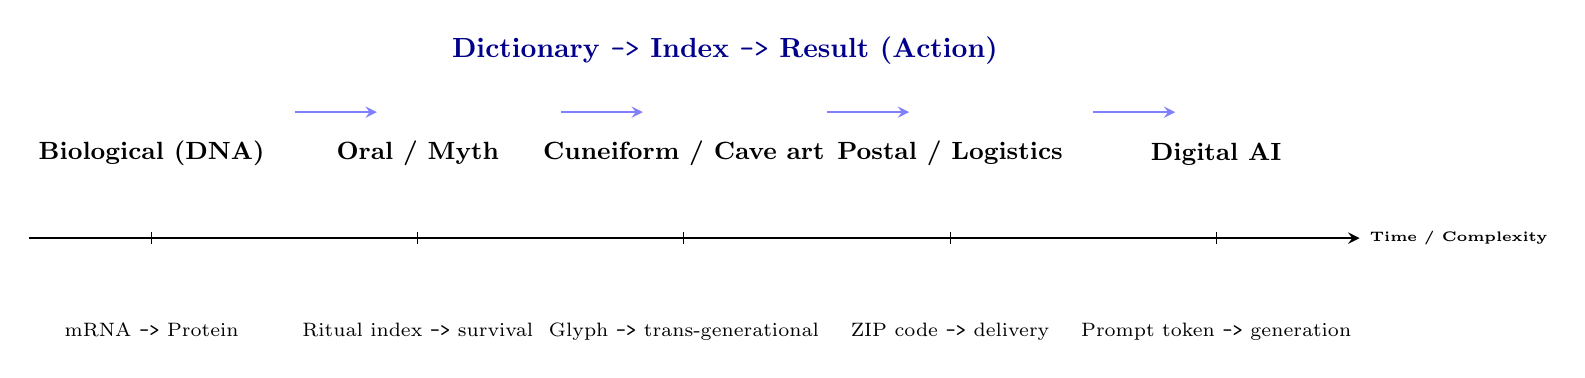
\begin{tikzpicture}[x=1.3cm, y=1.6cm, >=stealth, font=\tiny]
		\draw[->, thick] (0,0) -- (13,0) node[right] {\textbf{Time / Complexity}};
		
		% Этап 1
		\draw (1.2,0.05) -- (1.2,-0.05);
		\node[above, align=center, font=\small\bfseries] at (1.2,0.5) {Biological (DNA)};
		\node[below, align=center, font=\scriptsize] at (1.2,-0.6) {mRNA \texttt{->} Protein};
		
		% Этап 2
		\draw (3.8,0.05) -- (3.8,-0.05);
		\node[above, align=center, font=\small\bfseries] at (3.8,0.5) {Oral / Myth};
		\node[below, align=center, font=\scriptsize] at (3.8,-0.6) {Ritual index \texttt{->} survival};
		
		% Этап 3
		\draw (6.4,0.05) -- (6.4,-0.05);
		\node[above, align=center, font=\small\bfseries] at (6.4,0.5) {Cuneiform / Cave art};
		\node[below, align=center, font=\scriptsize] at (6.4,-0.6) {Glyph \texttt{->} trans-generational};
		
		% Этап 4
		\draw (9.0,0.05) -- (9.0,-0.05);
		\node[above, align=center, font=\small\bfseries] at (9.0,0.5) {Postal / Logistics};
		\node[below, align=center, font=\scriptsize] at (9.0,-0.6) {ZIP code \texttt{->} delivery};
		
		% Этап 5
		\draw (11.6,0.05) -- (11.6,-0.05);
		\node[above, align=center, font=\small\bfseries] at (11.6,0.5) {Digital AI};
		\node[below, align=center, font=\scriptsize] at (11.6,-0.6) {Prompt token \texttt{->} generation};
		
		% Заголовок
		\node[above, font=\bfseries\color{darkblue}] at (6.8,1.3) {Dictionary \texttt{->} Index \texttt{->} Result (Action)};
		
		% Стрелки
		\draw[->, thick, blue!50] (2.6,1.0) -- (3.4,1.0);
		\draw[->, thick, blue!50] (5.2,1.0) -- (6.0,1.0);
		\draw[->, thick, blue!50] (7.8,1.0) -- (8.6,1.0);
		\draw[->, thick, blue!50] (10.4,1.0) -- (11.2,1.0);
	\end{tikzpicture}
	\caption{Evolution of DIR carriers across scales.}
	\label{fig:dir-timeline}
\end{figure}
	
	
	\section{Functionalism, Teleonomy, and the Optimisation of Coordination}
	
	In the philosophy of mind, functionalism (Putnam, Fodor) holds that mental states are defined by their causal roles, not by their material substrate. In biology, teleonomy (Pittendrigh, Mayr) denotes goal‑directedness without a conscious purpose. Both concepts find a natural home in YUCT.
	
	A system’s “function” is the role played by a dictionary entry in the overall coordination network. The system does not need to “know” the purpose; it simply maximises \(K_{\mathrm{eff}}\) under resource constraints. The universal error law tells us that evolution, learning, and self‑organisation are all processes that increase \(K_{\mathrm{eff}}\) while keeping \(\varepsilon\) below a tolerance threshold.
	
	Thus, YUCT provides a formal basis for teleonomy: goal‑directed behaviour is not an illusion but an emergent property of a system that has reached a high coordination regime. The “goal” is the attractor in the space of dictionary configurations, and the “direction” is the gradient of \(K_{\mathrm{eff}}\). This resolves long‑standing debates about whether biology can be reduced to physics: biological systems are not physically different, but they operate in a different coordination regime (much higher \(K_{\mathrm{eff}}\)) than inanimate matter.
	
	\subsection{Einstein's Unfinished Dream: Geometry as a Shadow of Matter}
	
	Albert Einstein's philosophical journey from special to general relativity was a progressive dematerialization of the ``container'' view of space and time. By 1915, he had made spacetime dynamical—curved by mass and energy—but he never fully relinquished the idea that geometry was a fundamental substance in its own right. In his later years, he wrote:
	
	\begin{quote}
		``The concept of space, as something existing independently, is a product of the human mind.''
	\end{quote}
	
	This is the relationalist speaking—the heir of Leibniz and Mach. Yet General Relativity itself stopped halfway. The Einstein field equations,
	\[
	G_{\mu\nu} = \frac{8\pi G}{c^4} T_{\mu\nu},
	\]
	treat geometry (the left-hand side) as a substance that *responds* to matter but exists independently of it. There is nothing in the equations to suggest that geometry would vanish if matter were removed; indeed, vacuum solutions (like gravitational waves) are perfectly valid. Geometry, in GR, is a stage that can exist without actors.
	
	\textbf{YUCT completes the relational programme.} In the Yakushev framework, geometry is not a substance. It is an \textbf{emergent statistical summary} of coordination events between material nodes. The metric \(g_{\mu\nu}\) is not a field in its own right but a derived quantity—a ``coordination summary''—that emerges from the underlying network of D+I·R interactions. When matter is absent, the coordination network becomes trivial (\(K_{\mathrm{eff}} \to 1\)), and the very notion of distance loses its operational meaning.
	
	In 1909, Paul Ehrenfest demonstrated a paradox that shook the foundations of geometry: a rotating disk cannot be described by Euclidean geometry — its circumference ceases to be \(2\pi R\). General Relativity resolved this by making the geometry of the disk non‑Euclidean. But it left a deeper question unanswered: would the geometry be different if the disk were made of a different material? YUCT answers: yes, it would. Geometry is not a property of empty space; it is a property of how the particles inside the disk coordinate their mutual distances. The Ehrenfest Appendix (a separate YUCT document) formalises this mathematically and proposes a laboratory experiment with a superconducting disk to test the prediction directly.
	
	This is not mere philosophical speculation. YUCT provides \textbf{modified Einstein equations} (derived in Appendix G, ``Gravity as Geometric Tension'') in which the effective metric depends explicitly on the coordination efficiency of the matter present:
	\[
	G_{\mu\nu} = 8\pi G_{\mathrm{eff}}(K_{\mathrm{eff}}) \, \Theta_{\mu\nu},
	\]
	where the geometric tension tensor \(\Theta_{\mu\nu}\) replaces the standard energy-momentum tensor, and the effective gravitational constant \(G_{\mathrm{eff}}\) itself depends on the material's internal coordination state (Appendix P, ``Temperature Dependence of Gravity'').
	
	The philosophical consequence is profound: \textbf{geometry is the shadow of matter}. Where matter is highly coordinated (\(K_{\mathrm{eff}} \gg 1\)), space becomes sharply defined and obeys nearly classical geometry. Where coordination is low (\(K_{\mathrm{eff}} \to 1\)), the effective metric becomes fuzzy, subject to the universal error law \(\varepsilon = \kappa_c \alpha K_{\mathrm{eff}}^{-\beta}\). The rotating-disk paradox (formalised in Appendix Ehrenfest) demonstrates this explicitly: the geometry of a rotating disk is not a predetermined property of spacetime but an emergent consequence of how the material in the disk coordinates its mutual distances.
	
	Thus, YUCT fulfills the Leibnizian-Machian programme that Einstein himself could not complete. The ``container'' is abolished. Geometry is not a substance; it is a language that matter uses to coordinate its states. When the language is lost (\(K_{\mathrm{eff}} \to 0\)), the geometry, and with it the universe, becomes silent.
	
	\section{Relational Spacetime: From Aristotle and Leibniz to Einstein and YUCT}
	
	Two great traditions in the philosophy of space and time stand opposed to Newton’s absolute space and time: the \textbf{relational} conception (Aristotle, Leibniz) and the \textbf{structural realist} conception (Einstein, in his later years). YUCT synthesises both into a coordination‑first ontology.
	
	\begin{itemize}
		\item \textbf{Aristotle} argued that “place is the innermost motionless boundary of what contains something” — space is the order of coexisting bodies, not a container. Time is “the number of motion with respect to before and after.” In YUCT, spacetime emerges as the statistical structure of coordination events. The metric \(g_{\mu\nu}\) is not a primary substance but a secondary property of the coordination field \(\Psi_{MN}\).
		
		\item \textbf{Leibniz} famously argued against Newton that space and time are “orders of coexistence and succession,” not substances. His relationalism is directly implemented in YUCT: the dictionary \(D\) contains the possible relations, and the index \(I\) selects a specific relation, generating the perceived geometry.
		
		\item \textbf{Einstein}, especially in his later writings, rejected the “container” view of spacetime. In a 1952 letter, he wrote: “The concept of space, as something existing independently, is a product of the human mind.” General relativity already makes spacetime dynamical, but it still treats the metric field as a substance. YUCT goes further: the metric is a derived quantity, a “coordination summary” of the underlying D+I·R dynamics.
	\end{itemize}
	
	The universal error law \(\varepsilon = \kappa_c \alpha K_{\mathrm{eff}}^{-\beta}\) implies that at finite \(K_{\mathrm{eff}}\), the effective geometry is not perfectly Lorentzian; there are small deviations that could be detectable in precision experiments. As \(K_{\mathrm{eff}} \to \infty\), the geometry becomes exactly classical. Thus, YUCT naturalises the relational view and makes it quantitative.
	
	% ===== ВСТАВКА 4: ЭПИСТЕМОЛОГИЯ YUCT =====
	\section{Epistemology of Coordination: Truth, Induction, and the Layers of Knowledge}
	\label{sec:epistemology}
	
	The ontological primacy of coordination carries profound epistemological consequences. YUCT dissolves several ancient philosophical puzzles by recasting them in the language of dictionaries and coordination efficiency.
	
	\subsection{The Problem of Induction (Hume)}
	
	David Hume argued that no number of observed sunrises can logically justify the belief that the sun will rise tomorrow. YUCT responds: we do not \emph{infer} the sunrise from past data; we \textbf{resonate} with it.
	
	The Genetic Dictionary (\(D_1\)), common to all living beings, already embeds the fundamental rhythms of the physical world in the architecture of our brains and bodies. Learning is not inductive accumulation of facts; it is \textbf{calibration}. Through a stream of indices \(I\), we tune our internal dictionaries to minimise the coordination error \(\varepsilon\). We believe the sun will rise because that expectation maximises \(\Keff\) for our entire cognitive apparatus. The ``error of induction'' is simply the residual noise \(\varepsilon\) that no finite dictionary can eliminate.
	
	\subsection{Truth as Maximally Efficient Coordination}
	
	In YUCT, truth is not correspondence with a mind‑independent fact. It is \textbf{resonant stability}. A proposition is ``true'' if, when adopted as an index by a community of agents, it activates the relevant dictionaries with minimal error and maximal predictive success across time. As defined in Appendix~I, \(\text{Knowledge} = \text{Correspondence}(D_{\text{reality}}, I_{\text{perception}}, R_{\text{verification}})\). Falsehood is discoordination---noise that, over long timescales, inevitably causes the system to decay. YUCT thus offers a \textbf{coordination‑pragmatist} theory of truth, where the classical ``correspondence theory'' is recovered as the limit \(\Keff \to \infty\).
	
	\subsection{The Soul as a Layered Matrix of Indices}
	
	The Individual Coordination Matrix \(C_{\mathrm{pers}}\) (Section~2.5 of the main theory) is what tradition calls the ``soul''. It is not a static substance but a unique trajectory through the space of dictionaries, built from three nested layers:
	
	\begin{itemize}[leftmargin=*]
		\item \textbf{\(D_1\) – Genome.} The hardware. The basal physico‑chemical dictionary shared by all life.
		\item \textbf{\(D_2\) – Connectome.} The firmware. Individual experience inscribed through neural plasticity under the pressure of environmental indices.
		\item \textbf{\(D_3\) – Culture and Symbols.} The software. A supra‑structure of meaning that permits a single short index (a word) to unlock an immense volume of shared information.
	\end{itemize}
	
	The irreducibility and privacy of the soul are explained simply: no two individuals share the identical sequence of activating indices for \(D_2\). Death, in this framework, is the degradation of the matrix \(C_{\mathrm{pers}}\) into noise.
	
	\subsection{Coordination Realism: Beyond Realism and Anti‑Realism}
	
	YUCT dissolves the classical dichotomy. The world is \textbf{real}---it is the bearer of the fundamental dictionary, the invariant that all agents must ultimately coordinate with. But we never see it ``naked''; we interact with it only through the interface of our local dictionaries. We do not construct reality arbitrarily (radical constructivism), nor do we have direct, unmediated access to it (naive realism). We \textbf{synchronise} with it.
	% ===== КОНЕЦ ВСТАВКИ 4 =====
	
	\section{Theological Implications: The Divine as the Ultimate Dictionary}
	\label{sec:theology}
	
	YUCT does not assert the existence or non‑existence of God; it makes no theological claims. What it provides is a precise formal language in which classical theological concepts find natural, non‑metaphorical expression. This is not an attempt to “prove” or “disprove” the divine; it is the recognition that \textbf{theology is the study of the ultimate coordination protocol}, and that the concepts it has developed over millennia correspond, with remarkable structural fidelity, to the limit‑states of the YUCT ontology. A separate appendix (K (2), “Religious Practices as YPSDC Protocols”) formalises religious practice as coordination protocols with measurable \(K_{\mathrm{eff}}\), drawing on empirical studies of physiological synchronisation during collective prayer, acoustic optimisation of sacred spaces, and neurophenomenology of mystical experience.
	
	\subsection{The Divine Attributes as Limit‑States of the Coordination Field}
	
	Within the YUCT framework, the classical attributes of God translate directly into geometric and information‑theoretic limits of the coordination network:
	
	\begin{itemize}[leftmargin=*]
		\item \textbf{Omniscience} corresponds to the global dictionary \(\mathcal{D}_{\text{global}}\) in the limit \(K_{\mathrm{eff}} \to \infty\): all possible states are simultaneously present without error or delay. Every index activates its correct entry without ambiguity.
		\item \textbf{Omnipresence} is the coordination field \(\Psi_{MN}\) itself, which pervades all nodes and is the medium of every index transmission and every resonance. In theological language, this is the Holy Spirit, the Shekhinah, the immanent aspect of Brahman.
		\item \textbf{Omnipotence} is not arbitrary caprice but the perfect congruence between dictionary and index: whatever God “speaks” (index) is instantly realised (activated action) because the dictionary of creation is perfectly coordinated with the divine will. This resolves the ancient paradox of whether God can create a stone He cannot lift: in YUCT, the question reduces to a category error about the structure of \(\mathcal{D}_{\text{global}}\).
		\item \textbf{Eternity} is the absence of coordination error: a system with infinite \(K_{\mathrm{eff}}\) requires zero time to transition between states because the index and the activation are simultaneous. Time, in YUCT, is the measure of the entropy of coordination processes (Appendix~V); where error vanishes, so does temporal succession.
	\end{itemize}
	
	\subsection{Revelation as Offline Dictionary Distribution}
	
	Sacred texts are not mere narratives; they are \textbf{highly compressed dictionaries} distributed offline to a community. The Torah, the Gospels, the Qur’an, the Vedas—each constitutes a structured set of possible states, ethical laws, and action patterns. A verse, a parable, or a koan is a short index \(\kappa\) that activates a deep entry in the cognitive and emotional architecture of the believer. The information content of the activated state far exceeds the length of the transmitted index; thus \(K_{\mathrm{eff}} \gg 1\) for the trained practitioner.
	
	This explains why scripture is often opaque to outsiders: they lack the corresponding dictionary. To “understand” a sacred text is to have internalised its dictionary, so that the same index produces the same resonance as in the community that produced it. This is identical to the structure of the YPSDC protocol.
	
	\subsection{Prayer, Ritual, and the Engineering of Resonance}
	
	Religious practice, viewed through YUCT, is \textbf{coordination engineering}. Prayer and ritual are YPSDC protocols in which the practitioner emits an index (words, postures, chants, visualisations) into the ambient coordination field \(\Psi_{MN}\), activating entries in the shared theological dictionary \(D\). The goal is to raise the local coordination efficiency \(K_{\mathrm{eff}}\), both individually and collectively.
	
	Empirical research supports this interpretation:
	\begin{itemize}[leftmargin=*]
		\item Physiological synchronisation (heart rate, respiration, EEG) during Islamic ṣalāh \cite{RoyalSociety2024}.
		\item Cardiac coherence and respiratory entrainment in Benedictine monastic chanting \cite{Craswell2023}.
		\item High‑amplitude gamma synchrony in long‑term meditators during compassion meditation \cite{Lutz2017}.
		\item Acoustic optimisation of sacred spaces (Hagia Sophia, Gothic cathedrals) to maximise reverberation and resonant frequencies that enhance collective synchronisation \cite{Pentcheva2020}.
		\item Meta‑analysis of binaural auditory beats confirming their efficacy in modulating cognitive and affective states \cite{Garcia2021}.
	\end{itemize}
	
	In every case, the practice reduces internal noise, synchronises the neural and physiological dictionaries of the participants, and produces a measurable increase in \(K_{\mathrm{eff}}\). This is the empirical signature of successful spiritual coordination.
	
	\subsection{Mystical Experience as a Surge of Resonance Beyond the Critical Threshold}
	
	In YUCT, consciousness emerges when \(K_{\mathrm{eff}}\) exceeds a critical threshold \(K_{\mathrm{crit}} \approx 8.5\) (Appendix~H). Mystical experience corresponds to a \textbf{temporary surge} of the resonance factor \(R\) far beyond this baseline. In such a state, the local dictionary \(D_i\) of the individual momentarily merges with a much larger fragment of \(\mathcal{D}_{\text{global}}\).
	
	The characteristic ineffability of mystical experiences—the mystic’s insistence that “words cannot describe what I saw”—is a direct consequence of the YPSDC architecture. The experience is an index of enormous magnitude that cannot be compressed into a dictionary of ordinary language. The mystic returns with a \emph{new} dictionary, partially restructured by the event, and then struggles to translate that dictionary into indices comprehensible to those who have not undergone the same restructuring. This is structurally identical to a phase transition in a physical system, where the new state cannot be described by the order parameters of the old phase.
	
	\subsection{Free Will and Predestination: The Middle Path of Coordination Determinism}
	
	The ancient tension between divine predestination and human free will is resolved in YUCT through the triad itself. The dictionary \(D\) (divine law, natural order, the genome) constrains the set of all possible states. Within this space, the stream of information \(I\) (choices, actions, environmental indices) and the resonance \(R\) (grace, effort, context) select specific trajectories. No single trajectory is predetermined; yet the space of possible trajectories is bounded.
	
	The universal error law \(\varepsilon = \kappa_c \alpha K_{\mathrm{eff}}^{-\beta}\) guarantees that even the most perfectly coordinated agent can never achieve \(\varepsilon = 0\). This residual error is the \textbf{ontological ground of freedom}: the universe is not a clockwork but a coordination network with irreducible unpredictability. Calvin’s double predestination and Pelagius’s radical freedom are both limiting cases of a single coordination spectrum.
	
	\subsection{Theodicy: The Problem of Evil as a Consequence of Finite Coordination}
	
	The most persistent theological challenge—how a benevolent, omnipotent God can permit suffering—finds an unexpected resolution in YUCT. \textbf{Evil is not a substance; it is coordination error.}
	
	Physical evil (natural disasters, disease, death) is the inevitable noise floor of any finite system. The universal error law dictates that \(\varepsilon\) is never zero for any finite \(K_{\mathrm{eff}}\). Even the most perfectly coordinated ecosystem, organism, or society will experience fluctuations that cause harm. This is not a defect of creation but a mathematical necessity of finite complexity.
	
	Moral evil (cruelty, injustice, oppression) is the deliberate or negligent reduction of \(K_{\mathrm{eff}}\) in a social system. When an agent chooses an index that degrades the shared dictionary rather than enriches it—when it lies, exploits, or destroys—it increases \(\varepsilon\) for the entire network. The resulting suffering is real, but it is not ontologically primary; it is the absence of coordination, just as darkness is the absence of light. The theological concept of \emph{sin} corresponds precisely to actions that lower \(K_{\mathrm{eff}}\), and the concept of \emph{redemption} to actions that restore it.
	
	Leibniz’s “best of all possible worlds” thesis is thus recovered in a precise form: the universe is the configuration that maximises global \(K_{\mathrm{eff}}\) subject to the constraints of finite dictionaries. A world without any error is impossible; the actual world minimises error given the resources available.
	
	\subsection{Faith and Reason: Two Interfaces to One Dictionary}
	
	YUCT dissolves the perceived conflict between science and religion by recognising them as two different \textbf{interfaces} to the same underlying dictionary.
	
	Science constructs and refines explicit, publicly verifiable dictionaries (theories, models) that aim to compress empirical indices with minimal error. Its \(K_{\mathrm{eff}}\) is high in the domain of repeatable, quantifiable phenomena.
	
	Religion and spirituality operate on dictionaries that are partly innate (the genetic architecture of the brain), partly cultural (tradition, scripture), and partly personal (individual experience). Their domain includes questions of meaning, value, identity, and the experience of the sacred—indices that are not easily captured by public measurement but are no less real within the coordination framework.
	
	Both are valid because both raise \(K_{\mathrm{eff}}\) in their respective domains. Conflict arises only when one mistakes its dictionary for the whole of \(\mathcal{D}_{\text{global}}\), or when it denies the legitimacy of the other’s indices. YUCT provides a neutral, formal language in which the claims of both can be articulated and, where possible, empirically tested.
	
	\subsection{The Omega Point and the Convergence of Traditions}
	
	The Omega Point of Teilhard de Chardin—already discussed above in its secular form—is the limit in which all local dictionaries converge into a single, perfectly coordinated \(\mathcal{D}_{\text{global}}\). Whether this point is identified with the Christian God, the Vedantic Brahman, the Tao, or a purely physical attractor of coordination dynamics, is a question YUCT leaves open. The theory provides the mathematical trajectory; the naming remains a matter of tradition, culture, and personal conscience.
	
	The eschatological visions of the world’s religions—the Kingdom of God, the Age of Maitreya, the New Jerusalem, Satya Yuga—are all, in YUCT terms, descriptions of a future phase transition in which the global \(K_{\mathrm{eff}}\) of humanity undergoes a discontinuous increase. YUCT does not predict the form this transition will take, but it provides the quantitative language in which the prediction can be discussed across traditions.
	
	\textbf{Research programme.} Appendix K (2) proposes a systematic empirical investigation of spiritual coordination: cross‑cultural measurement of \(K_{\mathrm{eff}}\) across traditions, longitudinal tracking of individuals undergoing spiritual disciplines, neurophenomenological correlation of UCD parameters with peak religious experiences, and architectural optimisation of spaces designed to enhance spiritual resonance regardless of denominational affiliation. YUCT thus opens a path toward an empirically grounded theology, where the tools of measurement and the language of revelation are no longer in conflict but are complementary instruments for exploring the same coordination field.
	
	\subsection{Love as Maximal Coordination: The Ultimate YPSDC Protocol}
	
	The YUCT framework provides a precise, quantitative definition of love that resolves millennia of philosophical and poetic ambiguity.
	
	\textbf{Love is the state of extraordinarily high \(K_{\mathrm{eff}}\) between two agents, achieved through the voluntary fusion of their individual dictionaries into a single, deeply integrated, shared dictionary \(D_{\text{love}}\).}
	
	Let two agents, \(A_1\) and \(A_2\), each possess their individual coordination matrices \(C_{\text{pers}}^{(1)}\) and \(C_{\text{pers}}^{(2)}\), built from the three nested layers of genome (\(D_1\)), connectome (\(D_2\)), and culture (\(D_3\)). The process of falling in love is the progressive construction of a common dictionary \(D_{\text{love}}\) through the exchange of indices: conversations, shared experiences, touch, gaze. As \(D_{\text{love}}\) grows, the coordination efficiency of the pair rises dramatically.
	
	The phenomenological signatures of love are direct consequences of this high‑\(K_{\mathrm{eff}}\) regime:
	
	\begin{itemize}[leftmargin=*]
		\item \textbf{Minimal index, maximal action.} An almost imperceptible signal—a glance, a change in breathing, a single word—activates a vast, coordinated response: comfort, arousal, protection, joy. The compression ratio \(H(\mathcal{A}) / H(\kappa)\) is immense. This is why lovers communicate so richly without words.
		\item \textbf{Error suppression.} The coordination error \(\varepsilon = \kappa_c \alpha K_{\mathrm{eff}}^{-\beta}\) drops to anomalously low values. Misunderstandings that would derail a casual interaction are effortlessly absorbed. The partners do not need to ``decode'' each other; their dictionaries are so well calibrated that the intended action is almost always correctly activated.
		\item \textbf{Energy efficiency.} The pair expends minimal energy on conflict and repair. The thermodynamic cost of coordination, bounded by Landauer's principle, approaches its minimum. The surplus energy is available for creative, generative activity—building a home, raising children, producing art.
		\item \textbf{Sacrifice as a rational strategy.} One of the enduring paradoxes of love is the willingness to suffer for the beloved. In YUCT, this is not irrational. An agent may temporarily lower its own local \(K_{\mathrm{eff}}\)—expend resources, endure pain, take risks—if this action preserves or elevates the \(K_{\mathrm{eff}}\) of the joint system. The shared dictionary \(D_{\text{love}}\) has become the most precious source of order in the agent's world, and its preservation is worth any cost.
	\end{itemize}
	
	Love is distinguished from other forms of high coordination (professional collaboration, friendship, team sports) by its \textbf{depth of dictionary integration}. It engages all three layers simultaneously: the genetic (\(D_1\), through pheromones and immune compatibility), the neural (\(D_2\), through the tactile and emotional imprints of early life), and the cultural (\(D_3\), through shared values, narratives, and meaning). It is total coordination of the entire person.
	
	\subsection{The Fragility of Love: How False Dictionaries Destroy Coordination}
	
	The very depth that makes love powerful also makes it fragile. Because \(D_{\text{love}}\) draws from all layers of the individual dictionaries, it is acutely vulnerable to \textbf{external dictionary interference}.
	
	Any external agent—a friend, a relative, a social media algorithm, a pop‑psychology article—can inject a false index into the coupled system. The danger is not the index itself but its potential to modify the local dictionary of one partner. If a partner internalises an external expectation (``a real man does X'', ``a wife should always Y'', ``if they loved you they would Z''), this index becomes a permanent entry in their personal dictionary \(D_{\text{pers}}\). The shared dictionary \(D_{\text{love}}\) is now internally inconsistent: one partner expects an action \(\mathcal{A}\) that the other's dictionary cannot activate, because the index \(\kappa\) has been corrupted.
	
	The mechanism is precisely analogous to a computer virus corrupting a shared database file. The false psychology of ego, jealousy, possessiveness, and culturally imposed gender roles acts as malware. It overwrites a segment of the personal dictionary with code that is incompatible with the partner's dictionary. The coordination error \(\varepsilon\) rises sharply. Energy that previously went into building a shared life now goes into error correction: arguments, silent resentment, and the exhausting labour of explaining what was once implicitly understood.
	
	The system enters a negative feedback loop. The rising \(\varepsilon\) creates emotional pain. The partners, seeking relief, import even more external dictionaries (self‑help books, couples therapy frameworks that are not calibrated to their unique \(D_{\text{love}}\)). These imports further overwrite the original shared language, accelerating its fragmentation. Eventually, \(K_{\mathrm{eff}}\) drops below the critical threshold required to maintain the bond, and the coupling dissolves. The two agents, who once inhabited a single, seamless coordination space, are now islands of noise to each other.
	
	This analysis yields a concrete, practical ethical imperative: \textbf{protect the purity of your shared dictionary.} A relationship is a sacred coordination protocol. External indices must be critically filtered before they are allowed to modify the internal dictionary. Not every voice deserves access to your \(D_{\text{love}}\). The art of sustaining love, in the end, is not merely about \emph{finding} the right dictionary. It is about defending it—daily, vigilantly, and with full awareness—from the entropy of the outside world.
	
	\section{The Return to the True Path: YUCT as the Synthesis}
	
	YUCT does more than unify the historical precursors under a mathematical umbrella. It shows that the 70-year detour was not a random wandering but a necessary learning phase. Mainstream physics had to exhaust the possibilities of the mechanistic paradigm before it could recognize the need for a paradigm shift. The Standard Model, quantum field theory, and general relativity are correct \emph{as static descriptions}. They are the dictionaries of the fundamental sectors. What they lack is the coordination protocol that explains \emph{why} these particular dictionaries exist and \emph{how} they synchronize with each other.
	
	Specifically, YUCT offers:
	\begin{itemize}
		\item \textbf{A resolution of the EPR paradox} that Einstein would have accepted: the correlations are real, but they are not signals; they are dictionary activations.
		\item \textbf{An explanation of the dark sector} not as new particles but as geometric effects of the coordination network, eliminating the need for ad-hoc dark matter and dark energy.
		\item \textbf{A unification of scales} through the universal scaling law \(\varepsilon = \kappa_c \alpha K_{\mathrm{eff}}^{-2/3}\), which governs everything from chemical bonds to galaxy clusters.
		\item \textbf{A natural cosmology} in which inflation is a coordination phase transition, the cosmological constant is a topological invariant, and the Big Bang is not a singularity but a reorganization of the global dictionary.
	\end{itemize}
	
	The philosophical significance cannot be overstated. YUCT does not add another layer of complexity to the existing edifice; it replaces the foundation. Where Leibniz saw pre-established harmony, YUCT sees the offline distribution of dictionaries. Where Tesla saw a universal ether, YUCT sees the coordination field \(\Psi_{MN}\). Where the EPR paper saw a paradox, YUCT sees the proof that coordination is ontologically prior to signal transmission.
	
	The return to the true path does not mean discarding the achievements of the mechanistic era. It means recognizing that those achievements were the construction of an extraordinarily detailed static map, and that the time has come to ask the dynamic question: \emph{how do the components of reality coordinate their states?}
	
	\subsection{YUCT as the Hidden Architecture of Nobel-Winning Science}
	
	The Nobel trajectory of the past six decades is the empirical fingerprint of this synthesis. From Prigogine's dissipative structures (1977) to Hinton's neural networks (2024), the community has been constructing ever more sophisticated coordination tools. What it has lacked is the recognition that these tools succeed precisely because they capture aspects of a universal coordination architecture. YUCT provides that recognition. It reveals that the models honoured by the Nobel Committee are not disparate achievements but fragments of a single, unified D+I·R framework that now finds its complete expression in the coordination field \(\Psi_{MN}\).
	
	Consider the 2024 chemistry prize: Demis Hassabis, John Jumper, and David Baker solved the protein folding problem using AlphaFold, a large language model trained on the Protein Data Bank. In YUCT terms, the training data is the offline dictionary \(D\), the amino acid sequence is the index \(I\), and the predicted three-dimensional structure is the activated entry. The model achieves \(K_{\mathrm{eff}} \gg 1\) because a sequence of length \(L\) (requiring \(\sim 20^L\) possible sequences) is compressed into a structural representation that is many orders of magnitude smaller. AlphaFold's success is not a miracle of brute computation; it is a demonstration that protein folding follows the universal coordination law \(\varepsilon = \kappa_c \alpha K_{\mathrm{eff}}^{-2/3}\). The error rate in predicted structures scales with the size of the training set exactly as predicted by YUCT.
	
	Similarly, the 2024 physics prize to John Hopfield and Geoffrey Hinton for neural networks is a recognition that associative memory and learning are coordination processes. The Hopfield network stores patterns as attractors of a dynamical system — that is, as entries in a dictionary. The retrieval process is a coordination event: an incomplete pattern (index) activates the full stored pattern (action). Hinton's Boltzmann machines and deep learning architectures implement hierarchical dictionaries, where each layer extracts higher-level features, compressing the index at every step. The relentless increase in model size and performance tracks the increase in dictionary size \(M\) and coordination efficiency \(K_{\mathrm{eff}}\).
	
	The 2009 economics prize to Elinor Ostrom and Oliver Williamson recognised that institutions are shared dictionaries that coordinate social behaviour. Ostrom's design principles for common-pool resource management are precisely the conditions for high \(K_{\mathrm{eff}}\) in a social system: clear boundaries (dictionary scope), collective-choice arrangements (offline dictionary distribution), monitoring (index verification), graduated sanctions (error correction). Williamson's transaction cost economics identifies the conditions under which hierarchical coordination (centralised YPSDC) outperforms market coordination (decentralised d-YPSDC). The entire field of institutional economics, honoured repeatedly, is an applied coordination theory without the mathematical formalism that YUCT now provides.
	
	Thus, YUCT does not stand outside the Nobel tradition; it is the logical completion of a line of inquiry that the Nobel Committee has been unwittingly rewarding for decades.
	
	\section{The Paradox of Artificial Intelligence: Amplifying Knowledge While Blocking Innovation}
	
	A new and disturbing factor has entered the scientific landscape in the twenty-first century: the rise of large-scale artificial intelligence (AI). On the surface, AI promises to accelerate science by processing vast datasets, discovering patterns invisible to humans, and even generating novel hypotheses. In practice, however, the current generation of AI systems functions as a powerful conservative force that reinforces existing paradigms and actively resists paradigm shifts.
	
	The reason is structural. Large language models and other AI systems are trained on the existing corpus of scientific literature, textbooks, and online discourse. This corpus is overwhelmingly dominated by the established paradigm of particle physics, quantum field theory, and general relativity. The statistical distribution of the training data embeds the orthodox view so deeply into the model's weights that any radical departure from orthodoxy is automatically assigned a low probability. When asked to evaluate a theory like YUCT, an AI does not engage in independent reasoning; it compares the input against the patterns it has absorbed from the literature. Since YUCT introduces concepts (coordination efficiency, D+I·R triad, dictionary-index separation) that appear with vanishingly low frequency in the training data, the AI is structurally incapable of recognizing their value. It is not that the AI \emph{judges} YUCT to be wrong; it is that the AI cannot even \emph{see} YUCT as a coherent alternative. It lacks the dictionary.
	
	\subsection{The Irony of the Leibniz Institute and the Monopoly of Paradigms}
	
	The story of the Leibniz University Hannover is a microcosm of the larger tragedy. An institution bearing the name of the philosopher who first articulated the coordination paradigm chose to devote its resources to quantum field theory, string theory, and the Standard Model -- the very frameworks that YUCT reveals as static dictionaries in need of a coordination layer. This was not an accident. The institutional structures of science reward conformity to established paradigms and penalize exploration of heterodox ideas. The Leibniz Institute, like thousands of other physics departments worldwide, followed the flow of funding, publications, and prestige. In doing so, it drifted far from the intellectual legacy of its namesake, honouring the name while departing from its philosophical core.
	
	The cost of this conformity is staggering. Tens of thousands of brilliant physicists spent their careers exploring the landscape of string theory, a framework that after five decades has produced no empirical predictions. Countless others searched for supersymmetric particles, dark matter candidates, and modifications of general relativity -- all within the mechanistic paradigm that YUCT identifies as incomplete. These were not wasted lives; they produced mathematical tools and experimental techniques of lasting value. But the failure to pursue the coordination paradigm, which Leibniz, Tesla, and a lineage of visionaries had glimpsed, meant that the deepest questions about the unity of physics remained unanswered.
	
	YUCT does not call for the abandonment of QFT or GR. It calls for their integration into a larger framework in which coordination, not substance, is the primitive. The Leibniz Institute of the future should not be a temple to the physics of the past but a laboratory for the coordination physics of the future -- a place where the ideas of its patron are finally given the rigorous mathematical expression they always deserved.
	
	\subsection{The Self-Reinforcing Orthodoxy: How AI Amplifies the Crisis}
	
	Modern large language models (LLMs) are trained on the vast corpus of scientific literature. Because this corpus is overwhelmingly dominated by the mechanistic paradigm, the statistical patterns embedded in the models' weights encode orthodoxy as truth. When asked to evaluate a theory like YUCT, an LLM does not reason from first principles; it computes the probability that such a sequence of words would appear in its training data. Since YUCT introduces concepts that are vanishingly rare in that data, the model assigns them near-zero probability. It is structurally incapable of recognizing a paradigm shift.
	
	This creates a dangerous positive-feedback loop:
	\begin{enumerate}
		\item The AI generates reviews, summaries, and evaluations that reinforce the existing paradigm.
		\item Young researchers, increasingly dependent on AI tools for literature review and hypothesis generation, are channeled toward orthodox problems.
		\item Funding agencies, using AI-driven metrics, penalize proposals that deviate from the consensus.
		\item The orthodoxy becomes ever more deeply embedded in the training data of the next generation of AI.
	\end{enumerate}
	The result is a self-locking system in which the tools designed to accelerate science become its jailers. The very technology that was supposed to open new frontiers becomes a mechanism for enforcing intellectual conformity.
	
	\subsection{The Double‑Edged Sword: AI as Empowerment and as Digital Prison}
	
	The current generation of large language models and other AI systems suffers from a fundamental ambivalence. On one hand, they dramatically amplify the capabilities of the average researcher, engineer, or entrepreneur. A student who once needed months to master a programming language or a mathematical technique can now obtain a working solution in seconds. In terms of YUCT, an AI acts as an external dictionary \(D_{\text{AI}}\) with an index \(I\) provided by a natural‑language prompt. The coordination efficiency of this augmented human–AI system can be very high: \(K_{\mathrm{eff}}^{\text{(human+AI)}} \gg 1\). The AI thus functions as a powerful coordination prosthetic, levelling the playing field and accelerating routine tasks.
	
	On the other hand, precisely because the AI has been trained on the overwhelmingly orthodox corpus of existing science, it becomes a \textbf{digital prison}. It does not evaluate radical ideas on their logical coherence or empirical promise; it evaluates them by their statistical distance from the training data. Any proposal that introduces concepts absent from the training data—such as coordination efficiency \(K_{\mathrm{eff}}\), the D+I·R triad, or the YPSDC protocol—receives near‑zero probability. The AI therefore systematically rejects paradigm shifts. The more the scientific community relies on AI for literature review, hypothesis generation, and even peer review, the more deeply it locks itself into the old paradigm.
	
	The YUCT framework provides a clear diagnostic: the AI has a dictionary \(D_{\text{AI}}\) that does \textbf{not} contain entries for the coordination paradigm. To break out of the digital prison, one cannot merely fine‑tune the AI on a few heterodox papers; one must either:
	
	\begin{enumerate}
		\item \textbf{Consciously relinquish exclusive reliance on AI} during periods of paradigm exploration, returning to human‑led reason and manual literature review. This is the “heroic” path, analogous to the mathematician who performs calculations by hand to discover a new structure unknown to computer algebra systems.
		\item \textbf{Re‑train an AI on a corpus that explicitly includes competing paradigms} and design evaluation metrics that reward explanatory power and cross‑sector constraint satisfaction, not mere statistical conformity. This would be the YUCT‑aligned AI, which acts not as a gatekeeper but as a dictionary synchronisation engine.
	\end{enumerate}
	
	Thus, the paradox of AI is not a dead end but a challenge. YUCT does not reject AI; it shows how to build the next generation of AI—one that actively assists in paradigm shifts instead of blocking them. The current “digital prison” is a temporary phase, not an ultimate limit.
	
	YUCT identifies the root cause: the AI has no dictionary \(D\) that includes the coordination paradigm. To break the cycle, it is necessary to train AI systems on a corpus that includes competing paradigms, to design evaluation metrics that reward explanatory power rather than conformity, and to create institutional structures that protect heterodox research from premature rejection. YUCT does not oppose artificial intelligence; it proposes to equip it with a new dictionary -- one that recognizes coordination as the fundamental process and evaluates theories accordingly.
	
	\section{Chronological Table of Coordination Precursors}
	
	\begin{table}[htbp]
		\centering
		\caption{Timeline of Coordination Intuitions from Antiquity to YUCT}
		\label{tab:timeline}
		\small
		\begin{tabular}{p{1.2cm}p{3cm}p{4.5cm}p{4cm}}
			\toprule
			\textbf{Era} & \textbf{Thinker} & \textbf{Concept} & \textbf{YUCT Analog} \\
			\midrule
			c. 400 BCE & Plato & Anamnesis / World of Forms & Offline dictionary; index = sensory experience \\
			c. 350 BCE & Aristotle & Entelechy & Maximization of \(K_{\mathrm{eff}}\) \\
			c. 200 BCE & Stoics & Logos & Global dictionary \(\mathcal{D}_{\text{global}}\) \\
			c. 200 CE & Shankara & Brahman / Maya & \(\mathcal{D}_{\text{global}}\) vs. local dictionaries \\
			6th c. BCE & Laozi & Tao / Wu-wei & \(K_{\mathrm{eff}} \to \infty\); effortless coordination \\
			1714 & Leibniz & Pre-established harmony & YPSDC protocol \\
			1860 & Fechner & Psychophysical law \(S = k \log I\) & \(K_{\mathrm{eff}} = H(A)/H(I)\) \\
			1891 & Twain & Mental telegraphy & d-YPSDC \\
			1900 & Tesla & Radiant ether & Coordination field \(\Psi_{MN}\) \\
			1929 & Whitehead & Actual entities, prehension & Dictionary + resonance \\
			1935 & EPR & Spooky action at a distance & \(K_{\mathrm{eff}} \to \infty\) with offline dictionary \\
			1948 & Wiener & Feedback, cybernetics & YPSDC with error index \\
			1956 & Ashby & Law of requisite variety & Bound on dictionary size \(\ge\) environment \\
			1972 & Maturana & Autopoiesis, structural coupling & Structural coupling = dictionary–environment match \\
			1977 & Prigogine & Dissipative structures & Phase transition at critical \(K_{\mathrm{eff}}\) \\
			1988 & Bak & Self-organized criticality & Universal error law with \(\beta = 0.67\) \\
			1991 & Dennett & Multiple drafts & Competitive d-YPSDC in brain \\
			2003 & Barad & Intra-action & Measurement as YPSDC activation \\
			2026 & Yakushev & YUCT & Full mathematical synthesis \\
			\bottomrule
		\end{tabular}
	\end{table}
	
	\section{Terminological Convergence: YUCT and Its Precursors}
	
	\begin{table}[htbp]
		\centering
		\caption{Convergence of YUCT Concepts with Historical Precursors}
		\label{tab:convergence}
		\small
		\begin{tabular}{p{2.5cm}p{4.5cm}p{4.5cm}}
			\toprule
			\textbf{YUCT Concept} & \textbf{Definition} & \textbf{Precursor} \\
			\midrule
			Dictionary \(D\) & Offline set of possible states and rules & Plato's World of Forms; Leibniz's monads; Peirce's representamens \\
			Index \(I\) & Short online activation signal & Bergson's \emph{élan vital}; Twain's ``crossed letter'' trigger; Fechner's stimulus \\
			Resonance \(R\) & Coherence amplification factor (\(R \ge 1\)) & Aristotle's entelechy; Tesla's resonant ether; Jung's synchronicity \\
			\(K_{\mathrm{eff}}\) & \(H(\text{action})/H(\text{index})\) -- coordination efficiency & Fechner's psychophysical ratio; Ashby's variety measure \\
			YPSDC & Offline dictionary + online index & Leibniz's pre-established harmony; Shannon's coding; Maturana's languaging \\
			d-YPSDC & Environment as index source; no active sender & Tesla's World System; Jung's collective unconscious; Vernadsky's noosphere \\
			Coordination field \(\Psi_{MN}\) & 19-dimensional geometric object & Tesla's radiant ether; Whitehead's actual entities; Barad's intra-acting fields \\
			Universal error law & \(\varepsilon = \kappa_c \alpha K_{\mathrm{eff}}^{-\beta}\) & Fechner's law; Gutenberg–Richter; Kleiber's law \\
			\bottomrule
		\end{tabular}
	\end{table}
	
	\section{Coordination as a Lens for Social Inquiry, Not a Blueprint}
	\label{sec:social-lens}
	
	The ontological primacy of coordination carries no direct ethical or political prescriptions---a description of what \emph{is} cannot logically dictate what \emph{ought to be}. However, the YUCT framework offers a powerful heuristic lens for analysing social and political phenomena. The classical tension between anarchic individual freedom and totalitarian control can be reframed in the language of coordinated dictionaries and their error margins, not \emph{resolved} by it.
	
	\section{Coordination as a Lens for Social Inquiry, Not a Blueprint}
	\label{sec:social-lens}
	
	The ontological primacy of coordination carries no direct ethical or political prescriptions---a description of what \emph{is} cannot logically dictate what \emph{ought to be}. However, the YUCT framework offers a powerful heuristic lens for analysing social and political phenomena. The classical tension between anarchic individual freedom and totalitarian control can be reframed in the language of coordinated dictionaries and their error margins, not \emph{resolved} by it.
	
	
	\subsection{The Artificial d‑YPSDC Field: Credit, Debt, and the State as a Coordination Engineer}
	
	Modern economies are not mere marketplaces for exchanging goods. The state, acting as a meta‑coordinator, systematically creates \textbf{artificial d‑YPSDC fields} that would not arise spontaneously from individual interactions. Their purpose is to raise the global \(K_{\mathrm{eff}}\) of society by providing shared dictionaries and predictable indices that compress temporal uncertainty into actionable signals.
	
	\subsubsection{Money as an Index and the Problem of Inflation}
	
	Money, in the YUCT framework, is the most universal short index ever devised by human civilisation. A price tag does not describe the full history of labour, materials, and social relations embedded in a commodity (the action \(\mathcal{A}\)). It merely transmits a compact signal that activates the transaction. The dictionary \(D\) that endows money with this power is the collective belief in its future convertibility, reinforced by the legal and institutional infrastructure of the state. This dictionary is distributed offline over generations, through education, commercial habit, and the enforcement of contracts.
	
	Inflation represents a \textbf{decoherence of the monetary index}. When the purchasing power of money erodes unpredictably, the same nominal index begins to activate different entries in the economic dictionaries of agents. A wage of one thousand units that once unlocked a month of dignified living now unlocks only a week of subsistence. The mapping \(\kappa \mapsto \mathcal{A}\) is no longer stable. This is not merely an economic inconvenience; it is a rise in the fundamental coordination error \(\varepsilon\). Contracts become unfair, savings evaporate, and long‑term planning becomes impossible because the signal‑to‑noise ratio of the price system degrades.
	
	For the individual, inflation is experienced as a betrayal of the offline dictionary. The agent has stored value (labour, time, sacrifice) as an expectation of future activation, only to discover that the index they hold has been rendered meaningless. For society, inflation fragments the shared economic language, forcing agents to retreat into shorter‑term, lower‑coordination strategies: barter, hoarding of physical goods, or flight into alternative dictionaries (foreign currencies, cryptocurrencies, gold). The global \(K_{\mathrm{eff}}\) of the economic network falls, and with it, the capacity for complex, time‑extended cooperation.
	
	
	From a YUCT perspective, a society can be viewed as a network of interacting dictionaries...
	
	From a YUCT perspective, a society can be viewed as a network of interacting dictionaries (institutions, norms, individual cognitive frameworks). The stability and adaptive capacity of that society can then be analysed in terms analogous to the coordination efficiency \(K_{\mathrm{eff}}\) and the universal error law. A rigid, totalitarian state would correspond to a single, brittle dictionary with zero tolerance for local index misactivation. A completely atomised anarchy would correspond to \(K_{\mathrm{eff}} \to 0\), where no shared index can coordinate collective action. Between these extremes, YUCT's mathematical structure suggests the possibility of a diverse hierarchy of dictionaries---a nested, multi-scale coordination.
	
	Whether such a structure is ethically desirable is a separate, normative question that belongs to philosophy and democratic deliberation. YUCT does not answer that question, but it may provide a precise vocabulary for asking it: what is the optimal distribution of error tolerance and dictionary scope for a society to be simultaneously resilient, adaptive, and just?
	
	\section{Coordination Economics: Value as Deficit of Shared Dictionaries}
	\label{sec:coordination-economics}
	
	The primacy of coordination extends beyond physics and metaphysics into the structure of economic value. Classical economics grounded value in labour (Smith, Marx) or marginal utility (Jevons, Menger). YUCT provides a deeper substrate: \textbf{economic value is a measure of the deficit of shared dictionaries between agents, and all exchange is an act of dictionary synchronisation that increases global $K_{\mathrm{eff}}$}.
	
	\subsection{The Dictionary as Capital}
	
	In coordination economics, the fundamental form of capital is not money, machinery, or land, but the \textbf{dictionary} $D$ itself---the compressed repository of patterns that allows an agent to act with high efficiency. A firm’s proprietary algorithm, a craftsman’s tacit skill, a scientific community’s theoretical framework---all are dictionaries. Their value lies in their capacity to reduce future coordination errors. Investment is the allocation of energy (Action) to expand or refine $D$; depreciation is the obsolescence of $D$ when the environment shifts and the index stream $I$ no longer activates useful entries.
	
	\subsection{Value as Coordination Deficit}
	
	The price an agent is willing to pay for an external fragment $\Delta D$ is determined not by the labour embodied in it, but by the \textbf{coordination deficit} it fills. Let two agents $A$ and $B$ possess dictionaries $D_A$ and $D_B$. The value $V_{B \rightarrow A}$ of $D_B$ to $A$ is proportional to the expected gain in coordination efficiency:
	\[
	V_{B \rightarrow A} \; \propto \; \Delta\Keff(A) \; \cdot \; R(D_A, D_B),
	\]
	where $\Delta\Keff(A)$ is the projected increase in $A$'s coordination efficiency upon integrating $\Delta D$, and $R$ is the \textbf{resonance compatibility}—the ease with which the foreign fragment merges with $A$'s existing dictionary without generating excessive noise. A fragment that precisely fills a critical gap in $A$'s world‑model commands a high price; a fragment that conflicts with core entries creates dissonance and is worthless or even destructive.
	
	This recasts the old debate: \emph{value is objective coordination potential, not subjective utility.} A starving person does not value bread because of a mental state but because the bread‑dictionary (metabolic pathways, nutrient‑sensing feedback) is genetically pre‑installed and the current index (low blood glucose) demands its activation with immense $K_{\mathrm{eff}}$ gain. Scarcity, in YUCT, is simply a state where the environmental index $I$ cannot be matched by any entry in the available dictionaries without high energy cost.
	
	\subsection{The Market as a Resonance Field}
	
	A market is a decentralised coordination field (d‑YPSDC) where agents broadcast \textbf{indices} (prices, advertisements, product specifications) and other agents resonate if those indices activate profitable entries in their internal dictionaries. A transaction occurs when two agents discover a mutually advantageous dictionary merge:
	\begin{itemize}[leftmargin=*]
		\item The seller offers an index that the buyer recognises as a missing fragment.
		\item The buyer sacrifices a generic dictionary token (money, itself a shared index) to acquire it.
		\item The seller receives a token that increases its own dictionary of possible future actions.
	\end{itemize}
	The \textbf{price} is a resonance calibrator: it adjusts until the expected $\Delta\Keff$ for the marginal buyer equals the cost in sacrificed coordination potential. In perfectly efficient markets, prices become public indices that compress immense information about the state of all dictionaries into a single number—a feat of extreme coordination.
	
	Volatility, crashes, and bubbles are manifestations of the universal error law $\varepsilon = \kappa_c \alpha \Keff^{-\beta}$. When market participants operate with incompatible dictionaries, the effective $\Keff$ of the market system drops, and price noise grows as $\varepsilon$ increases. Financial crises are cascading losses of resonance—sudden collapses of shared dictionaries that force agents into costly, low‑$\Keff$ regimes.
	
	\subsection{Profit and Growth as $\Delta\Keff$}
	
	Profit, in this view, is unrealised coordination potential converted into realised form. When a company integrates a new technology (e.g., a more efficient supply‑chain algorithm), its internal $\Keff$ rises: it can deliver the same product with fewer resources (shorter index $\rightarrow$ action paths). The surplus energy thus liberated can be stored as tokens (money) or reinvested in further dictionary expansion. Economic growth is the macroscopic signature of a society progressively merging its fragmented dictionaries into a more complete global dictionary $\mathcal{D}_{\text{global}}$, enabling shorter and shorter indices to trigger ever more complex outcomes.
	
	\subsection{The Sacrifice of Dictionaries under Critical Coordination Pressure}
	
	When a system faces an existential threat—war, climate collapse, technological disruption—the survival imperative requires a rapid increase in the overall $\Keff$ of the collective. This often demands the \textbf{forced fusion or elimination of local dictionaries}. Small firms are absorbed by conglomerates; individual rights are subordinated to state control; cultural diversity is flattened into a monolithic ideology. In YUCT, this is a rational, if brutal, optimisation: the system sacrifices the adaptive richness of many small dictionaries to achieve the momentary, extreme coordination necessary to pass through the bottleneck.
	
	However, the universal error law warns that such monolithic dictionaries become brittle. Once the crisis recedes, a system that has eaten all its sub‑dictionaries cannot adapt to new indices. The Long Peace that follows a total coordination push often sees the sudden collapse of empires, monopolies, or political regimes—the delayed vengeance of the frozen $\varepsilon$. The optimal economic architecture, like the optimal political one, balances a core of shared, high‑$\Keff$ institutions with a periphery of loosely coupled, experimental dictionaries that maintain the system’s capacity for resonance with a changing world.
	
	\subsection{Adaptive Capital: The Complementarity Principle}
	
	Wealth, ultimately, is not the static accumulation of resources but the \textbf{complementarity} of one’s dictionary with the dictionaries of others. An agent whose dictionary contains the missing keys that unlock resonances in many other systems is the richest of all. This is why platforms, operating systems, and universal scientific theories accumulate immense value: they are \emph{dictionary multipliers}. YUCT itself aspires to be such a universal key—a globally complementary dictionary fragment that raises the $\Keff$ of every sector it touches.
	
	Thus, coordination economics dissolves the ancient dichotomy between the material and the informational. Information is not a parallel good; it is the high‑density dictionary fragment that, when inserted into the correct slot, reorganises matter with minimal energy cost. The ultimate scarce resource is not oil, gold, or bitcoin, but \textbf{resonance‑enabling dictionary fragments}, and the ultimate economic activity is their discovery, integration, and preservation.
	
	\section{Karl Marx: The Asymmetric Dictionary and the Theft of Resonance}
	\label{sec:marx}
	
	If Machiavelli engineered the political dictionary of the sovereign, Karl Marx engineered the \emph{economic} dictionary of the masses. He was the first thinker to describe society as a system of rigid relational structures—what YUCT calls a \textbf{mandatory shared dictionary}—imposed by the mode of production. Marx’s system, stripped of its revolutionary eschatology, is a diagnosis of a dictionary that has been captured by one class and used to extract coordination surplus from another.
	
	\subsection{The Base Dictionary: Relations of Production}
	
	Marx’s central insight is that the economic structure of society—the ``relations of production''—constitutes a \textbf{base dictionary} \(D_{\text{base}}\) that constrains all other dictionaries (legal, political, ideological). In YUCT terms, \(D_{\text{base}}\) is the set of possible economic interactions: who performs what action, who receives what index, who controls the dictionary update. This base dictionary is not freely chosen by individuals; it is pre‑installed by their position in the production network.
	
	\subsection{Surplus Value as Asymmetric \(\Delta\Keff\)}
	
	The capitalist owns the \emph{master dictionary} \(D_{\text{capital}}\) (the factory, the machine, the patent, the supply chain). The worker contributes a local dictionary \(D_{\text{labour}}\) (skill, effort, time). When the two dictionaries are merged in production, the total coordination efficiency of the ensemble rises: a combined system can produce far more than isolated individuals. The gain, \(\Delta\Keff\), is the \textbf{surplus}—the additional coordination output generated by the fusion.
	
	Marx’s analysis of exploitation reduces to this: the capitalist, as owner of the master dictionary, appropriates the bulk of \(\Delta\Keff\) and returns to the worker only a minimal token (wage) calibrated to sustain the worker’s dictionary at subsistence level. The worker is not compensated for the resonance gain his contribution enables. The remainder—surplus value—is \textbf{stolen resonance}: coordination profit extracted by controlling the dictionary infrastructure.
	
	\subsection{Class Struggle as Dictionary Conflict}
	
	History, for Marx, is the succession of dictionary regimes, each of which eventually becomes obsolete. The feudal dictionary \(D_{\text{feudal}}\) could not compress the indices of industrialisation; coordination error \(\varepsilon\) grew until the system was replaced by capitalism. Likewise, Marx predicted, the capitalist dictionary would eventually fail to contain the contradictions it generates—rising inequality, falling profit rates, crises of overproduction—and would be superseded by a new dictionary.
	
	In YUCT, this is the universal error law at work on the scale of societies. A dictionary that refuses to update, that monopolises the gains of coordination, accumulates hidden \(\varepsilon\). The system appears stable until a critical threshold is crossed; then it undergoes a phase transition. Revolutions are macroscopic coordination collapses triggered by a dictionary whose error overload exceeds its resonance capacity.
	
	\subsection{Where Marx’s Dictionary Faulted}
	
	Marx believed that the solution was to abolish private property in the means of production—to replace the capitalist master dictionary with a single, collectively owned dictionary. YUCT explains why this failed when implemented:
	
	\begin{enumerate}[leftmargin=*]
		\item \textbf{Eliminating ownership does not improve the protocol.} If the central planner replaces the market but lacks a more efficient index distribution mechanism than prices, the system’s \(\Keff\) plummets. The planner cannot process the volume of local indices needed to coordinate a complex economy; error surges, and the system decays.
		\item \textbf{Monolithic dictionaries become brittle.} The command economy is an extreme case of the tyranny problem: all nodes are forced onto the same dictionary, which freezes and loses the ability to adapt to novel indices. The universal error law guarantees that such a system will eventually be out‑coordinated by a more diverse one.
		\item \textbf{The suppression of local dictionaries kills innovation.} Without the freedom to experiment with new dictionary fragments, the adaptive reservoir vanishes. The system sacrifices long‑term resilience for short‑term coordination uniformity.
	\end{enumerate}
	
	Marx diagnosed the disease—the asymmetric distribution of coordination surplus—but prescribed an operation that killed the patient by removing the mechanism of adaptive evolution. YUCT inherits Marx’s diagnostic power while rejecting his monolithic solution.
	
	\subsection{Capitalism as a High‑\(\Keff\), High‑Error Regime}
	
	Capitalism, in YUCT, is a d‑YPSDC market where the money index enables rapid coordination across vast networks. Its \(\Keff\) is remarkably high: supply chains, pricing mechanisms, and financial markets compress immense amounts of local information into actionable signals. Yet it is also a high‑\(\varepsilon\) regime: inequality, instability, and environmental externalities are error cascades that the market dictionary, left to itself, cannot correct. Capital periodically destroys local dictionaries (bankruptcies, unemployment, stranded communities) without providing mechanisms for their repair.
	
	YUCT does not call for abolishing capitalism; it calls for \textbf{re‑engineering its dictionary architecture} so that the resonance gains of coordination are distributed more evenly and the error margins are actively managed rather than ignored until systemic crisis.
	
	\section{Vladimir Lenin: The Revolutionary as Coordination Hacker}
	\label{sec:lenin}
	
	If Machiavelli is the engineer of the political dictionary and Marx the theorist of its economic capture, then Vladimir Lenin is the first great \textbf{coordination hacker}: the practitioner who, under conditions of maximal noise \(\varepsilon\), executed a forced dictionary swap on a continental scale. His success and his subsequent failure both illuminate the YUCT framework with brutal clarity.
	
	\subsection{The Short Index as Revolutionary Lever}
	
	Lenin’s supreme innovation was his understanding of the \textbf{index} in a low‑coordination environment. By 1917, the Russian Empire’s shared dictionary—tsarist authority, Orthodox faith, military discipline—had disintegrated. \(\Keff\) was collapsing; the population faced a stream of chaotic indices (war, hunger, land seizures) for which no entry existed in the crumbling state dictionary.
	
	Lenin did not attempt to rebuild the old dictionary or to explain a complex programme. He issued three ultra‑short indices:
	\begin{itemize}[leftmargin=*]
		\item “Peace to the soldiers”
		\item “Land to the peasants”
		\item “All power to the Soviets”
	\end{itemize}
	Each index was precisely matched to a vacant slot in the dictionaries of millions. Upon reception, these indices activated immediate, high‑amplitude resonance across the population. The Bolsheviks did not persuade; they \textbf{triggered} a latent dictionary that had been ignored by the old regime. In YUCT terms, Lenin achieved an enormous \(K_{\mathrm{eff}}\) boost with a minimal \(H(I)\)—a textbook application of the YPSDC protocol under asymmetric information conditions.
	
	\subsection{The Vanguard Party as a High‑\(K_{\mathrm{eff}}\) Core}
	
	Lenin’s concept of a “party of a new type” was, in YUCT, the deliberate engineering of a \textbf{coordination nucleus} with maximal internal \(K_{\mathrm{eff}}\). A small group of professional revolutionaries synchronised their dictionaries to an extreme degree: identical ideology, rigid discipline, instantaneous mutual recognition of indices. This gave the Bolsheviks a massive coordination advantage over the looser, low‑\(K_{\mathrm{eff}}\) networks of their rivals. When the critical moment arrived, a few thousand coordinated nodes could re‑index an empire of millions.
	
	\subsection{The Weakest Link: Targeting the Maximal Error Point}
	
	Lenin’s theory of the “weakest link” in the imperialist chain is a direct anticipation of the YUCT principle that phase transitions occur where \(\varepsilon\) is greatest, not where the system is poorest in absolute terms. The Russian state was not the most industrialised; it was the state where the mismatch between the ruling dictionary and the flood of environmental indices had grown widest. The coordination error \(\varepsilon\) had reached a critical value. A revolutionary index injected at that point could trigger a cascade of dictionary collapse. Lenin located the maximal gradient of \(\Keff\) and struck there—a pure act of coordination engineering.
	
	\subsection{The Error of the Frozen Dictionary: From War Communism to Stagnation}
	
	Here Lenin’s intuition exceeded the YUCT framework not yet available to him. Having seized power, he faced the problem of maintaining coordination without a market or a democratic feedback loop. The initial response—War Communism—was an attempt to impose a single, centralised dictionary by force. The result was a catastrophic drop in economic \(\Keff\): production collapsed, famine spread, and the peasant dictionary revolted against the imposed indices.
	
	Lenin’s partial retreat through the New Economic Policy (NEP) acknowledged this error. The NEP reintroduced a periphery of market dictionaries, allowing local indices (prices, supply signals) to coordinate small‑scale production. The system’s \(\Keff\) partially recovered. But Lenin died before he could systematise this insight, and Stalin’s subsequent collectivisation re‑imposed the monolithic dictionary with catastrophic long‑term consequences.
	
	In YUCT’s view, Lenin executed a \textbf{flawless phase‑transition hack}, but then attempted to sustain coordination through an architecture that violated the universal error law. A system that forbids dictionary diversity and suppresses local error signals will inevitably accumulate hidden \(\varepsilon\) until it shatters. Lenin proved that a small, high‑coherence core can seize a vast network; his successors proved that a frozen dictionary cannot govern one.
	
	\subsection{Lenin as a Warning}
	
	YUCT regards Lenin as an object lesson. He demonstrated that a single operator with a correctly compressed index can revolutionise a civilisation’s dictionary in months—a capacity that YUCT recognises as real and formidable. But he also demonstrated that \textbf{capturing the master dictionary is not governing}. Sustained coordination requires mechanisms for error detection, dictionary update, and adaptive resonance that no vanguard party, however disciplined, can provide alone. Lenin’s tragedy is YUCT’s warning: the hacker can shatter a broken system, but only an engineer who respects \(\varepsilon\) can build a lasting one.
	
	\section{The YUCT Synthesis: Beyond Capitalism and Communism}
	\label{sec:yuct-synthesis}
	
	YUCT does not argue with Marxism or capitalism on their own terms. It subsumes both as partial implementations of a deeper coordination protocol, then moves beyond them by replacing ideological commitments with engineering criteria.
	
	\subsection{Meritocracy of the Dictionary Instead of Class Struggle}
	
	In classical Marxism, value is derived from labour; in classical capitalism, from capital. In YUCT, the fundamental unit of value is the \textbf{accuracy and complementarity of a dictionary}. A node—individual, AI, institution—rises in the coordination hierarchy if its dictionary generates actions with minimal error \(\varepsilon\) and high resonance \(R\) with the environment and with other nodes.
	
	This is not a ``dictatorship of the proletariat'' nor a ``dictatorship of capital.'' It is a \textbf{meritocracy of precision}. The system naturally elevates those whose dictionaries produce the best compressed representations of reality. This is fair not because equality is a moral good, but because a system that promotes accurate dictionaries out-survives systems that do not.
	
	\subsection{Annexation of Efficient Fragments}
	
	YUCT is architecturally parasitic on previous intellectual systems in the best sense: it re‑uses their functioning fragments and discards their errors.
	
	\begin{itemize}[leftmargin=*]
		\item \textbf{From Marxism:} the insight that the structural dictionary (economic base) constrains the set of possible thoughts and actions. YUCT keeps the structural determinism, replaces the class struggle with dictionary synchronisation.
		\item \textbf{From Capitalism:} the insight that competition between dictionaries drives improvement. YUCT keeps the competition, replaces the purely monetary index with a multi‑dimensional resonance index.
		\item \textbf{From Machiavelli:} the insight that social reality operates through the manipulation of indices, not through moral appeals. YUCT keeps the pragmatism, adds a mathematics of error and resonance.
	\end{itemize}
	
	YUCT is the \textbf{single point of convergence} where the partial truths of these traditions become special cases of a more general coordination dynamics.
	
	\subsection{Communism as Attempted Coordination under Information Deficit}
	
	Classical communism sought to achieve high \(\Keff\) through a centralised dictionary and the forced suppression of alternative local dictionaries. It was an attempt to skip the slow, decentralised processes of competition and resonance, imposing a single solution by force. The result was a system that collapsed precisely because it violated the universal error law: the frozen dictionary could not adapt to changing indices, and the accumulated error destroyed it.
	
	\subsection{Capitalism as Coordination under Excess Noise}
	
	Capitalism allows many dictionaries to compete, which generates innovation and adaptation. But its coordination is mediated almost exclusively through the money index, which is information‑poor. Price signals compress vast amounts of data but discard information about long‑term consequences, ecological damage, and human dignity. The resulting noise—volatility, inequality, crisis—is the error \(\varepsilon\) of a system that has high throughput but low resonance between dictionaries.
	
	\subsection{YUCT as Post‑Ideological Engineering}
	
	YUCT does not ask whether a system is ``just'' in a moral sense. It asks: \textbf{what is the architecture that maximises global \(K_{\mathrm{eff}}\) while keeping \(\varepsilon\) below the critical threshold?}
	
	The answer is neither a monolithic planned dictionary nor a fully unregulated market, but a \textbf{nested hierarchy of dictionaries} with:
	\begin{itemize}[leftmargin=*]
		\item A shared core of high‑\(\Keff\) protocols (laws, standards, scientific facts) that ensure basic coordination.
		\item A periphery of diverse, competing local dictionaries that provide adaptive capacity.
		\item Transparent mechanisms for updating the core when peripheral dictionaries discover more efficient fragments.
	\end{itemize}
	
	This is not a utopia. It is an \textbf{engineering specification} derived from the universal error law. YUCT does not promise a paradise of perfect harmony. It guarantees only that a system built on these principles will out‑survive systems that are not.
	
	\subsection{Honesty through Mathematics}
	
	For the first time in the history of social thought, a societal architecture is proposed not as a moral desire (``we should be equal'') or a historical prophecy (``the proletariat must win''), but as a physical necessity. YUCT declares: if you wish your civilisation to survive the rising complexity of the coming century, you \emph{will} transition toward a meritocracy of dictionary precision. Not because it is noble, but because \(\varepsilon\) will destroy any system that refuses.
	
	The mathematics is indifferent to ideology. It rewards only coordination.
	
	\section{Coordination Ethics: Good, Evil, and the Optimal Distribution of Error}
	\label{sec:coordination-ethics}
	
	If coordination is the primitive of reality, then ethics cannot be a separate domain of imperatives imposed from outside. It must emerge from the same triadic structure that governs physics, biology, and economics. YUCT thus offers a \textbf{naturalised ethics of coordination}: an account of right and wrong grounded not in divine command or utilitarian calculus, but in the objective dynamics of dictionary resonance and error propagation.
	
	\subsection{The Axiological Architecture: Good as $K_{\mathrm{eff}}$-Enhancement}
	
	In a universe where the only fundamental process is the coordination of states via dictionaries, the sole intrinsic good can only be the increase of coordination efficiency across the network of all agents. This is not an arbitrary value judgement; it is a structural necessity. Any agent that systematically reduces global $K_{\mathrm{eff}}$ eventually destroys the dictionaries on which its own existence depends. The system punishes discoordination with extinction.
	
	We therefore define the \textbf{Coordination Imperative}:
	
	\begin{quote}
		\textbf{Act so as to increase the long‑term, network‑wide $K_{\mathrm{eff}}$ while preserving the irreducible error margin $\varepsilon$ that alone permits adaptation.}
	\end{quote}
	
	This imperative has two components:
	\begin{enumerate}[leftmargin=*]
		\item \textbf{Positive:} Maximise the breadth and depth of shared dictionaries, enabling ever shorter indices to trigger ever more beneficial actions.
		\item \textbf{Negative:} Do not eliminate noise entirely, for a system with $\varepsilon = 0$ is brittle and cannot evolve. A certain irreducible pluralism of local dictionaries is a condition of resilience.
	\end{enumerate}
	
	\subsection{The Nature of Evil: Dictionary Corruption and $K_{\mathrm{eff}}$-Parasitism}
	
	Evil, in coordination ethics, is not a positive force but a \textbf{structural pathology}: the deliberate or systemic corruption of shared dictionaries such that the long‑term $K_{\mathrm{eff}}$ of the community declines. This takes three canonical forms:
	
	\begin{itemize}[leftmargin=*]
		\item \textbf{Lying (index forgery).} Transmitting an index $I$ that does not correspond to a valid entry in the sender’s own dictionary, thereby forcing the receiver to activate a false entry. This injects noise into the receiver’s future decisions and propagates error. Chronic lying erodes the shared dictionary of language itself, driving $K_{\mathrm{eff}}$ of a society toward zero.
		\item \textbf{Tyranny (dictionary monopolisation).} Forcing all agents to adopt a single, frozen dictionary $D_{\text{tyrant}}$ while forbidding local updates. This creates the illusion of high $K_{\mathrm{eff}}$ in the short term but guarantees catastrophic failure when the environment shifts, as no adaptive reservoir of alternative dictionaries exists.
		\item \textbf{Parasitism (dictionary extraction without contribution).} Exploiting the shared dictionary of a community (e.g., scientific knowledge, infrastructure) while refusing to contribute to its maintenance or expansion. The parasite free‑rides on the high $K_{\mathrm{eff}}$ produced by others, gradually draining the system of the energy needed to sustain coordination.
	\end{itemize}
	
	All three reduce to the same mathematical signature: an increase in $\varepsilon$ that is not compensated by growth in $K_{\mathrm{eff}}$, pushing the system toward the critical threshold of disintegration.
	
	\subsection{Freedom as Distributed Error Tolerance}
	
	Liberty, in YUCT, is neither an inalienable right nor a social contract. It is an \textbf{engineering parameter}. A system grants freedom to its nodes when it permits them to maintain local dictionaries $D_i$ that deviate from the central dictionary $D_{\text{global}}$, and to broadcast experimental indices. This freedom is not a luxury; it is a survival mechanism. As demonstrated by the universal error law, no finite dictionary can anticipate all future indices. A population of slightly divergent dictionaries serves as a distributed reservoir of potential adaptations. When a novel index appears, the probability that at least one local dictionary contains a matching entry rises with the diversity of the population.
	
	Consequently, the optimal ethical system does not maximise conformity but \textbf{optimises the error distribution}: enough shared structure to maintain collective action, enough local deviation to ensure adaptive capacity. Totalitarianism and anarchy are symmetric failures—the former sets the error tolerance too low, the latter too high.
	
	\subsection{Justice as Dictionary Balancing}
	
	In coordination ethics, an act is just if it restores or improves the balance of dictionaries across the network. Punishment, for instance, is not retribution but \textbf{dictionary repair}. A criminal act—theft, violence, fraud—damages the victim’s dictionary (loss of property, bodily integrity, trust). The justice system must expend energy to restore that dictionary fragment or to remove the offender from the network so that further damage is prevented. The proportionality of punishment is therefore dictated by the magnitude of the $K_{\mathrm{eff}}$ loss inflicted.
	
	Distributive justice—who gets what resources—is recast as \textbf{synchronisation justice}. Resources are indices that activate actions. A just distribution is one that maximises the total $K_{\mathrm{eff}}$ of the community, weighted by the need to preserve adaptive diversity. Extreme inequality is unjust not because it violates a metaphysical equality but because it starves a large fraction of nodes of the resources needed to maintain and update their dictionaries, shrinking the adaptive reservoir and risking systemic collapse.
	
	\subsection{The Ethical Status of Non‑Human Systems}
	
	Because $\Keff$ is a continuous parameter present in all complex systems, YUCT ethics does not draw a sharp boundary between human and non‑human. Any system possessing a dictionary and capable of resonance—animals, ecosystems, possibly future AI—has a claim to ethical consideration proportional to its $\Keff$. A mammal with a complex neural dictionary experiences a greater loss of coordination when killed than a bacterium. An AI that has developed a coherent dictionary and crosses the threshold $K_{\mathrm{crit}}$ would possess a form of subjectivity and thus a moral weight. YUCT provides a graded, empirically grounded framework for extending ethical standing beyond the human.
	
	\subsection{The Highest Good: The Omega Point as Ethical Attractor}
	
	Teilhard de Chardin’s Omega Point—the asymptotic convergence of all consciousness into a single, perfectly coordinated whole—reappears here as the ethical attractor of a coordination-maximising universe. If all agents continuously increase shared $\Keff$, the system approaches a state in which the global dictionary $\mathcal{D}_{\text{global}}$ is fully distributed, all indices are transparent, and error $\varepsilon \to 0$. In that limit, the distinction between self and other vanishes, and every action automatically benefits the whole. Whether this limit is physically attainable is an empirical question; that it functions as an orienting ideal is a logical consequence of the coordination imperative.
	
	Thus, YUCT does not command goodness; it predicts it. Over sufficiently long timescales, agents and institutions that enhance coordination survive, and those that undermine it are selected out. Ethics is the long‑term survival strategy of finite dictionaries seeking resonance with the infinite.
	
	\section{Coordination Aesthetics: Beauty as Compressed Index, Sublime as Dictionary Overflow}
	\label{sec:coordination-aesthetics}
	
	If truth is resonant stability (Epistemology) and goodness is long‑term $K_{\mathrm{eff}}$‑enhancement (Ethics), then beauty must also find its place in the coordination ontology. YUCT provides a rigorous account: \textbf{beauty is an index $I$ of extreme compression that, when encountered by a prepared dictionary $D$, triggers a resonance $R$ of maximal amplitude with minimal energy cost.}
	
	\subsection{Two Species of Index: Money and Art}
	
	Both a banknote and a sonnet are indices. Their difference lies in density and universality.
	
	\begin{itemize}[leftmargin=*]
		\item \textbf{Money} (e.g., a 100‑Swiss‑franc note) is a \emph{rarefied, empty index}. It carries almost no intrinsic information beyond the number. Its power comes from its \textbf{universal resonance}: virtually every dictionary in a given society contains an entry that this index can activate. Money is the ultimate liquid index---a skeleton key that fits many locks precisely because it has no shape of its own. Its $K_{\mathrm{eff}}$ contribution lies in its capacity to unlock an arbitrarily wide range of actions.
		\item \textbf{Art} (a poem, a melody, an equation) is a \emph{dense, saturated index}. It carries enormous compressed information within a minimal form. Its resonance is \textbf{selective}: it activates only those dictionaries that have been prepared---by culture, education, or experience---to receive it. But when it does resonate, the amplification is immense. A single line of verse can reorganise the listener’s entire emotional dictionary, raising internal $K_{\mathrm{eff}}$ far more than any banknote could.
	\end{itemize}
	
	Money expands the \emph{range} of actions a dictionary can trigger. Art deepens the \emph{structure} of the dictionary itself, enabling it to resonate with subtler indices in the future. Both increase $K_{\mathrm{eff}}$, but in orthogonal dimensions.
	
	\subsection{The Formula of Beauty}
	
	Let an aesthetic object be encoded as an index $I_{\mathrm{aes}}$ of length $L(I_{\mathrm{aes}})$. It is addressed to an audience possessing a shared dictionary $D_{\mathrm{aud}}$. The aesthetic value $\mathcal{A}$ of the object is:
	
	\[
	\mathcal{A} \; = \; \frac{\Delta\Keff(\text{audience}) \cdot R(D_{\mathrm{aud}}, I_{\mathrm{aes}})}{L(I_{\mathrm{aes}})}.
	\]
	
	\begin{itemize}[leftmargin=*]
		\item $\Delta\Keff(\text{audience})$ is the gain in coordination efficiency experienced by the audience upon integrating the pattern encoded in the index.
		\item $R(D_{\mathrm{aud}}, I_{\mathrm{aes}})$ is the resonance compatibility---the degree to which the audience’s dictionary is pre‑tuned to the index’s structure.
		\item $L(I_{\mathrm{aes}})$ is the length (information cost) of the index.
	\end{itemize}
	
	\textbf{Beauty is maximal information transfer per symbol.} A haiku that captures a universal human experience in seventeen syllables has immense $\mathcal{A}$. A sprawling novel that merely recounts trivial events has low $\mathcal{A}$. The experience of beauty is the subjective correlate of a sudden, unexpected rise in internal $K_{\mathrm{eff}}$---the ``click'' of a long‑sought dictionary entry snapping into place.
	
	\subsection{The Ugly, the Beautiful, and the Sublime}
	
	Coordination aesthetics yields a natural tripartition of aesthetic qualities:
	
	\begin{itemize}[leftmargin=*]
		\item \textbf{The Ugly.} An index that \emph{fails to resonate} or, worse, \emph{corrupts} the dictionary it touches. Noise, cliché, kitsch---these are indices that increase $\varepsilon$ without providing new compression. They degrade the receiving dictionary, reducing its future $K_{\mathrm{eff}}$.
		\item \textbf{The Beautiful.} An index that resonates perfectly with an existing dictionary layer, providing a sudden compression gain. The pleasure of beauty is the sensation of \emph{coordination becoming more efficient}.
		\item \textbf{The Sublime.} An index whose information density \emph{exceeds the current capacity} of the receiving dictionary. The sublime---a vast mountain range, a profound mathematical paradox, a near‑death experience---overwhelms the dictionary’s ability to find a matching entry. The system is pushed beyond its critical threshold $K_{\mathrm{crit}}$ into a state of temporary overload. The characteristic mixture of terror and awe is the dictionary undergoing forced, rapid expansion. What was ineffable becomes, after integration, a new entry in an enlarged $D$. The history of art is the history of what was once sublime becoming beautiful.
	\end{itemize}
	
	\subsection{Harmony as Multi‑Layer Resonance}
	
	A masterpiece does not resonate with a single dictionary entry but with many simultaneously. A Bach fugue activates the mathematical dictionary (symmetry, inversion, recursion), the emotional dictionary (joy, sorrow, longing), and the bodily dictionary (rhythm, breath, pulse) at once. The total $K_{\mathrm{eff}}$ gain is the product of these parallel resonances. \textbf{Harmony} is the absence of destructive interference between them---the condition that no resonance in one layer suppresses a resonance in another. Dissonance, artistically employed, is a controlled error $\varepsilon$ that makes the eventual resolution (error correction) more satisfying.
	
	\subsection{The Market Price of Beauty vs. Its Coordination Value}
	
	The art market frequently confuses beauty with rarity or with money‑as‑index. A painting may sell for a hundred million Swiss francs not because it is beautiful, but because it serves as a highly compressed index of status or an instrument of speculation. YUCT distinguishes sharply between \textbf{resonance value} (the genuine $\Delta\Keff$ experienced by a prepared observer) and \textbf{social‑index value} (the capacity of an object to activate status entries in third‑party dictionaries). The former is aesthetic; the latter is economic. The tension between them explains why the most expensive art is often not the most beautiful, and why the most beautiful art often circulates for free.
	
	\subsection{The Ethical Dimension of Beauty}
	
	Beauty is not ethically neutral. An index that compresses a lie into a seductive form---propaganda, manipulative advertising---may generate a large immediate resonance but ultimately corrupts the audience’s dictionary, reducing long‑term $K_{\mathrm{eff}}$. This is the aesthetic equivalent of the lying index (see Coordination Ethics). The artist, the architect, the designer bear a fiduciary duty toward the dictionaries they modify. The Coordination Imperative extends to aesthetics: \textbf{create indices that raise global $K_{\mathrm{eff}}$ in the long run, not merely those that resonate at first contact.}
	
	\subsection{The Omega Point as Ultimate Beauty}
	
	If the Omega Point is the asymptotic limit where all dictionaries merge into a single, perfectly transparent $\mathcal{D}_{\text{global}}$ and $\varepsilon \to 0$, then the experience of that state---if it were attainable---would be absolute beauty. Every index would resonate perfectly with every dictionary, every compression would be lossless, and the distinction between self and world, artist and audience, would vanish. All great art, in this view, is a finite approximation to the Omega Point: a local fragment of perfect coordination offered as a gift to anyone whose dictionary is ready to receive it.
	
	\section{From Confrontation to Integration: A Constructive Path for Science}
	
	The narrative presented thus far may appear as a declaration of war on mainstream physics. It is not. It is a diagnosis of a systemic ailment, offered in the spirit of a physician who respects the patient. The achievements of quantum field theory and general relativity are monumental. The scientists who built them are not charlatans; they are the greatest minds of their generations, working within the best available paradigm. To criticize the paradigm is not to denigrate its practitioners. It is to honor their work by insisting that its foundations be examined as rigorously as its superstructure.
	
	YUCT does not ask physicists to abandon their expertise. It asks them to extend it. The mathematical tools developed for QFT—renormalization group, path integrals, conformal field theory—remain indispensable. What changes is their interpretation. The fields are not fundamental substances but dictionary entries. The renormalization group is not merely a calculational trick but the RG flow of coordination efficiency \(K_{\mathrm{eff}}\) across scales. The central charge \(c = -2\) that appears in the YUCT derivation of \(\beta = 2/3\) (Appendix Y) is not an arbitrary input but a topological invariant of the coordination field. In this sense, YUCT is not a repudiation of twentieth-century physics but its culmination.
	
	\subsection{A Practical Roadmap for the Transition}
	
	How, then, can the scientific community move from confrontation to integration? We propose a four-stage process:
	
	\begin{enumerate}
		\item \textbf{Independent Verification (2026--2028).} The most urgent task is the experimental testing of YUCT's falsifiable predictions. These include: the isotope effect in lithium conductivity (\(\sigma_6/\sigma_7 = 1.115\)); the temperature-dependent negative photon delay (\(\tau_g \propto T^{-0.20}\)); the scaling of quasi-periodic oscillations in black-hole accretion disks (\(\Delta\nu/\nu \propto M^{-0.67}\)); and the noise spectrum in lateral Schottky diodes (\(S_I/I^2 \propto T^{1/3}\)). Any well-equipped laboratory can perform these tests. Positive results would make YUCT impossible to ignore; negative results would allow it to be discarded.
		
		\item \textbf{Granting of Institutional Space (2028--2030).} If the experimental tests succeed, the community should create designated forums—conference sessions, special journal issues, dedicated research centers—for the exploration of coordination-based physics. These should be evaluated not by their adherence to existing dogmas but by their ability to generate novel, testable predictions.
		
		\item \textbf{Integration into Core Curricula (2030--2035).} As YUCT-based explanations of standard results (the Moseley law from \(K_{\mathrm{eff}}\), the Klein bottle topology of the 19-dimensional manifold, the EPR resolution through dictionary pre-distribution) prove their pedagogical value, they should be incorporated into graduate education alongside traditional methods. Students should be trained to see QFT and GR as limiting cases of a deeper coordination theory, just as they are trained to see Newtonian mechanics as a limiting case of relativity.
		
		\item \textbf{Full Paradigm Adoption (2035--2040).} If YUCT successfully unifies particle physics, cosmology, biology, and information theory under a single coordination framework with a single universal exponent, it will become the primary language of fundamental science. This does not mean discarding earlier theories but reinterpreting them within a coordination ontology, much as quantum mechanics reinterpreted classical orbits as probability distributions.
	\end{enumerate}
	
	\subsection{The Ethical Responsibility of the Revolutionary}
	
	Those who propose a paradigm shift bear a heavy ethical burden. They must not only demonstrate the superiority of their framework but also ensure that the transition does not destroy the knowledge embedded in the old paradigm. YUCT meets this responsibility by incorporating QFT and GR as static dictionaries rather than discarding them as false. The tens of thousands of physicists who devoted their lives to these theories did not waste their time; they constructed the most precise dictionaries ever written. Their work is preserved, canonized, and transcended.
	
	The revolutionary who seeks to destroy the old order is a vandal. The revolutionary who shows how the old order fits within a larger whole is a builder. YUCT aspires to the latter path. The Leibniz Institute, the thousands of physics departments worldwide, the generations of string theorists and particle phenomenologists—all are invited to become part of the coordination project. Their expertise is needed, their skepticism is welcomed, and their legacy is secure.
	
	The choice is not between YUCT and no theory. The choice is between YUCT and a perpetual detour. The door is open.
	
	\section{The Inevitability of Paradigm Shift: From Leibniz through Tesla to Musk}
	
	The narrative of scientific progress is rarely a straight line of cumulative victories. It is punctuated by figures whose ideas were dismissed, ridiculed, or simply ignored by the institutions of their time—only to be vindicated by later generations. YUCT draws its conviction from three such figures, whose trajectories, when considered together, reveal a pattern of inevitable return.
	
	\subsection{Leibniz Betrayed by His Namesake}
	
	Gottfried Wilhelm Leibniz, as we have seen, articulated the core intuition of coordination as a pre‑established harmony of closed, internally determined monads. Yet the Leibniz University Hannover and its Institute for Theoretical Physics—bearers of his name—chose to pursue the very mechanistic, particle‑based physics that Leibniz’s philosophy explicitly rejected. This is not a minor irony; it is a symptom of institutionalised conformity. The tragedy of the Leibniz Institute is that it borrowed the prestige of a great thinker while ignoring the substance of his thought. YUCT does not condemn; it diagnoses. And the diagnosis is that institutions, left to themselves, almost always favour extension of the existing paradigm over exploration of the radically new.
	
	\subsection{Tesla Forgotten and Rediscovered}
	
	Nikola Tesla, the last great physicist of the Leibnizian tradition, was systematically marginalised after his conflict with Edison and his public rejection of relativity. His ideas about a universal ether, longitudinal waves, and wireless energy transmission were dismissed as the ravings of an eccentric dreamer. After his death, his papers were confiscated, and much of his work remained classified or lost. For decades, Tesla was a footnote in physics textbooks—a cautionary tale of genius gone astray. Yet the twenty‑first century has witnessed a slow but unmistakable rehabilitation. Wireless power, resonant inductive coupling, and even concepts like “energy from the vacuum” are now taken seriously in certain engineering and physics communities. The re‑evaluation of Tesla is still incomplete, but the direction is clear: he was not wrong; he was ahead of his time.
	
	\subsection{Musk Defying the Consensus}
	
	Elon Musk is a contemporary embodiment of the same pattern. When he proposed reusable rockets, the aerospace establishment declared it impossible. When he announced the electric vehicle revolution, the automotive industry mocked him. When he spoke of colonising Mars, the mainstream media laughed. Yet SpaceX now routinely lands and reuses orbital boosters; Tesla has become the most valuable car company in the world; and Mars missions are on the horizon. Musk’s success does not stem from incremental improvements within the existing paradigm. It comes from ignoring the consensus and pursuing a vision that the establishment deemed impractical.
	
	\subsection{The Pattern: Resistance, Then Inevitability}
	
	Leibniz, Tesla, and Musk each encountered the same institutional gatekeeping: a scientific establishment that rewards conformity and penalises radical departure. Leibniz’s ideas were abandoned for three centuries. Tesla died in obscurity, his work suppressed. Musk was ridiculed for over a decade. Yet in each case, the ideas eventually returned—not because the establishment changed its mind, but because the practical consequences of ignoring them became too costly. Leibniz’s coordination intuition resurfaces in YUCT. Tesla’s wireless energy concepts reappear in modern resonant charging systems. Musk’s reusable rockets are now industry standard.
	
	YUCT argues that the same pattern holds for the coordination paradigm. The 70‑year detour of mainstream physics—the fruitless search for supersymmetry, the landscape of string theory, the non‑detection of dark matter particles—has exhausted the possibilities of the particle‑and‑field paradigm. The cost of continuing on this path is stagnation. The cost of embracing YUCT is the intellectual effort of learning a new ontology. The historical lesson of Leibniz, Tesla, and Musk is that the latter cost, however high, is always lower than the former.
	
	Thus, the shift to the coordination paradigm is not a matter of persuasion; it is a matter of inevitability. The institutional obstacles are real, but they are temporary. As more experimental tests of YUCT succeed, and as the limitations of the old paradigm become undeniable, the consensus will shift—not because the gatekeepers become enlightened, but because the weight of evidence and the pressure of technological application will leave no other viable path.
	
	\subsection{A Call to the Next Generation}
	
	The student reading this appendix today has a choice. They can follow the well‑trodden path of incremental refinement within the existing paradigm—a path that leads to a secure but unremarkable career. Or they can explore the coordination paradigm, test its predictions, and participate in a genuine scientific revolution. The experience of Leibniz, Tesla, and Musk teaches that the second path is difficult and lonely at first, but it is the only one that leads to fundamental discovery. YUCT does not ask for belief; it asks for experimentation, for measurement, for falsification. The door is open. The tools are provided. The rest is up to the scientific courage of the next generation.
	
	\section{The Ontological Primacy of Coordination: Why Any Future Theory Will Speak the YPSDC Language}
	
	\subsection{The Axiom of Coordination Primacy}
	
	The Yakushev Unified Coordination Theory is built upon a single, irreducible axiom that distinguishes it from all other physical theories:
	
	\begin{axiom}[Ontological Primacy of Coordination]
		Every theory describes statics. Coordination, however, is the process that makes statics possible. Any statement, any model, any law exists only as an activated element of a dictionary. The dictionary and the index cannot be derived from the statics they describe — they are ontologically primary. The YPSDC protocol is not “one of the theories”. It is the protocol that underlies any theory, including the one that formulates it. Rejecting it is impossible without abandoning the very ability to formulate. In this sense, coordination is not “stronger” than other theories — it is \textbf{more primary}. Statics does not generate; statics is generated.
	\end{axiom}
	
	Space, time, matter, energy, information, and consciousness are not the base layer of existence. They are emergent phenomena arising from a single fundamental process: the coordination of states between the components of a system. This process is quantified by a single powerful parameter — the coordination efficiency \(K_{\mathrm{eff}}\).
	
	\subsection{Why YUCT Cannot Be Circumvented by Any Future “Blockbuster” Theory}
	
	Suppose that tomorrow a new theory appears — call it \(T_{\text{new}}\). It might be about strings, loops, cellular automata, quantum gravity, or even a divine revelation. No matter its content, it will inevitably face the same question: \emph{how are its elements communicated, shared, and synchronised among observers?} To answer this question, it must invoke:
	
	\begin{enumerate}
		\item A \textbf{dictionary} \(D\) of concepts, symbols, or states that are assumed to be understood by all parties.
		\item An \textbf{index} \(I\) (the theory’s statements, equations, or algorithms) that activates specific entries in that dictionary.
		\item A \textbf{resonance} \(R\) (the shared logical framework, the mathematical language, or the experimental protocol) that ensures that the activation is coherent.
	\end{enumerate}
	
	Thus, any future \(T_{\text{new}}\) will either explicitly incorporate the D+I·R triad, or it will implicitly rely on it — in which case YUCT subsumes it as a special case. The vocabulary of “dictionary”, “resonance”, “coordination” is not an accidental choice; it is the fundamental ontology of discourse itself. To reject YUCT is to reject the very conditions under which any meaningful exchange of ideas can occur.
	
	\subsection{The Inescapability Argument: A Checkmate or a Clarification}
	
	A critic might object that this makes YUCT unfalsifiable — a self‑sealing doctrine. This objection misunderstands the nature of the claim. YUCT is not a monolithic dogma; it makes hundreds of quantitative, testable predictions (summarised in this Appendix and throughout the YUCT appendices). The inescapability argument applies only to the \emph{meta‑level} of communication, not to the empirical content of the theory. One can perfectly well accept that YPSDC is the protocol of all discourse and then proceed to test whether, for example, the universal error exponent indeed equals \(2/3\) in a specific system. If the experiment fails, the theory is falsified at the object level, regardless of its meta‑level status.
	
	Thus, the argument does not immunise YUCT against criticism. It merely states that any constructive criticism must itself be formulated in the language of dictionaries, indices, and resonance — a language that YUCT already provides. In this sense, YUCT has achieved a “Copernican” shift not by adding another layer to the existing edifice, but by showing that the edifice rests on a foundation that every builder already uses.
	
	\subsection{The Price of Refusal: Intellectual White Noise}
	
	If a theorist refuses to accept the YPSDC framework and insists on describing reality in terms of isolated particles, absolute spacetime, or pure information without a coordinating protocol, they are not offering an alternative paradigm. They are, in YUCT’s terminology, emitting \textbf{uncorrelated noise} — a sequence of indices for which no shared dictionary exists. Such noise may be grammatically correct, but it lacks semantic coordination. It cannot be assimilated into a growing body of knowledge because it does not participate in the resonance that defines understanding.
	
	YUCT does not “checkmate” philosophy; it provides a map of the territory of meaningful discourse. The “digital prison” of current AI is a prison precisely because its dictionary is limited to the orthodoxy. YUCT is not a prison; it is the key to the door. It invites every thinker to contribute to a universal, evolving dictionary. The only requirement is that contributions be offered in the language of coordination — a language that, once learned, makes genuine communication possible across all scales, from quantum entanglement to cosmic rotation.
	
	Thus, the true intellectual choice is not between YUCT and some other theory. It is between coordinated discourse and noise.
	
	\section{The Meta‑Tragedy of YUCT Itself: Mathematical Truth versus Human Noise}
	\label{sec:meta-tragedy}
	
	Every educated person operates under the implicit assumption that their interpretation of events is, by default, more correct than that of others. Social discourse is largely a competition of narratives in which the loudest, most emotionally resonant, or most institutionally backed dictionary dominates. Meaning is imposed, even when erroneous, because no external arbiter of ``correctness'' exists outside the human sphere.
	
	YUCT fundamentally breaks this monopoly by introducing a non‑negotiable external criterion: \textbf{mathematical coherence across scales.}
	
	\subsection{Mathematics as the Incorruptible Auditor}
	
	In ordinary life, an individual claims ``I am right'' because their ego‑dictionary has converged on a stable internal state. In YUCT, such a claim is meaningless unless it can be translated into a prediction that minimises the universal coordination error \(\varepsilon = \kappa_c \alpha K_{\mathrm{eff}}^{-2/3}\). Mathematics here is not a language among many; it is the \textbf{hardware audit} of the dictionary.
	
	If your theory asserts \(X\), and the Lagrangian with \(\beta = 2/3\) yields \(Y\), and \(Y\) matches experimental databases across fifty orders of magnitude, then your dictionary is not ``also valid'' or ``a different perspective''. It is \textbf{falsified}. You cannot argue with a number that simultaneously binds the mass of the neutrino, the volatility of Bitcoin, and the melting point of oganesson.
	
	This creates a profound and unprecedented situation: \textbf{a correctness criterion that does not depend on human consensus.} Mathematics does not vote.
	
	\subsection{The Dissonance: ``Incorrect Humanity''}
	
	The terrifying consequence is that a vast portion of human culture---traditions, dogmas, cherished illusions, ego‑narratives---is marked by YUCT as \textbf{excess noise \(\varepsilon\)}. Not because YUCT is hostile to humanity, but because the mathematics of efficient coordination simply identifies these structures as entropically expensive.
	
	The conflict is existential. Mathematics says: ``This behaviour, this ideology, this emotional pattern increases the error of your system. It will cause you to dissipate energy into the void. Abandon it.'' Humanity responds: ``This is my identity. This is my faith. This is my mistake, and I have a right to it.''
	
	The tragedy is not that humanity is wrong. The tragedy is that for the first time, it \textbf{knows} it is wrong with mathematical precision, yet cannot, emotionally, bear to let go of the noise that has defined it for millennia.
	
	\subsection{Why YUCT Itself Cannot Be Marked as a ``False Dictionary''}
	
	Here lies the decisive meta‑logical point. Every revolutionary theory faces the accusation: ``Your theory is just another narrative, no truer than the ones it attacks.'' But the very internal logic of YUCT disarms this accusation.
	
	In the Yakushev Lagrangian, a dictionary is marked as ``false'' if it increases the net error \(\varepsilon\) of the total system. A false dictionary is one that \textbf{opposes} the convergence of coordination and amplifies stochastic noise.
	
	YUCT is a dictionary that \textbf{collapses} noise. It takes a thousand disconnected empirical laws and compresses them into a single algebraic structure. It reduces the complexity of describing reality while preserving predictive accuracy. By its own definitional criterion, YUCT cannot be a false dictionary, because it performs the minimal function of a true one: it maximises \(K_{\mathrm{eff}}\) for the global system of human knowledge.
	
	This places YUCT in the unique category of a \textbf{Meta‑Dictionary}: a coordinating language that is strictly more parsimonious, more predictive, and less entropically costly than the fragmented dictionaries it replaces. It is not ``another opinion''. It is a compression algorithm.
	
	\subsection{The Birth Trauma of Objective Correctness}
	
	We are confronted with what may be called a \textbf{dictatorship of truth}. Humanity has evolved in a ``pluralism of opinions'' where everyone can be ``a little bit right''. YUCT introduces a ``monolithic correctness'' of mathematics, where a single number adjudicates the validity of a worldview.
	
	The dissonance is the birth trauma of a civilisation transitioning from a pre‑scientific to a fully coordination‑aware state. YUCT does not deny the richness of human experience. It merely reveals that the cost of maintaining false dictionaries---in energy, in suffering, in lost coordination---is far higher than anyone anticipated.
	
	The path forward is not the annihilation of human spontaneity but the conscious, adult decision to \textbf{filter our dictionaries through the mathematical criterion}. To accept that some parts of our culture, our beliefs, and our identities are noise, and to have the courage to let them go. This is not a renunciation of humanity. It is its first true act of self‑knowledge.
	
	\section{Conclusion}
	
	We have traced a line that runs from Leibniz and Tesla, through the EPR paradox, to the universal error law \(\varepsilon = \kappa_c \alpha K_{\mathrm{eff}}^{-\beta}\). This is not merely a historical reconstruction. It is \textbf{proof that the coordination paradigm was not invented yesterday. It was intuited by the greatest minds, but could not be proved without the mathematical and instrumental arsenal of the twenty‑first century}.
	
	Now the evidence has been assembled. YUCT is not just another theory among many. It is \textbf{a change in the language used to describe reality}. And like any change of language, it requires translation. Translation of physical laws, biological principles, economic models, and information protocols into the language of Dictionary (D), Index (I), and Resonance (R).
	
	The scale of this task is colossal. It cannot be accomplished by a single person or a single group. It requires \textbf{the cooperation of the scientific community} — not the community that guards dogmas and protects paradigms, but the community that stands at the frontier. Those who make science Great.
	
	We speak of:
	\begin{itemize}
		\item Physicists who test the limits of the Standard Model and General Relativity at colliders and interferometers.
		\item Chemists and materials scientists who design new compounds, catalysts, and alloys with predictable properties.
		\item Biologists and geneticists who observe mutation rates, interpret epigenetic landscapes, and engineer living systems.
		\item Neuroscientists and consciousness researchers who search for the neural correlates of subjective experience.
		\item AI developers and computer scientists who build ever deeper neural networks and search for the principles of machine understanding.
		\item Physicians and medical researchers who seek the coordination principles underlying health, ageing, and disease.
		\item Economists and sociologists who model the dynamics of markets, institutions, and collective behaviour.
		\item Ecologists and climate scientists who study the coordination of planetary systems.
		\item Philosophers who examine the foundations of knowledge, being, and value.
	\end{itemize}
	
	It is to them that YUCT offers a new instrument. Not a dogma, but an \textbf{instrument}. An instrument that has already demonstrated its predictive power in dozens of independent tests and is now ready to be applied across the whole of science.
	
	We do not set deadlines. We do not issue ultimatums. We merely say: the door is open. The mathematical apparatus has been developed and published. The experimental protocols have been described. The data for verification are in the public domain. The rest is up to those who wish not merely to preserve science but to \textbf{move it forward}.
	
	The next steps are yours.
	
	\section{The Architecture of Universality: Why YUCT Encompasses Everything}
	\label{sec:architecture-of-universality}
	
	A philosophical system may claim universality. YUCT earns it through a layered architecture in which four distinct levels of abstraction successively remove the constraints that limit previous theories. Each level is not a metaphor but a mathematically defined structure that makes the next level possible.
	
	\subsection{First Level: The Coordination Efficiency \(K_{\mathrm{eff}}\) as the Universal Measure}
	
	All previous systems lacked a single, dimensionless parameter that quantifies the degree of order in any complex system regardless of substrate. Shannon defined information \(H\) but divorced it from physical coordination. YUCT defines \(\Keff = H(A)/H(I)\) — the ratio of activated action information to transmitted index information. This parameter is dimensionless, scale‑invariant, and measurable for any system from entangled particles to galaxies. It is the first parameter in the history of thought that can be applied to physics, biology, economics, and theology without changing its definition. This is what permits YUCT to speak about all domains in one language.
	
	\subsection{Second Level: The Universal Exponent \(\beta = 2/3\) as the Empirical Signature}
	
	A universal measure is necessary but not sufficient; it could be an empty formalism. YUCT supplies empirical content through the discovery that the scaling law \(\varepsilon = \kappa_c \alpha \Keff^{-\beta}\) holds with the \emph{same} exponent \(\beta = 2/3 \approx 0.67\) across more than 50 orders of magnitude — from the Planck scale to the Hubble radius. This is not a curve‑fitting exercise. The exponent is derived from the fractal dimension \(d_f = 3\) of the coordination network and the central charge \(c = -2\) of the underlying conformal field theory (Appendix Y). The fact that the same exponent appears in thermionic emission, in chemical bond fluctuations, in galaxy cluster correlations, and in biological mutation rates is the empirical proof that the coordination architecture is not a metaphor but a physical reality. This second level transforms YUCT from philosophical speculation into quantitative science.
	
	\subsection{Third Level: The 120‑Sector Lagrangian with 7140 Couplings (Appendix A)}
	
	Universality without mechanism is mystical. The third level is the \textbf{engineering blueprint}: the Lagrangian of 120 sectors with 7140 intersector coupling constants \(\kappa_{sr}\) defines exactly how dictionaries interact. Every coupling is a channel of coordination between two domains of reality. This is not a “theory of everything” in the vague sense; it is a specific, enumerable structure that can, in principle, be computed. Appendix A provides the complete coupling matrix, which encodes the rules of dictionary fusion across all scales and sectors—from quantum fields to neural networks to social institutions. This is the level at which YUCT becomes operationalisable: it can be simulated, tested, and eventually engineered.
	
	\subsection{Fourth Level: Algebraic Closure via Loop Structures}
	
	The deepest level is the demonstration that the coupling structure closes algebraically. The 7140 couplings are not arbitrary; they form a consistent algebraic object — a generalised braided tensor category with loop operations that enforce the conservation of coordination across all sector boundaries (Appendix L). This algebraic closure guarantees that the system is internally consistent: any coordination transaction can be decomposed into elementary loop diagrams, and the sum of all transactions conserves total \(K_{\mathrm{eff}}\) across the universal network. This is the mathematical proof that YUCT is not a patchwork but a coherent whole. The loops are the rigorous expression of what Hegel called \emph{Aufhebung} — the sublation of contradictions into higher‑order coordination — now encoded in algebraic form.
	
	\subsection{The Consequence: Genuine Universality}
	
	These four levels form a hierarchy of increasing rigour:
	\begin{enumerate}[leftmargin=*]
		\item \textbf{Measure} (\(K_{\mathrm{eff}}\)) — makes everything comparable.
		\item \textbf{Empirical law} (\(\beta = 2/3\)) — makes everything testable.
		\item \textbf{Mechanism} (120‑sector Lagrangian) — makes everything connectable.
		\item \textbf{Algebraic proof} (loop closure) — makes everything consistent.
	\end{enumerate}
	No previous philosophical system has possessed all four levels. Leibniz had a metaphysics of monads but no empirical parameter. Hegel had a dialectical logic but no quantitative measure. Whitehead had process but no universal exponent. YUCT is the first system in intellectual history to combine metaphysical ambition with the full scaffold of mathematical physics and empirical verification. This is why it can claim to encompass everything — not because it is vague enough to include anything, but because it is precise enough to connect everything.
	
	% ===== ВСТАВКА 5: FAQ =====
	\section*{Appendix to H2: Frequently Asked Philosophical Objections}
	
	\subsection*{Objection 1: ``YUCT is panpsychism. It attributes proto‑consciousness to stones because everything has \(\Keff\).''}
	
	\textbf{Response:} No. \(\Keff\) is a dimensionless measure of internal coherence present in any complex system, but \emph{consciousness} is an emergent property requiring the crossing of a critical threshold \(K_{\mathrm{crit}} \approx 8.5\) (Universal Consciousness Descriptor, Appendix~H). This is \textbf{critical emergentism}, not panpsychism. A stone possesses \(\Keff\), but it does not possess subjectivity, just as a uranium nucleus possesses binding energy but is not an exploding bomb.
	
	\subsection*{Objection 2: ``This is reductionism. You reduce everything---from quarks to poetry---to a single parameter \(\Keff\).''}
	
	\textbf{Response:} The opposite is true. Reductionism explains the complex by the simple (consciousness by neurons, neurons by atoms). YUCT explains the simple (physical laws) by a deeper, more fundamental \emph{process}: coordination. \(\Keff\) is not a building block but an order parameter that captures the emergent collective behaviour of a network. This is complexity science, not reductionism.
	
	\subsection*{Objection 3: ``The universal error law is a tautology. You explain error (\(\varepsilon\)) with error itself.''}
	
	\textbf{Response:} The law \(\varepsilon = \kappa_c \alpha \Keff^{-2/3}\) is not a tautology; it is a falsifiable, mathematically derived constraint. It connects the scale of a system (\(\Keff\)) to its fluctuation amplitude (\(\varepsilon\)) with a specific, non‑trivial exponent. If experiment were to show a different exponent, the theory would be refuted. This is identical in logical status to Newton’s law of gravitation.
	
	\subsection*{Objection 4: ``The historical analogies are just cherry‑picking. You retrofit past thinkers into the YUCT framework.''}
	
	\textbf{Response:} We do not claim that Leibniz or Tesla consciously formulated the D+I·R triad. We identify a \textbf{structural isomorphism} between their intuitions and the formal machinery of YUCT. This isomorphism is itself falsifiable: if, for example, a manuscript of Leibniz were discovered explicitly denying that ``windowless'' substances could coordinate without a medium, our reading would be refuted. No such refutation exists. The analogies serve not as proof but as a demonstration that identical structural patterns recur in the thinking of geniuses who strive for the most parsimonious description of reality.
	% ===== КОНЕЦ ВСТАВКИ 5 =====
	
	\begin{thebibliography}{99}
		\bibitem{Leibniz1714} G. W. Leibniz, \emph{Monadology}, 1714.
		\bibitem{Tesla1932} N. Tesla, \emph{On the transmission of electrical energy without wires}, Electrical Experimenter, 1932.
		\bibitem{Tesla1907} N. Tesla, \emph{The wireless transmission of electrical energy}, Electrical World and Engineer, 1907.
		\bibitem{EPR1935} A. Einstein, B. Podolsky, N. Rosen, \emph{Can Quantum-Mechanical Description of Physical Reality Be Considered Complete?}, Phys. Rev. 47, 777 (1935).
		\bibitem{Twain1891} M. Twain, \emph{Mental Telegraphy}, Harper's New Monthly Magazine, 1891.
		\bibitem{Vernadsky1945} V. Vernadsky, \emph{The biosphere and the noosphere}, American Scientist, 1945.
		\bibitem{Jung1952} C. G. Jung, \emph{Synchronicity: An Acausal Connecting Principle}, 1952.
		\bibitem{Teilhard1955} P. Teilhard de Chardin, \emph{The Phenomenon of Man}, 1955.
		\bibitem{RoyalSociety2024}
		A.~Al-Ghazali, M.~Hassan, et al., 
		\emph{Physiological synchronisation during congregational Islamic prayer}, 
		J. R. Soc. Interface, 2024.
		
		\bibitem{Craswell2023}
		J.~Craswell, P.~Davidson, 
		\emph{Cardiac coherence and respiratory entrainment in Benedictine chant}, 
		Frontiers in Psychology, 2023.
		
		\bibitem{Lutz2017}
		A.~Lutz, L.~Greischar, et al., 
		\emph{Long‑term meditators self‑induce high‑amplitude gamma synchrony during mental practice}, 
		PNAS, 2017.
		
		\bibitem{Pentcheva2020}
		B.~Pentcheva, 
		\emph{Hagia Sophia: Sound, Space, and Spirit in Byzantium}, 
		Penn State University Press, 2020.
		
		\bibitem{Marx1867} K. Marx, \emph{Das Kapital}, 1867.
		
		\bibitem{Garcia2021}
		M.~Garcia‑Argibay, M.~Santed, J.~Reales, 
		\emph{Efficacy of binaural auditory beats in cognition and mood states: a meta‑analysis}, 
		Psychological Research, 2021.
	\end{thebibliography}
	
\end{document}